\documentclass[11pt,a4paper]{article}
\usepackage[T1]{fontenc}
\usepackage[utf8]{inputenc}
\IfFileExists{lmodern.sty}{\usepackage{lmodern}}{}
\IfFileExists{brazil.ldf}{\usepackage[brazil]{babel}}{%
  \usepackage[english]{babel}%
  \addto\captionsenglish{\renewcommand{\tablename}{Tabela}\renewcommand{\figurename}{Figura}%
  \renewcommand{\contentsname}{Sumário}\renewcommand{\listtablename}{Lista de Tabelas}%
  \renewcommand{\listfigurename}{Lista de Figuras}\renewcommand{\refname}{Referências}%
  \renewcommand{\appendixname}{Apêndice}}}
\usepackage[margin=2.0cm,headheight=28pt]{geometry}
\usepackage{amsmath,amssymb}
\usepackage[per-mode=symbol]{siunitx}
\sisetup{output-decimal-marker={,},group-separator={.}}
\usepackage{booktabs,longtable,array,makecell,multirow}
\usepackage{pdflscape}
\usepackage{xcolor}
\usepackage{tikz}
\usetikzlibrary{arrows.meta,positioning,calc,shapes.geometric}
\usepackage{fancyhdr,lastpage}
\usepackage{caption}
\captionsetup{font=small,labelfont=bf}
\usepackage[hidelinks]{hyperref}
\numberwithin{equation}{section}
\numberwithin{table}{section}
\numberwithin{figure}{section}
\setlength{\LTcapwidth}{\textwidth}
\renewcommand{\arraystretch}{1.12}
\newcolumntype{L}[1]{>{\raggedright\arraybackslash}p{#1}}
\newcolumntype{R}[1]{>{\raggedleft\arraybackslash}p{#1}}
\newcommand{\mdot}{\dot m}
\newcommand{\tipo}[1]{\textsf{\footnotesize #1}}
\newcommand{\AV}{\textcolor{red!70!black}{\tipo{A VALIDAR}}}
\pagestyle{fancy}\fancyhf{}
\fancyhead[L]{\footnotesize MC-SEN-SEP-COO-001-0 \quad Memorial preliminar do diagrama de blocos}
\fancyhead[R]{\footnotesize Rev.~0 \quad Folha \thepage\ de \pageref*{LastPage}}
\fancyfoot[L]{\footnotesize SENAI CETIQT --- TCC Engenharia Química}
\fancyfoot[R]{\footnotesize Documento preliminar --- valores sujeitos a validação}
\sloppy
\begin{document}

\begin{titlepage}\centering
{\large SENAI CETIQT --- Engenharia Química\par}\vspace{1.2cm}
{\Large\bfseries MEMORIAL PRELIMINAR DE CÁLCULO\\[4pt] DIAGRAMA DE BLOCOS DO PROCESSO\par}\vspace{0.6cm}
{\large Módulo de separação trifásica (gás--óleo--água) e tratamento primário de óleo --- FPSO\par}\vspace{1.0cm}
\small\begin{tabular}{lL{9.8cm}}\toprule
Documento & MC-SEN-SEP-COO-001-0 (numeração a confirmar na LI-SEN-SEP-COO-01)\\
Desenho de referência & DE-SEN-SEP-COO-001-0, Rev.~0 (17/04/26)\\
Documentos citados no desenho & TB-SEN-SEP-COO-001-0; RT-SEN-SEP-COO-001-0\\
Fonte de dados de processo & BOT I-ET-3010.2K-1200-941-P4X-001\_C, Tabelas 2.2.2.3 / 2.2.2.4\\
Arquivo de dados & \texttt{design\_cases\_bot.json}\\
SHA-256 do arquivo & \texttt{\scriptsize ca3dfe559b32926c9d9ca4d9e75e2cec711f00f7fdfd2247242bbf3a754dac60}\\
Revisão & 0 --- emissão preliminar\\
Data de geração & 17/09/2026\\ \bottomrule\end{tabular}
\vfill
\begin{tabular}{|c|L{7.5cm}|c|c|c|c|}\hline
REV & DESCRIÇÃO & EXEC. & VERIF. & APROV. & DATA\\\hline
0 & Emissão preliminar --- modelo quantitativo preliminar do DB & Fabrício O. & Fabio P. & -- & 17/09/2026\\\hline
\end{tabular}
\vspace{0.5cm}
{\footnotesize Todos os valores numéricos deste memorial foram gerados pelo script \texttt{gerar\_memorial.py} a partir do arquivo de dados identificado acima e das premissas da Seção~\ref{sec:premissas}. Nenhum valor de caso foi digitado manualmente.\par}
\end{titlepage}
\tableofcontents\clearpage

\section{Introdução e objetivo do memorial preliminar}\label{sec:intro}
Este memorial converteu o diagrama de blocos DE-SEN-SEP-COO-001-0 (Figura~\ref{fig:db}) em uma representação quantitativa preliminar do processo de separação trifásica e tratamento primário de óleo de um FPSO. Seguindo a ordem física do fluxograma, foram estabelecidas para cada corrente e cada bloco as condições preliminares de vazão, temperatura, pressão, composição em pseudo-componentes, fase, eficiência de separação, carga térmica e potência, com fechamento dos balanços de massa e energia para os 16 casos de processo do BOT.

O documento responde, para cada etapa do processo: quanto entrou, em que temperatura e pressão, o que ocorreu com a corrente, quanto saiu, em que condições, qual eficiência foi adotada, qual balanço foi realizado e qual a origem de cada valor. O memorial não selecionou caso de projeto: foram determinados envelopes (Seção~\ref{sec:envelopes}), que constituem a base quantitativa para que o caso governante seja selecionado posteriormente, por equipamento, conforme o critério específico de dimensionamento de cada um.

Este documento é um \textbf{memorial preliminar de cálculo do diagrama de blocos}. Os desenvolvimentos típicos das etapas seguintes de engenharia --- simulação termodinâmica rigorosa, dimensionamento geométrico definitivo, projeto térmico e hidráulico detalhado, seleção de internos, especificação final de válvulas e bombas e modelagem dinâmica --- estão fora do seu escopo e não constituem requisito para que esta etapa seja considerada concluída.

\paragraph{Convenção de classificação.} Todo valor é classificado como \tipo{DADO DE FONTE} (lido do JSON ou do BOT), \tipo{DADO DERIVADO} (calculado a partir de dados de fonte por relação exata), \tipo{PREMISSA} (valor assumido para fechar o modelo), \tipo{CORRELAÇÃO} (valor obtido de correlação empírica fora do acervo de dados do caso) ou \AV\ (valor cuja confirmação documental, por fornecedor ou por simulação foi recomendada para as etapas posteriores).

\section{Escopo e limitações}
\textbf{Dentro do escopo:} os 16 blocos do DB entre a chegada do fluido de poço (jusante do choke) e as saídas de gás (Safety K.O. Drum, 1º e 2º estágios da VRU), de água produzida, de óleo à estação de medição e ao tanque off-spec, incluindo o laço de reciclo de água produzida (Nota~3 do DB) e o sistema de água de diluição (Nota~2 do DB).

\textbf{Fora do escopo (limites de bateria):} compressão e tratamento de gás, VRU, Safety K.O. Drum, gás transferido (que o BOT item 2.3.5.3 direciona a slug catcher/K.O. drum próprio), tratamento de água produzida, osmose inversa, separador de teste (previsto no BOT item 2.7.1.1 e não incluído no DB desta etapa) e os circuitos de água de aquecimento e de água de resfriamento, dos quais foram calculadas apenas as cargas térmicas do lado processo.

\textbf{Limitações principais do nível preliminar:}
\begin{enumerate}
\item Não foi realizado cálculo de equilíbrio de fases. A termodinâmica rigorosa (Peng--Robinson/CPA via Clapeyron.jl) e o vaso flash pertencem à etapa posterior de simulação de processo; nesta etapa, a liberação de gás entre estágios foi estimada por correlação (Standing) e a composição do gás, por um corte de leves (Seção~\ref{sec:conversao}).
\item O balanço de energia foi feito com entalpia sensível e capacidades caloríficas constantes; calor latente de vaporização do gás dissolvido, resfriamento por flash em válvulas, efeito Joule--Thomson e calor de solução não foram representados.
\item As vazões do BOT são de condição padrão; nas conversões para vazão real foi adotado fator de compressibilidade unitário, conforme indicado no texto.
\item Eficiências de separação, pressões dos desgaseificadores e tratadores, quedas de pressão e eficiência de bombas foram adotadas como premissas numeradas e mantiveram essa classificação; sua substituição por dados de fornecedor, norma ou resultado de otimização foi recomendada para as etapas posteriores (Seção~\ref{sec:info}).
\end{enumerate}

\section{Fonte de dados e casos operacionais}\label{sec:fonte}
\subsection{Arquivo de dados}
Os dados de processo foram lidos programaticamente do arquivo \texttt{design\_cases\_bot.json} (o enunciado o denomina \texttt{desin.cases\_bot.json}; o arquivo efetivamente disponível no acervo do projeto é \texttt{design\_cases\_bot.json}, cujo hash SHA-256 consta na capa). O campo \texttt{source} do arquivo declara: \emph{``BOT I-ET-3010.2K-1200-941-P4X-001\_C, Tables 2.2.2.3 / 2.2.2.4''}. As chaves de primeiro nível identificadas automaticamente são: \texttt{source}, \texttt{standard\_conditions}, \texttt{fwko\_pressure\_kPa}, \texttt{cases}, \texttt{fluid\_compositions}, \texttt{h2s\_ppmv}, \texttt{c20\_pseudo}.

Foram identificados 16 casos, 7 fluidos com composição (Early Life, Low CO2, Early Life Blend, Mid Life, Late Life, High CO2, Highest CO2), 7 valores de H$_2$S e 2 pseudo-componentes pesados.

\begin{landscape}
\subsection{Casos de processo (DADO DE FONTE)}
\begin{longtable}{rlrrrrrrrll}
\caption{Casos de processo lidos do JSON (BOT Tab.~2.2.2.3). Vazões em condição padrão ($T=15{,}6$~\si{\celsius}, $P=101{,}3$~\si{\kilo\pascal}). $Q_A$ e o fechamento $\Delta_G$ são \tipo{DADO DERIVADO}.}\label{tab:casos}\\\toprule
Caso & Fluido & $T$ & Óleo & Líquido & $Q_A=$Líq.$-$Óleo & Gás total & Produzido & Lift & Transferido & Fluido GT / Modos\\
 & & \si{\celsius} & \si{\cubic\metre\per\day} & \si{\cubic\metre\per\day} & \si{\cubic\metre\per\day} & \si{\cubic\metre\per\day} & \si{\cubic\metre\per\day} & \si{\cubic\metre\per\day} & \si{\cubic\metre\per\day} & \\\midrule\endfirsthead
\toprule Caso & Fluido & $T$ & Óleo & Líquido & $Q_A$ & Gás total & Produzido & Lift & Transferido & GT / Modos\\\midrule\endhead

1 & Early Life & 65 & 28.621 & 28.621 & 0 & 12.000.000 & 12.000.000 & 0 & 0 & N.A. / 1,2,3\\
2 & Early Life & 50 & 28.621 & 31.802 & 3.181 & 12.000.000 & 12.000.000 & 0 & 0 & N.A. / 1,2,3\\
3 & Early Life Blend & 50 & 28.621 & 31.802 & 3.181 & 9.300.000 & 9.300.000 & 0 & 0 & N.A. / 1,2,3\\
4 & Early Life & 45 & 3.720 & 3.720 & 0 & 900.000 & 900.000 & 0 & 0 & N.A. / 3\\
5 & Low CO2 & 35 & 4.864 & 4.864 & 0 & 900.000 & 900.000 & 0 & 0 & N.A. / 3\\
6 & Mid Life & 35 & 1.250 & 1.250 & 0 & 900.000 & 900.000 & 0 & 0 & N.A. / 3\\
7 & Mid Life & 75 & 28.621 & 28.621 & 0 & 12.000.000 & 10.000.000 & 0 & 2.000.000 & GT30 / 1,2,3\\
8 & Mid Life & 60 & 19.081 & 31.802 & 12.721 & 12.000.000 & 10.000.000 & 0 & 2.000.000 & GT30 / 1,2,3\\
9 & Mid Life & 65 & 15.000 & 31.802 & 16.802 & 12.000.000 & 8.000.000 & 2.000.000 & 2.000.000 & GT30 / 1,2,3\\
10 & Late Life & 90 & 11.500 & 28.621 & 17.121 & 9.500.000 & 7.500.000 & 0 & 2.000.000 & GT40 / 1,2,3\\
11 & Late Life & 55 & 7.950 & 31.802 & 23.852 & 11.000.000 & 7.000.000 & 2.000.000 & 2.000.000 & GT40 / 1,2,3\\
12 & Late Life & 90 & 8.052 & 31.802 & 23.750 & 9.500.000 & 9.000.000 & 0 & 500.000 & GT40 / 1,2,3\\
13 & High CO2 & 90 & 9.655 & 31.802 & 22.147 & 9.300.000 & 9.300.000 & 0 & 0 & GT40 / 1,2,3\\
14 & High CO2 & 90 & 9.655 & 31.802 & 22.147 & 12.000.000 & 12.000.000 & 0 & 0 & GT40 / 2,3\\
15 & Highest CO2 & 90 & 3.541 & 31.802 & 28.261 & 7.000.000 & 4.500.000 & 2.000.000 & 500.000 & GT50 / 3\\
16 & Highest CO2 & 90 & 3.934 & 31.802 & 27.868 & 7.000.000 & 5.000.000 & 2.000.000 & 0 & GT50 / 3\\
\bottomrule\end{longtable}
\end{landscape}

\subsection{Interpretação das grandezas de gás}\label{sec:gas_interp}
Verificação aritmética (\tipo{DADO DERIVADO}) em todos os casos:
\begin{equation}
\Delta_G = Q_{G,\mathrm{total}} - \left(Q_{G,\mathrm{prod}} + Q_{G,\mathrm{lift}} + Q_{G,\mathrm{transf}}\right),\qquad \max_{\text{casos}}|\Delta_G| = 0\ \si{\cubic\metre\per\day}.
\end{equation}
Logo o gás total do BOT é a soma das três parcelas. Segundo a nota do BOT à Tab.~2.2.2.3, a vazão total é referida à sucção da compressão principal; a Tab.~2.5.2 (Nota~1) refere a capacidade de 12.000.000~\si{\cubic\metre\per\day} à saída do primeiro estágio (FWKO). Essa divergência de referência na própria fonte foi registrada, e seu esclarecimento junto à fonte foi recomendado para a etapa de simulação de processo (Tabela~\ref{tab:info}). As três parcelas têm destinos físicos distintos:
\begin{itemize}
\item \textbf{Gás produzido:} gás do reservatório, livre e dissolvido, que chega com o fluido de poço e é liberado ao longo dos estágios até a condição de óleo morto (BOT Nota~2: vazões de óleo em óleo morto). Entra no módulo pela corrente C-01.
\item \textbf{Gás de lift:} injetado na coluna dos poços produtores e retorna pelo riser misturado ao fluido de poço (PREMISSA P-06). Entra no módulo pela corrente C-01.
\item \textbf{Gás transferido:} recebido de outra unidade por riser próprio e encaminhado a slug catcher/Safety K.O. drum dedicado (BOT 2.3.5.3). \textbf{Não atravessa nenhum bloco do DB} (PREMISSA P-05) e aparece apenas nesta rastreabilidade.
\end{itemize}
Portanto o gás que entra no módulo é
\begin{equation}\label{eq:gin}
Q_{G,\mathrm{in}} = Q_{G,\mathrm{prod}} + Q_{G,\mathrm{lift}}.
\end{equation}
Observa-se que os casos 13 e 14 declaram fluido de gás transferido GT40 com vazão nula; o valor foi preservado conforme a fonte e não afeta o balanço.

\section{Condições padrão e bases de cálculo}
\begin{itemize}
\item Condição padrão (\tipo{DADO DE FONTE}, JSON \texttt{standard\_conditions}): $T_{\mathrm{std}}=15{,}6$~\si{\celsius} ($288{,}75$~\si{\kelvin}), $P_{\mathrm{std}}=101{,}3$~\si{\kilo\pascal}. É referência exclusiva para as vazões em \si{\cubic\metre\per\day} (Sm³/d) e \textbf{não} representa condição de operação de nenhum equipamento. O BOT (item 1.2.2) também define Nm³ a 20~\si{\celsius} e 101,325~\si{\kilo\pascal}, não utilizado aqui.
\item Pressões em kPa absoluto; temperaturas em \si{\celsius}; vazões mássicas em \si{\kilogram\per\second}; potências e cargas térmicas em \si{\kilo\watt} (sumários em \si{\mega\watt}).
\item Regime permanente; volume de controle em cada equipamento ou nó; energias cinética e potencial desprezadas (P-14).
\item Temperatura de referência de entalpia: $T_{\mathrm{ref}}=15{,}6$~\si{\celsius}.
\item Pressão do FWKO (\tipo{DADO DE FONTE}, JSON \texttt{fwko\_pressure\_kPa}, BOT 2.7.1.2): $P_{\mathrm{FWKO}}=2.500$~\si{\kilo\pascal}. Aplicada somente ao bloco SG-001 e às correntes a ele ligadas; demais pressões são premissas próprias (Tabela~\ref{tab:premissas}).
\end{itemize}

\section{Critérios de conversão de vazão e composição}\label{sec:conversao}
\subsection{Base das composições}
O JSON não declara a base de \texttt{fluid\_compositions}. A inspeção automática mostrou que, para cada fluido, $\sum_i x_i = 1$ e que os valores são os percentuais da BOT Tab.~2.2.2.4 divididos por 100, acrescidos de $x_{\mathrm{H_2S}} = \mathrm{ppmv}\times10^{-6}$ e renormalizados. Verificação (\tipo{DADO DERIVADO}):
\begin{equation}
k_f = \frac{x_{\mathrm{CO_2},\mathrm{JSON}}}{x_{\mathrm{CO_2},\mathrm{BOT}}/100} = \frac{x_{\mathrm{C_1},\mathrm{JSON}}}{x_{\mathrm{C_1},\mathrm{BOT}}/100}.
\end{equation}

\begin{table}[htbp]\centering\small
\caption{Verificação da origem e da normalização das composições. Valores BOT transcritos da Tab.~2.2.2.4 apenas para esta verificação.}\label{tab:norm}
\begin{tabular}{lrrrrrrl}\toprule
Fluido & $\sum x_i$ (JSON) & CO$_2$ BOT \% & $k_f$(CO$_2$) & C$_1$ BOT \% & $k_f$(C$_1$) & $x_{\mathrm{H_2S}}\cdot10^6$ & Poço (C$_{20}$)\\\midrule

Early Life & 1{,}000000 & 17{,}57 & 0{,}99998 & 44{,}42 & 0{,}99998 & 120{,}00 & Well A\\
Low CO2 & 1{,}000000 & 2{,}26 & 0{,}99988 & 48{,}47 & 0{,}99988 & 119{,}99 & Well B\\
Early Life Blend & 1{,}000000 & 15{,}96 & 1{,}00008 & 49{,}00 & 1{,}00008 & 120{,}01 & Well B\\
Mid Life & 1{,}000000 & 27{,}12 & 1{,}00028 & 48{,}12 & 1{,}00028 & 120{,}03 & Well A\\
Late Life & 1{,}000000 & 36{,}62 & 0{,}99983 & 44{,}46 & 0{,}99983 & 169{,}97 & Well A\\
High CO2 & 1{,}000000 & 41{,}77 & 0{,}99963 & 39{,}87 & 0{,}99963 & 169{,}94 & Well A\\
Highest CO2 & 1{,}000000 & 56{,}12 & 0{,}99893 & 27{,}08 & 0{,}99893 & 169{,}82 & Well A\\
\bottomrule\end{tabular}\end{table}
A coincidência de $k_f$ entre componentes confirma a renormalização. A soma com uma concentração em ppmv (base volumétrica de gás, equivalente a molar para gás ideal) só é dimensionalmente coerente se os percentuais forem molares. Foi adotada, portanto, \textbf{base molar} (PREMISSA P-02, \AV): a tabela do BOT não declara explicitamente ``mol\%'', de modo que a hipótese permaneceu classificada como premissa --- não foi convertida em dado de fonte --- e sua confirmação documental foi recomendada para a etapa posterior. As composições utilizadas foram mantidas distintas entre si: a do fluido de poço (JSON), a do corte de leves empregado para caracterizar o gás (eq.~\eqref{eq:ygas}), a atribuída ao gás produzido e a atribuída ao gás de lift (P-04). Nenhuma composição adicional foi introduzida. Duas observações adicionais: (i) o JSON divide igualmente o grupo ``Meta and Para Xylene'' do BOT entre \texttt{m-Xylene} e \texttt{p-Xylene} --- trata-se de hipótese embutida no arquivo; (ii) o pseudo-componente ``Well A C20+'' do BOT corresponde a \texttt{C20+} e ``Well B C20+'' a \texttt{C20++} (campo \texttt{c20\_pseudo.well}), o que permite associar cada fluido a um poço e, por consequência, a um grau API (Tabela~\ref{tab:fluidprops}).

\subsection{Conversão de vazão de gás}
Com gás ideal na condição padrão (P-01):
\begin{equation}\label{eq:vm}
\bar V_m = \frac{R\,T_{\mathrm{std}}}{P_{\mathrm{std}}} = \frac{8{,}314462\times 288{,}75}{101{,}3} = 23{,}6999\ \si{\cubic\metre\per\kilo\mole},
\end{equation}
\begin{equation}\label{eq:ngas}
\dot n_G = \frac{Q_{G,\mathrm{std}}}{\bar V_m},\qquad \dot m_G = \dot n_G\,\bar M_G,\qquad \rho_{G,\mathrm{std}}=\frac{\bar M_G}{\bar V_m}.
\end{equation}

\subsection{Composição e massa molar do gás}
Como não há flash, a composição do gás é aproximada pelo corte de leves do fluido de poço, renormalizado (P-03, \tipo{CORRELAÇÃO}, \AV):
\begin{equation}\label{eq:ygas}
y_i = \frac{x_i}{\sum_{j\in\mathcal L} x_j},\quad \mathcal L=\{\mathrm{N_2,CO_2,H_2S,C_1,C_2,C_3,iC_4,nC_4}\},\qquad \bar M_G=\sum_{i\in\mathcal L} y_i M_i,\qquad c_{p,G}=\frac{\sum_i y_i \bar c^{\,0}_{p,i}}{\bar M_G}.
\end{equation}
Os C$_{5+}$ são atribuídos ao óleo. O corte atribui integralmente ao gás os C$_3$--C$_4$ que estariam parcialmente dissolvidos e não considera C$_5$--C$_6$ no gás; a quantificação desse erro em $\bar M_G$ foi recomendada para a etapa de simulação com flash. Massas molares: IUPAC; $\bar c^{\,0}_{p,i}$ de gás ideal a 25~\si{\celsius} (Poling et al., valores aproximados $\pm$2~\%). Exemplo para o fluido Mid Life (Caso 8):
\begin{equation}
\sum_{j\in\mathcal L}x_j = 0{,}8850,\quad \bar M_G = 28{,}16\ \si{\kilogram\per\kilo\mole},\quad \rho_{G,\mathrm{std}}=\frac{28{,}16}{23{,}700}=1{,}1882\ \si{\kilogram\per\cubic\metre},\quad c_{p,G}=1{,}451\ \si{\kilo\joule\per\kilogram\per\kelvin}.
\end{equation}

\begin{table}[htbp]\centering\small
\caption{Propriedades derivadas por fluido. $\rho_O$ de \eqref{eq:api}; gás de \eqref{eq:ygas}. H$_2$S no gás: $y_{\mathrm{H_2S}}$ supondo todo H$_2$S no gás (\AV; o BOT informa ppmv sem declarar a fase).}\label{tab:fluidprops}
\begin{tabular}{lcrrrrrrrr}\toprule
Fluido & Poço & °API & $\rho_{O,\mathrm{std}}$ & $\sum x_{\mathcal L}$ & $\bar M_G$ & $c_{p,G}$ & $y_{\mathrm{CO_2}}$ & H$_2$S JSON & $y_{\mathrm{H_2S}}$\\
 & & & \si{\kilogram\per\cubic\metre} & -- & \si{\kilogram\per\kilo\mole} & \si{\kilo\joule\per\kilogram\per\kelvin} & -- & ppmv & ppmv\\\midrule

Early Life & A & 27{,}5 & 889{,}0 & 0{,}7589 & 26{,}86 & 1{,}557 & 0{,}2315 & 120 & 158\\
Low CO2 & B & 28{,}2 & 885{,}2 & 0{,}6961 & 23{,}49 & 1{,}898 & 0{,}0325 & 120 & 172\\
Early Life Blend & B & 28{,}2 & 885{,}2 & 0{,}7957 & 26{,}01 & 1{,}607 & 0{,}2006 & 120 & 151\\
Mid Life & A & 27{,}5 & 889{,}0 & 0{,}8850 & 28{,}16 & 1{,}451 & 0{,}3065 & 120 & 136\\
Late Life & A & 27{,}5 & 889{,}0 & 0{,}9248 & 29{,}95 & 1{,}335 & 0{,}3959 & 170 & 184\\
High CO2 & A & 27{,}5 & 889{,}0 & 0{,}9177 & 31{,}28 & 1{,}268 & 0{,}4550 & 170 & 185\\
Highest CO2 & A & 27{,}5 & 889{,}0 & 0{,}9281 & 35{,}40 & 1{,}125 & 0{,}6040 & 170 & 183\\
\bottomrule\end{tabular}\end{table}

\subsection{Conversão de vazão de líquidos}
Óleo: grau API do BOT Tab.~2.2.1.2 (Well A: 27,5; Well B: 28,2 --- \tipo{DADO DE FONTE}, não contido no JSON), com
\begin{equation}\label{eq:api}
SG_O=\frac{141{,}5}{131{,}5+\mathrm{API}},\qquad \rho_{O,\mathrm{std}}=SG_O\,\rho_{w}(15{,}6\,^\circ\mathrm{C}),\quad \rho_w(15{,}6\,^\circ\mathrm{C})=999{,}0\ \si{\kilogram\per\cubic\metre}.
\end{equation}
Água produzida: $\rho_{A}=1.154$~\si{\kilogram\per\cubic\metre} (P-08); água de diluição: $\rho_{D}=999$~\si{\kilogram\per\cubic\metre} (P-09). Vazão mássica:
\begin{equation}\label{eq:mliq}
\dot m_k = \frac{Q_{k,\mathrm{std}}\,\rho_{k,\mathrm{std}}}{86\,400},\qquad k\in\{O,A,D\}.
\end{equation}
Exemplo (Caso 8): $\dot m_O = 19.081\times889{,}05/86\,400 = 196{,}342$~\si{\kilogram\per\second}; $Q_A=31.802-19.081=12.721$~\si{\cubic\metre\per\day}, $\dot m_A=169{,}908$~\si{\kilogram\per\second}.

O BSW é definido em volume padrão, excluindo gás dissolvido (P-38):
\begin{equation}\label{eq:bsw}
\mathrm{BSW}=\frac{Q_{A}+Q_{D}}{Q_{A}+Q_{D}+Q_{O}}.
\end{equation}

\subsection{Pseudo-componentes do balanço}
Cada corrente é descrita por quatro pseudo-componentes mássicos: óleo morto ($O$), água produzida/salmoura ($A$), água de diluição ($D$) e gás produzido+lift ($G$, livre ou dissolvido). O balanço molar por componente químico do gás é consequência de \eqref{eq:ygas}: $\dot n_{i}=y_i\,\dot m_G/\bar M_G$ em qualquer corrente com gás, de modo que o fechamento em $G$ implica o fechamento em cada $i\in\mathcal L$ (verificado para CO$_2$ e H$_2$S na Tabela~\ref{tab:molar}).

\section{Premissas de Engenharia do Modelo Preliminar}\label{sec:premissas}
A Tabela~\ref{tab:premissas} lista, separados dos dados de fonte, todos os parâmetros assumidos nesta etapa. A classificação de origem foi mantida em todo o documento: uma eficiência adotada para fechar o balanço preliminar permaneceu \tipo{PREMISSA} e não foi apresentada como desempenho garantido de equipamento; propriedades estimadas permaneceram \tipo{CORRELAÇÃO}; e os itens \AV\ foram relacionados na Seção~\ref{sec:info} como informações recomendadas para as etapas de simulação, especificação e dimensionamento.
\begin{landscape}
\small
\begin{longtable}{lL{5.2cm}L{2.4cm}lL{5.4cm}L{4.0cm}l}
\caption{Premissas de Engenharia do Modelo Preliminar e dados de fonte utilizados.}\label{tab:premissas}\\\toprule
ID & Parâmetro & Valor assumido & Unidade & Justificativa & Impacto & Tipo\\\midrule\endfirsthead
\toprule ID & Parâmetro & Valor & Unidade & Justificativa & Impacto & Tipo\\\midrule\endhead

F-01 & Condição padrão & 15,6 / 101,3 & °C / kPa & JSON \texttt{standard\_conditions} & Base de todas as vazões & \tipo{DADO DE FONTE}\\
F-02 & Pressão do FWKO & 2.500 & kPa & JSON \texttt{fwko\_pressure\_kPa}; BOT 2.7.1.2 & Pressão do SG-001; liberação de gás & \tipo{DADO DE FONTE}\\
F-03 & Grau API Well A / Well B & 27,5 / 28,2 & °API & BOT Tab. 2.2.1.2 (fora do JSON) & $\rho_O$, massa de óleo, Standing & \tipo{DADO DE FONTE}\\
F-04 & Viscosidade do óleo morto 30--70 °C & Tab. BOT & cP & BOT Tab. 2.2.1.2 & Índice de severidade O/A & \tipo{DADO DE FONTE}\\
F-05 & T mínima na entrada dos tratadores; T máx. do meio & 90 / 120 & °C & BOT 2.7.1.4 & Carga do aquecedor & \tipo{DADO DE FONTE}\\
F-06 & Água no óleo de saída do FWKO (máx.) & 40 & \% vol & BOT 2.7.1.2 (``up to 40\%'') & Laço de reciclo; cargas térmicas & \tipo{DADO DE FONTE}\\
F-07 & T de entrada do FWKO mantida por reciclo & 40 & °C & BOT 2.7.1.6; DB Nota 3 & Verificação por caso & \tipo{DADO DE FONTE}\\
F-08 & T de armazenamento; T máx. de separação & 40 / 99 & °C & BOT 2.7.1.10 & Carga do resfriador & \tipo{DADO DE FONTE}\\
F-09 & Especificação do óleo: BSW; salinidade & < 0,5 / < 285 & \% vol / mg/L & BOT 2.3.1.1 & Tratador; água de diluição & \tipo{DADO DE FONTE}\\
F-10 & Salinidade da água produzida & até 240.000 & mg/L NaCl & BOT 2.2.5.1 & Água de diluição & \tipo{DADO DE FONTE}\\
F-11 & Destino do gás transferido & K.O. próprio & -- & BOT 2.3.5.3 & Exclusão do módulo & \tipo{DADO DE FONTE}\\
F-12 & Óleo em água em separador trifásico; água no óleo & 200--2.000 mg/L; 5--10\% & -- & Stewart \& Arnold (2008), §4.7 & Base de P-25 e sensibilidade de P-24 & \tipo{DADO DE FONTE}\\
P-01 & Gás ideal na condição padrão ($Z=1$) & 23{,}700 & m³/kmol & $Z_{std}\approx 0{,}997$--$0{,}999$ para gás natural & $<0{,}3$\% em $\dot m_G$ & \tipo{PREMISSA}\\
P-02 & Base das composições & molar & -- & Soma com ppmv de H$_2$S no JSON (Seção 5.1) & $\bar M_G$, $\rho_G$ & \AV\\
P-03 & Composição do gás = corte N$_2$--nC$_4$ & eq. (5.4) & -- & Flash não calculado nesta etapa & $\bar M_G$, $c_{p,G}$, CO$_2$ no gás & \tipo{CORRELAÇÃO}\\
P-04 & Gás de lift com composição do gás produzido & -- & -- & Tratamento depende do modo (BOT 2.7.3.3) & Massa de gás & \AV\\
P-05 & Gás transferido fora dos limites de bateria & 0 no módulo & Sm³/d & F-11 & Vazão de gás no FWKO & \tipo{PREMISSA}\\
P-06 & Gás produzido + lift chegam em C-01 & eq. (3.2) & Sm³/d & Lift injetado na coluna retorna com o fluido & Carga de gás do FWKO & \tipo{PREMISSA}\\
P-07 & Associação fluido--poço pelo pseudo C$_{20}$ & Tab. 5.2 & -- & Campo \texttt{c20\_pseudo.well} & °API por caso & \tipo{DADO DERIVADO}\\
P-08 & Massa específica da água produzida & 1.154 & kg/m³ & Salmoura NaCl $\approx$20,8 \% m/m (240 g/L) & Massa de água & \AV\\
P-09 & Massa específica da água de diluição & 999 & kg/m³ & Água doce a 15,6 °C & Massa de diluição & \tipo{PREMISSA}\\
P-10 & $c_p$ do óleo & 2{,}00 & kJ/(kg K) & Ordem de grandeza de óleo 28 °API a 40--90 °C & Cargas térmicas $\propto c_p$ & \AV\\
P-11 & $c_p$ da água produzida & 3{,}35 & kJ/(kg K) & Salmoura NaCl $\approx$20 \% m/m & Cargas térmicas & \AV\\
P-12 & $c_p$ da água de diluição & 4{,}18 & kJ/(kg K) & Água doce & Carga do DWH-001 & \tipo{PREMISSA}\\
P-13 & $c_p$ do gás (ideal, 25 °C) & Tab. 5.2 & kJ/(kg K) & Mistura de $\bar c^{0}_{p,i}$ (Poling et al.) & Temperatura de mistura & \tipo{CORRELAÇÃO}\\
P-14 & Entalpia sensível, sem calor latente nem $v\Delta P$; $E_c$, $E_p$ desprezadas & $h=c_p(T-T_{ref})$ & -- & Nível de informação sem EOS & Carga do aquecedor subestimada (vaporização) & \tipo{PREMISSA}\\
P-15 & Equipamentos adiabáticos; vasos e válvulas isotérmicos & -- & -- & Consequência de P-14 ($h_{in}=h_{out}$) & Resfriamento por flash não capturado & \AV\\
P-16 & $\Delta P$ entre chegada e FWKO & 0 & kPa & C-01 referida à pressão do FWKO & Pressão de C-01 & \tipo{PREMISSA}\\
P-17 & $\Delta P$ por lado de trocador & 100 & kPa & Valor preliminar; Bell--Delaware posterior & Pressões a jusante & \tipo{PREMISSA}\\
P-18 & Pressão do desgaseificador 1 e do desidratador & 700 & kPa & Vaso desgaseificador/pré-tratador conjugado (BOT 2.7.1.7) & Liberação de gás; VRU & \AV\\
P-19 & Pressão do desgaseificador 2 e do dessalinizador & 200 & kPa & Último estágio próximo da atmosfera (TVP/RVP) & Liberação de gás; bomba & \AV\\
P-20 & Descarga da bomba de transferência & 800 & kPa & Vencer pré-aquecedor, resfriador, medição e elevação & Potência & \AV\\
P-21 & Descarga das bombas de água de reciclo & 2.600 & kPa & $P_{FWKO}$ + 100 kPa de válvula/linha & Potência & \tipo{PREMISSA}\\
P-22 & Eficiência global das bombas & 0{,}70 & -- & Valor preliminar de bomba centrífuga & Potência $\propto 1/\eta$ & \AV\\
P-23 & Liberação de gás por Standing ($\Delta R_s$); gás residual liberado no desgaseificador 2 & eq. (10.4) & Sm³/Sm³ & Óleo morto na saída (BOT Nota 2) & Gás C-09, C-17 & \tipo{CORRELAÇÃO}\\
P-24 & BSW na saída de óleo do FWKO & $\min(40\%,\mathrm{BSW}_{C\text{-}01})$ & \% vol & F-06; unicidade do laço de reciclo & Reciclo e cargas térmicas (dominante) & \AV\\
P-25 & Óleo disperso na água (todos os separadores O/A) & 2.000 & mg/L & Limite superior de F-12 (conservador) & Perda de óleo & \tipo{PREMISSA}\\
P-26 & Arraste de líquido no gás & 0,1 & gal/MMscf & Especificação usual de eliminador de névoa & Desprezível no balanço & \AV\\
P-27 & Arraste de gás no líquido (blow-by) & 0 & -- & Operação normal com controle de nível & -- & \tipo{PREMISSA}\\
P-28 & BSW na saída do desidratador & 1{,}0 & \% vol & Necessário para diluição realista (Tab. 16.3) & Água de diluição (forte) & \AV\\
P-29 & BSW na saída do dessalinizador & 0{,}5 & \% vol & Limite de F-09 (conservador em água exportada) & Água no óleo & \tipo{PREMISSA}\\
P-30 & Diluição por balanço de sal; $\eta_{mix}=1$; $S_D=0$; água em C-11 a 240.000 mg/L & eq. (10.7) & -- & Mínimo termodinâmico; conservador em salinidade & Vazão C-14 & \AV\\
P-31 & T da água de diluição: entrada / saída do aquecedor & 25 / 90 & °C & Permeado de OI; injeção à T de tratamento & Carga do DWH-001 & \AV\\
P-32 & Aproximação mínima no pré-aquecedor (contracorrente) & 10 & °C & Valor preliminar usual & Recuperação térmica & \AV\\
P-33 & T de tratamento $=\max(90\,^\circ\mathrm{C},T_{in})$ & -- & °C & F-05; sem resfriamento a montante & Carga do aquecedor & \tipo{PREMISSA}\\
P-34 & Fases aquosas perfeitamente misturadas & -- & -- & Split de A e D proporcional & Composição da água & \tipo{PREMISSA}\\
P-35 & Vazão off-spec em regime de projeto & 0 & m³/d & Nota 1 do DB: desvio eventual & C-26 & \tipo{PREMISSA}\\
P-36 & Toda a água dos tratadores recircula ao FWKO & -- & -- & Única saída desenhada (DB) & Laço de reciclo & \AV\\
P-37 & Vazão volumétrica de bomba com $\rho_{std}$; trabalho vira aquecimento & -- & -- & P-14 & $<1$ °C & \tipo{PREMISSA}\\
P-38 & BSW em volume padrão, sem gás dissolvido & eq. (5.9) & -- & Definição de trabalho & -- & \tipo{PREMISSA}\\
P-39 & $Z=1$ nas vazões reais de gás dos índices de severidade & -- & -- & Sem EOS & Índices de severidade & \AV\\
P-40 & Viscosidade: interpolação log-linear; acima de 70 °C usa o valor a 70 °C & -- & cP & Sem dado acima de 70 °C & Índice O/A & \tipo{PREMISSA}\\
P-41 & Sem reciclo de óleo nos casos com BSW nulo & -- & -- & Não representado no DB (BOT Nota 11 o prevê) & Casos com $T<40$ °C & \AV\\
\bottomrule\end{longtable}
\end{landscape}

\section{Descrição do diagrama de blocos e sequência do processo}\label{sec:db}
O desenho DE-SEN-SEP-COO-001-0 foi lido a partir do arquivo \texttt{.drawio} (conexões de origem/destino das arestas). A Figura~\ref{fig:db} é uma reprodução esquemática com a codificação de correntes deste memorial; o desenho oficial prevalece. A sequência física é:
\begin{enumerate}
\item O fluido de poço (C-01) recebe o reciclo de água produzida (C-02) --- Nota~3 do DB --- e alimenta o separador trifásico de água livre (FWKO, SG-001) a 2.500~\si{\kilo\pascal}.
\item O FWKO separa gás (C-04, ao Safety K.O. Drum), água livre (C-05, saída de água produzida) e óleo/emulsão (C-06).
\item O óleo é pré-aquecido pelo óleo tratado (P-001, lado frio), aquecido (P-002) e desgaseificado (V-001, gás C-09 ao 2º estágio da VRU).
\item O desidratador (TO-001) remove água (C-12), bombeada (B-002) de volta à entrada do FWKO.
\item Água de diluição de osmose inversa (C-14), aquecida (DWH-001), é injetada no óleo (M-02) --- Nota~2 do DB.
\item O óleo passa pelo desgaseificador 2 (V-002, gás C-17 ao 1º estágio da VRU) e pelo dessalinizador (TO-002), cuja água (C-19) é bombeada (B-003) e une-se ao reciclo (M-03).
\item O óleo tratado é bombeado (B-001), cede calor no pré-aquecedor (P-001, lado quente), é resfriado (P-003) e passa pelo medidor de BSW (MED-001): em especificação segue à estação de medição (C-25); fora, ao tanque off-spec (C-26) --- Nota~1 do DB.
\end{enumerate}
\textbf{Observações do DB relevantes ao balanço:} (a) o aquecedor de óleo é atendido por circuito de água de aquecimento (utilidades U-05/U-06), como também o aquecedor de água de diluição (U-01/U-02) e o resfriador de óleo (U-03/U-04); as temperaturas desses circuitos não constam do DB, de modo que foram calculadas as cargas térmicas do lado processo e o balanço de utilidades foi remetido à etapa posterior; (b) a única saída de água dos tratadores desenhada no DB é o reciclo à entrada do FWKO, o que define o laço fechado adotado na P-36; (c) o DB não inclui reciclo de óleo para os casos com BSW nulo, alternativa prevista no BOT (Nota~11), conforme registrado na P-41.
\begin{landscape}
\begin{figure}[p]\centering
\resizebox{\linewidth}{!}{%
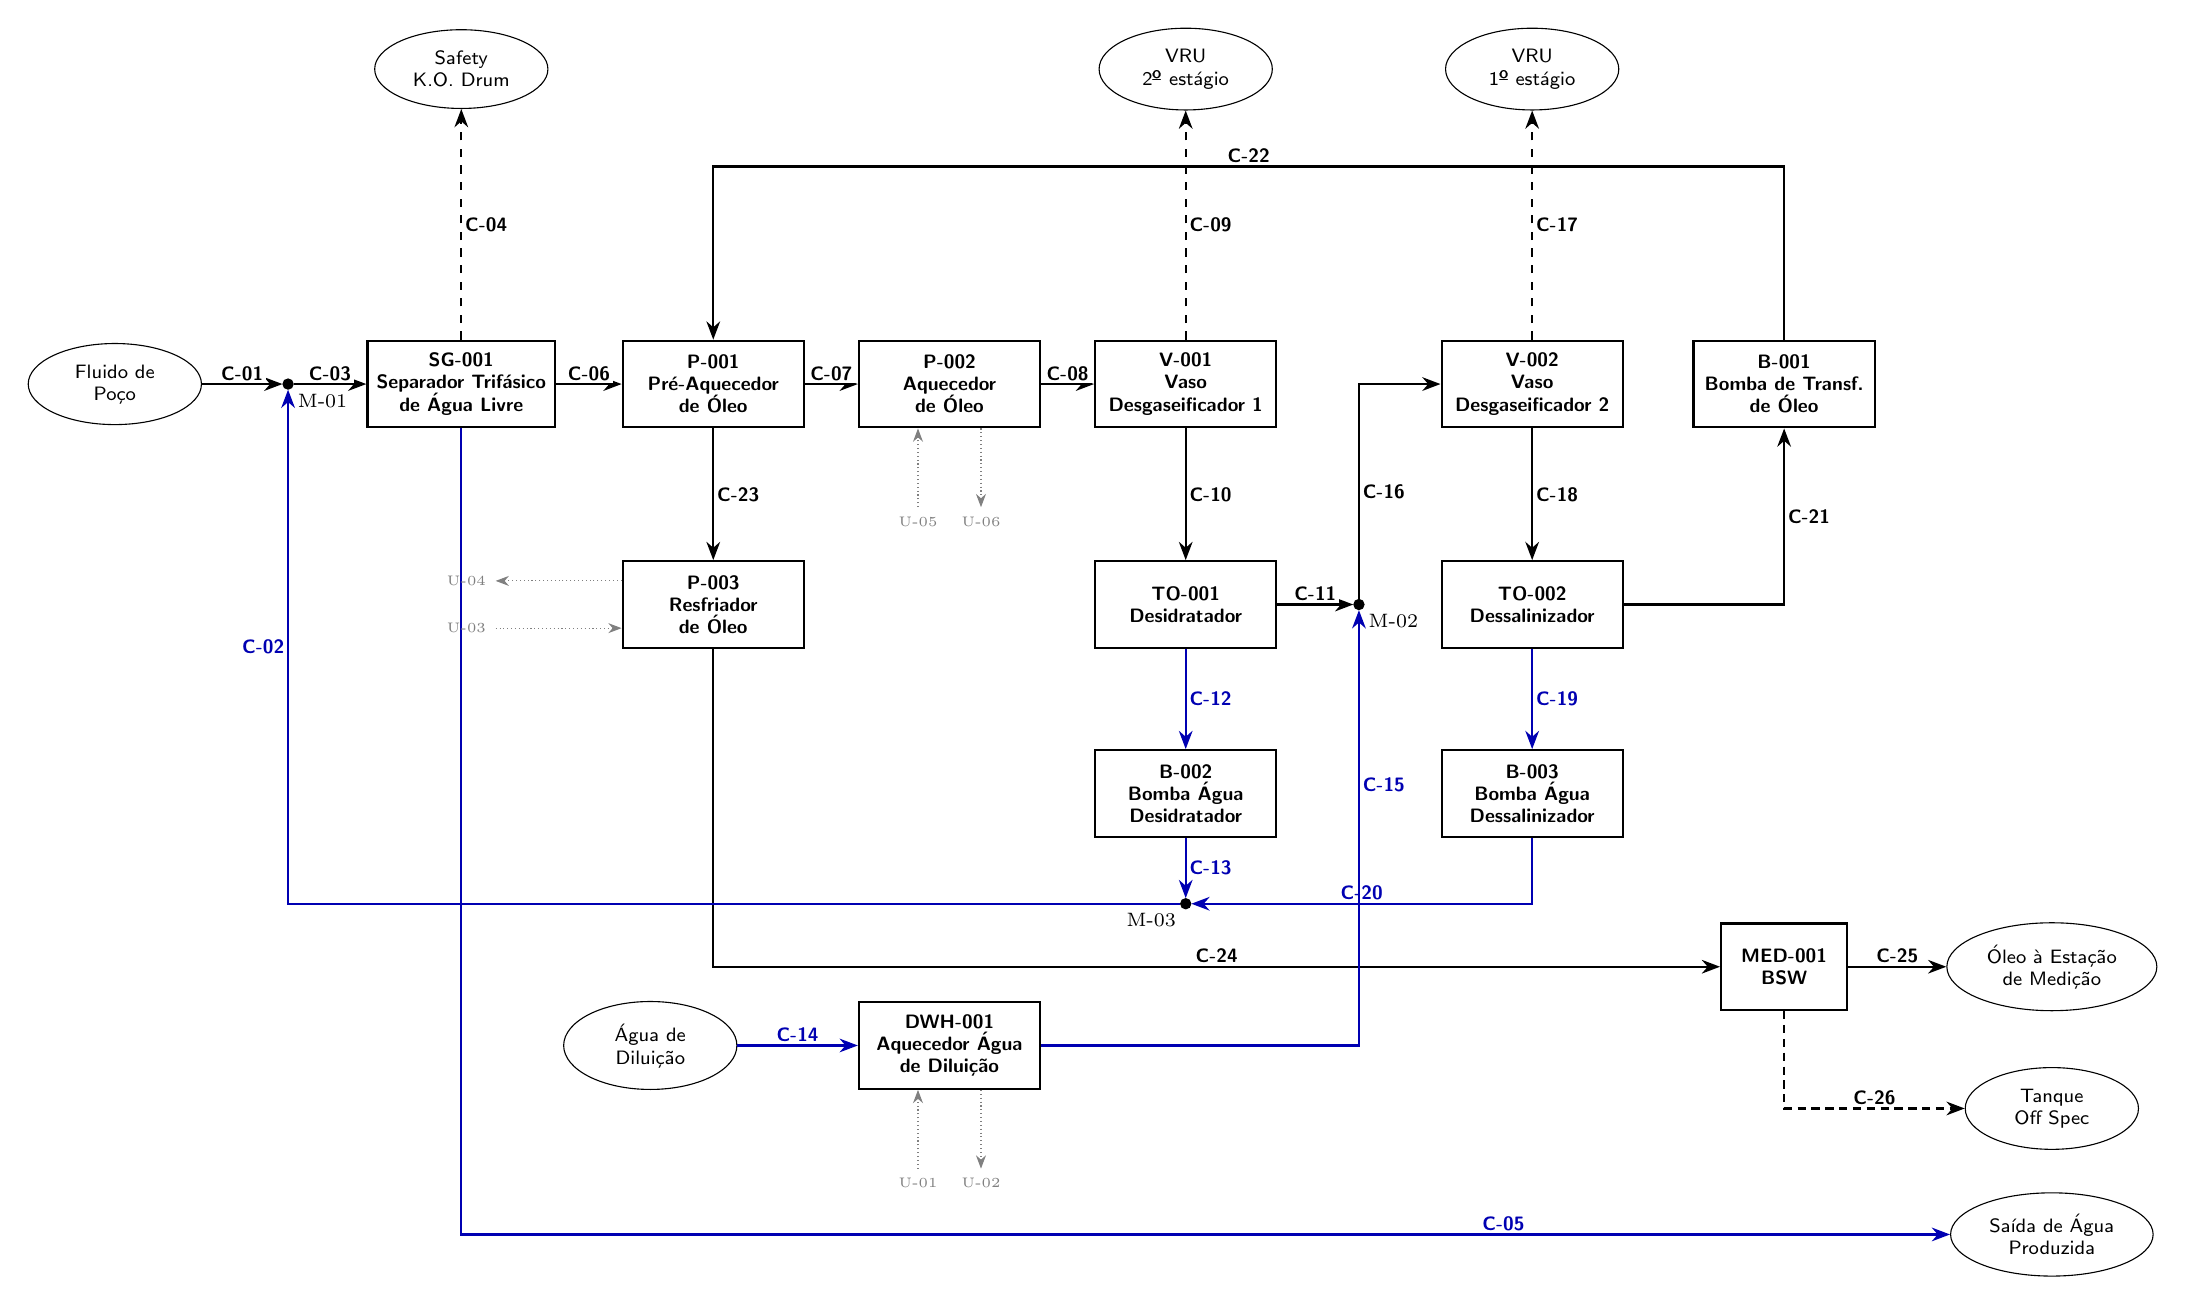
\begin{tikzpicture}[>=Stealth, font=\sffamily\small,
 blk/.style={draw,thick,minimum width=2.3cm,minimum height=1.1cm,align=center,fill=white,font=\sffamily\scriptsize\bfseries},
 ext/.style={draw,ellipse,minimum width=2.2cm,minimum height=1.0cm,align=center,font=\sffamily\scriptsize},
 nd/.style={circle,draw,fill=black,inner sep=1.3pt},
 lab/.style={font=\sffamily\scriptsize\bfseries,fill=white,inner sep=1pt},
 oil/.style={->,thick}, gas/.style={->,thick,dashed}, wat/.style={->,thick,blue!70!black}, utl/.style={->,thin,densely dotted,gray}]
\node[ext] (well) at (-1.2,4) {Fluido de\\Poço};
\node[nd] (m1) at (1.0,4) {}; \node[font=\scriptsize,below right] at (m1) {M-01};
\node[blk] (fwko) at (3.2,4) {SG-001\\Separador Trifásico\\de Água Livre};
\node[blk] (pa) at (6.4,4) {P-001\\Pré-Aquecedor\\de Óleo};
\node[blk] (aq) at (9.4,4) {P-002\\Aquecedor\\de Óleo};
\node[blk] (d1) at (12.4,4) {V-001\\Vaso\\Desgaseificador 1};
\node[blk] (des) at (12.4,1.2) {TO-001\\Desidratador};
\node[nd] (m2) at (14.6,1.2) {}; \node[font=\scriptsize,below right] at (m2) {M-02};
\node[blk] (d2) at (16.8,4) {V-002\\Vaso\\Desgaseificador 2};
\node[blk] (dsl) at (16.8,1.2) {TO-002\\Dessalinizador};
\node[blk] (bo) at (20.0,4) {B-001\\Bomba de Transf.\\de Óleo};
\node[blk] (res) at (6.4,1.2) {P-003\\Resfriador\\de Óleo};
\node[blk] (b1) at (12.4,-1.2) {B-002\\Bomba Água\\Desidratador};
\node[blk] (b2) at (16.8,-1.2) {B-003\\Bomba Água\\Dessalinizador};
\node[nd] (m3) at (12.4,-2.6) {}; \node[font=\scriptsize,below left] at (m3) {M-03};
\node[blk] (hd) at (9.4,-4.4) {DWH-001\\Aquecedor Água\\de Diluição};
\node[ext] (dil) at (5.6,-4.4) {Água de\\Diluição};
\node[blk,minimum width=1.6cm] (bsw) at (20.0,-3.4) {MED-001\\BSW};
\node[ext] (med) at (23.4,-3.4) {Óleo à Estação\\de Medição};
\node[ext] (off) at (23.4,-5.2) {Tanque\\Off Spec};
\node[ext] (agua) at (23.4,-6.8) {Saída de Água\\Produzida};
\node[ext] (ko) at (3.2,8.0) {Safety\\K.O. Drum};
\node[ext] (vru2) at (12.4,8.0) {VRU\\2º estágio};
\node[ext] (vru1) at (16.8,8.0) {VRU\\1º estágio};
\draw[oil] (well) -- node[lab,above]{C-01} (m1);
\draw[oil] (m1) -- node[lab,above]{C-03} (fwko);
\draw[gas] (fwko) -- node[lab,right]{C-04} (ko);
\draw[oil] (fwko) -- node[lab,above]{C-06} (pa);
\draw[oil] (pa) -- node[lab,above]{C-07} (aq);
\draw[oil] (aq) -- node[lab,above]{C-08} (d1);
\draw[gas] (d1) -- node[lab,right]{C-09} (vru2);
\draw[oil] (d1) -- node[lab,right]{C-10} (des);
\draw[oil] (des) -- node[lab,above]{C-11} (m2);
\draw[oil] (m2) |- node[lab,pos=0.25,right]{C-16} (d2);
\draw[gas] (d2) -- node[lab,right]{C-17} (vru1);
\draw[oil] (d2) -- node[lab,right]{C-18} (dsl);
\draw[oil] (dsl.east) -| node[lab,pos=0.75,right]{C-21} (bo.south);
\draw[oil] (bo.north) -- ++(0,2.2) -| node[lab,pos=0.25,above]{C-22} (pa.north);
\draw[oil] (pa.south) -- node[lab,right]{C-23} (res.north);
\draw[oil] (res.south) |- node[lab,pos=0.75,above]{C-24} (bsw.west);
\draw[oil] (bsw) -- node[lab,above]{C-25} (med);
\draw[oil,densely dashed] (bsw.south) |- node[lab,pos=0.75,above]{C-26} (off);
\draw[wat] (fwko.south) |- node[lab,above,pos=0.85]{C-05} (agua.west);
\draw[wat] (des) -- node[lab,right]{C-12} (b1);
\draw[wat] (dsl) -- node[lab,right]{C-19} (b2);
\draw[wat] (b1) -- node[lab,right]{C-13} (m3);
\draw[wat] (b2.south) |- node[lab,pos=0.75,above]{C-20} (m3);
\draw[wat] (m3) -- (1.0,-2.6) -- node[lab,left]{C-02} (m1);
\draw[wat] (dil) -- node[lab,above]{C-14} (hd);
\draw[wat] (hd.east) -| node[lab,pos=0.8,right]{C-15} (m2.south);
\draw[utl] (res.west) ++(-1.6,-0.3) node[left,font=\tiny]{U-03} -- ($(res.west)+(0,-0.3)$);
\draw[utl] ($(res.west)+(0,0.3)$) -- ++(-1.6,0) node[left,font=\tiny]{U-04};
\draw[utl] ($(hd.south)+(-0.4,-1.0)$) node[below,font=\tiny]{U-01} -- ($(hd.south)+(-0.4,0)$);
\draw[utl] ($(hd.south)+(0.4,0)$) -- ++(0,-1.0) node[below,font=\tiny]{U-02};
\draw[utl] ($(aq.south)+(-0.4,-1.0)$) node[below,font=\tiny]{U-05} -- ($(aq.south)+(-0.4,0)$);
\draw[utl] ($(aq.south)+(0.4,0)$) -- ++(0,-1.0) node[below,font=\tiny]{U-06};
\end{tikzpicture}}
\caption{Reprodução esquemática do DE-SEN-SEP-COO-001-0 com a codificação de correntes deste memorial. Linhas cheias: óleo; tracejadas: gás; azuis: água; pontilhadas: utilidades.}\label{fig:db}
\end{figure}
\end{landscape}

\section{Identificação e codificação das correntes}
As correntes de processo receberam o código C-NN, numeradas na ordem de primeira aparição ao percorrer o DB a partir da alimentação, e as utilidades receberam U-NN. Os equipamentos foram identificados pelos TAGs preliminares da Tabela~\ref{tab:tags}, empregados em todo o memorial e no fluxograma da Figura~\ref{fig:db}; os pontos de mistura e de junção, que não são equipamentos, receberam os códigos de nó M-01, M-02 e M-03. A numeração definitiva dos TAGs não foi estabelecida nesta etapa e foi mantida fora do escopo desta identificação preliminar: sua definição deverá ser realizada posteriormente, em conjunto com a lista de equipamentos e a documentação de engenharia correspondente.
\begin{longtable}{lL{5.6cm}L{2.8cm}L{1.9cm}L{2.5cm}}
\caption{Lista de correntes, origem e destino.}\label{tab:correntes}\\\toprule
Código & Descrição & Fase predominante & Origem & Destino\\\midrule\endfirsthead
\toprule Código & Descrição & Fase & Origem & Destino\\\midrule\endhead

C-01 & Fluido de poço (jusante do choke) — alimentação da unidade & Multifásica G/O/A & Poços & M-01\\
C-02 & Reciclo de água produzida (após válvula de reciclo) & Aquosa & M-03 & M-01\\
C-03 & Alimentação do FWKO (C-01 + C-02) & Multifásica G/O/A & M-01 & SG-001\\
C-04 & Gás do FWKO para o Safety K.O. Drum & Gás (névoa residual) & SG-001 & Limite de bateria\\
C-05 & Água produzida do FWKO (saída da unidade) & Aquosa (óleo disperso) & SG-001 & Limite de bateria\\
C-06 & Óleo/emulsão do FWKO ao pré-aquecedor (lado frio) & Emulsão + gás dissolvido & SG-001 & P-001\\
C-07 & Saída lado frio do pré-aquecedor & Emulsão + gás dissolvido & P-001 & P-002\\
C-08 & Saída do aquecedor de óleo ao desgaseificador 1 & Emulsão + gás dissolvido & P-002 & V-001\\
C-09 & Gás do desgaseificador 1 ao 2º estágio da VRU & Gás & V-001 & Limite de bateria\\
C-10 & Líquido do desgaseificador 1 ao desidratador & Emulsão + gás dissolvido & V-001 & TO-001\\
C-11 & Óleo do desidratador & Óleo úmido + gás dissolvido & TO-001 & M-02\\
C-12 & Água do desidratador à bomba & Aquosa & TO-001 & B-002\\
C-13 & Descarga da bomba de água do desidratador & Aquosa & B-002 & M-03\\
C-14 & Água de diluição (osmose inversa) ao aquecedor & Água doce & OI & DWH-001\\
C-15 & Água de diluição aquecida ao ponto de injeção & Água doce & DWH-001 & M-02\\
C-16 & Óleo + água de diluição ao desgaseificador 2 & Óleo úmido + gás dissolvido & M-02 & V-002\\
C-17 & Gás do desgaseificador 2 ao 1º estágio da VRU & Gás & V-002 & Limite de bateria\\
C-18 & Líquido do desgaseificador 2 ao dessalinizador & Óleo úmido & V-002 & TO-002\\
C-19 & Água do dessalinizador à bomba & Aquosa & TO-002 & B-003\\
C-20 & Descarga da bomba de água do dessalinizador & Aquosa & B-003 & M-03\\
C-21 & Óleo tratado à bomba de transferência & Óleo tratado & TO-002 & B-001\\
C-22 & Óleo tratado ao pré-aquecedor (lado quente) & Óleo tratado & B-001 & P-001\\
C-23 & Saída lado quente do pré-aquecedor ao resfriador & Óleo tratado & P-001 & P-003\\
C-24 & Óleo resfriado ao medidor de BSW & Óleo tratado & P-003 & MED-001\\
C-25 & Óleo à estação de medição (saída da unidade) & Óleo tratado & MED-001 & Limite de bateria\\
C-26 & Óleo off-spec ao tanque off-spec (saída eventual) & Óleo fora de especificação & MED-001 & Limite de bateria\\
\midrule
U-01/U-02 & Água quente / água fria do circuito de aquecimento (DWH-001) & Utilidade & -- & --\\
U-03/U-04 & Água fria / água quente do circuito de resfriamento (P-003) & Utilidade & -- & --\\
U-05/U-06 & Água quente / água fria do circuito de aquecimento (P-002) & Utilidade & -- & --\\
\bottomrule\end{longtable}
Na Tabela~\ref{tab:blocos} resume-se a topologia usada no balanço.
\begin{longtable}{lL{7cm}L{3cm}L{3.2cm}}
\caption{Equipamentos, nós e correntes de entrada/saída.}\label{tab:blocos}\\\toprule
TAG / nó & Nome & Entradas & Saídas\\\midrule\endfirsthead
\toprule TAG / nó & Nome & Entradas & Saídas\\\midrule\endhead

M-01 & Ponto de mistura de entrada (M-01) & C-01, C-02 & C-03\\
SG-001 & Separador trifásico de água livre (FWKO) & C-03 & C-04, C-05, C-06\\
P-001 & Pré-aquecedor óleo/óleo & C-06, C-22 & C-07, C-23\\
P-002 & Aquecedor de óleo & C-07, $\dot Q_{\mbox{P-002}}$ & C-08\\
V-001 & Vaso desgaseificador 1 (gás ao 2º estágio da VRU) & C-08 & C-09, C-10\\
TO-001 & Desidratador (pré-tratador eletrostático) & C-10 & C-11, C-12\\
B-002 & Bomba de água produzida do desidratador & C-12, $\dot W_{\mbox{B-002}}$ & C-13\\
DWH-001 & Aquecedor de água de diluição & C-14, $\dot Q_{\mbox{DWH-001}}$ & C-15\\
M-02 & Ponto de injeção de água de diluição (M-02) & C-11, C-15 & C-16\\
V-002 & Vaso desgaseificador 2 (gás ao 1º estágio da VRU) & C-16 & C-17, C-18\\
TO-002 & Dessalinizador (tratador eletrostático) & C-18 & C-19, C-21\\
B-003 & Bomba de água produzida do dessalinizador & C-19, $\dot W_{\mbox{B-003}}$ & C-20\\
M-03 & Nó de reciclo de água produzida (M-03) & C-13, C-20 & C-02\\
B-001 & Bomba de transferência de óleo & C-21, $\dot W_{\mbox{B-001}}$ & C-22\\
P-003 & Resfriador de óleo & C-23 & C-24, $\dot Q_{\mbox{P-003}}$\\
MED-001 & Medidor de BSW e desvio off-spec (Nota 1 do DB) & C-24 & C-25, C-26\\
\bottomrule\end{longtable}
\subsection{Identificação preliminar de equipamentos}
Nem o DB (DE-SEN-SEP-COO-001-0) nem a ET (I-ET-3010.2K-1200-941-P4X-001\_C) atribuem TAG aos equipamentos ou aos pontos de mistura do módulo: o DB identifica os blocos pela função e a ET, pelo item de texto. Os TAGs da Tabela~\ref{tab:tags} são, portanto, designações preliminares adotadas neste memorial e no fluxograma da Figura~\ref{fig:db} apenas para permitir a referência unívoca a cada equipamento; não reproduzem a nomenclatura de numeração da operadora e não constituem TAG de projeto.
\small\begin{longtable}{rllL{6.8cm}}
\caption{TAGs preliminares adotados neste memorial.}\label{tab:tags}\\\toprule
Ordem & TAG preliminar & Tipo & Equipamento\\\midrule\endfirsthead
\toprule Ordem & TAG preliminar & Tipo & Equipamento\\\midrule\endhead
1 & SG-001 & Separador & Separador trifásico de água livre --- FWKO\\
2 & P-001 & Permutador & Pré-aquecedor de óleo (óleo/óleo)\\
3 & P-002 & Permutador & Aquecedor de óleo\\
4 & V-001 & Vaso & Desgaseificador --- 1º estágio\\
5 & TO-001 & Tratador & Desidratador eletrostático --- 1º estágio\\
6 & B-002 & Bomba & Bomba de água produzida --- desidratador\\
7 & DWH-001 & Permutador & Aquecedor de água de diluição\\
8 & V-002 & Vaso & Desgaseificador --- 2º estágio\\
9 & TO-002 & Tratador & Desidratador eletrostático --- 2º estágio (dessalinizador)\\
10 & B-003 & Bomba & Bomba de água produzida --- dessalinizador\\
11 & B-001 & Bomba & Bomba de transferência de óleo\\
12 & P-003 & Permutador & Resfriador de óleo\\
\midrule
-- & M-01 & Nó & Ponto de mistura do reciclo de água com o fluido de poço\\
-- & M-02 & Nó & Ponto de injeção da água de diluição\\
-- & M-03 & Nó & Junção das descargas das bombas de água produzida\\
-- & MED-001 & Instrumento & Medidor de BSW e desvio off-spec (designação provisória: sem identificação própria no DB nem na ET)\\
\bottomrule\end{longtable}\normalsize
\subsection{Parâmetros de operação estabelecidos e não estabelecidos pela ET}\label{sec:etparams}
A ET fixa os seguintes parâmetros do trecho de tratamento de óleo, adotados neste memorial como dado de fonte: temperatura de tratamento na entrada dos tratadores eletrostáticos de no mínimo 90~\si{\celsius} (item 2.7.1.4), temperatura máxima do meio de aquecimento de 120~\si{\celsius} (item 2.7.1.4), temperatura de armazenamento de 40~\si{\celsius} e temperatura de separação máxima de 99~\si{\celsius} (item 2.7.1.10), manutenção da entrada do FWKO em 40~\si{\celsius} por recirculação de água ou de óleo (item 2.7.1.6), pressão do FWKO (arquivo de casos) e as especificações do óleo tratado (item 2.3.1.1).

A ET \textbf{não} estabelece, para este trecho: as pressões de operação dos desgaseificadores e dos tratadores eletrostáticos; a pressão de descarga da bomba de transferência de óleo; as vazões (ou frações) de recirculação de água produzida e de óleo; a vazão, a temperatura e a salinidade da água de diluição; as quedas de pressão dos trocadores; e as temperaturas dos circuitos de água de aquecimento e de resfriamento. Nenhum desses valores foi extraído de outra fonte nem assumido como dado de projeto: onde o fechamento do modelo exigiu um valor, ele foi declarado como premissa numerada na Tabela~\ref{tab:premissas} (P-17 a P-22, P-30, P-31, P-36) e mantido nessa classificação. Recomenda-se que esses parâmetros sejam obtidos do Fluxograma de Processo (PFD) do módulo quando este estiver disponível, conforme os itens 3, 6, 7, 10, 13 e 14 da Tabela~\ref{tab:info}.

Registra-se ainda uma diferença entre as duas fontes quanto ao ponto de injeção da água de diluição: a ET, no item 2.7.1.6, indica a injeção a montante do aquecedor de óleo (e, no item 2.7.1.7, a adição de água de diluição no estágio final de tratamento), enquanto o DB (Nota~2) a posiciona entre o desidratador e o desgaseificador do 2º estágio. Este memorial seguiu o DB, por ser o documento que define a sequência aqui quantificada; a definição do ponto de injeção foi recomendada para verificação no PFD (item 29 da Tabela~\ref{tab:info}).

\section{Balanço preliminar do processo global}\label{sec:global}
Volume de controle: todos os equipamentos e nós, de M-01 a MED-001. Entradas: C-01, C-14, $\dot Q_{\mbox{P-002}}$, $\dot Q_{\mbox{DWH-001}}$ e $\sum\dot W$; saídas: C-04, C-05, C-09, C-17, C-25, C-26 e $\dot Q_{\mbox{P-003}}$. As correntes do laço (C-02, C-13, C-20) são internas. Em regime permanente:
\begin{equation}\label{eq:mglobal}
\sum_{\mathrm{in}}\dot m=\sum_{\mathrm{out}}\dot m,\qquad \varepsilon_m=\frac{\left|\sum\dot m_{\mathrm{in}}-\sum\dot m_{\mathrm{out}}\right|}{\sum\dot m_{\mathrm{in}}},
\end{equation}
\begin{equation}\label{eq:eglobal}
\dot Q-\dot W+\sum_{\mathrm{in}}\dot m\left(h+\tfrac{v^2}{2}+gz\right)=\sum_{\mathrm{out}}\dot m\left(h+\tfrac{v^2}{2}+gz\right),
\end{equation}
que, com P-14, reduz-se a
\begin{equation}\label{eq:eglobal2}
\sum_{\mathrm{in}}\dot H+\dot Q_{\mbox{P-002}}+\dot Q_{\mbox{DWH-001}}+\sum|\dot W|=\sum_{\mathrm{out}}\dot H+\dot Q_{\mbox{P-003}},
\end{equation}
\begin{equation}\label{eq:hsens}
\dot H=\sum_{k\in\{O,A,D,G\}}\dot m_k\,c_{p,k}\,(T-T_{\mathrm{ref}}),\qquad \varepsilon_E=\frac{\left|E_{\mathrm{in}}-E_{\mathrm{out}}\right|}{E_{\mathrm{in}}}.
\end{equation}
O sinal de $\dot W$ segue a convenção de trabalho realizado pelo sistema; como as bombas recebem trabalho, $-\dot W=|\dot W|$ entra do lado das entradas. O laço de reciclo foi resolvido por substituição sucessiva até variação $<10^{-10}$ nas vazões e temperaturas; os erros residuais refletem essa tolerância e o arredondamento em ponto flutuante, \textbf{não} a validade física do modelo (que depende das premissas).
\begin{landscape}
\small
\begin{longtable}{rrrrrrrrrrrr}
\caption{Balanço global por caso. Vazões em \si{\kilogram\per\second}; energias em \si{\mega\watt} (referência 15,6~\si{\celsius}).}\label{tab:global}\\\toprule
Caso & $\dot m_{C01}$ & $\dot m_{C14}$ & $\dot m_{C04+C09+C17}$ & $\dot m_{C05}$ & $\dot m_{C25}$ & $\varepsilon_m$ & $E_{\mathrm{in}}$ & $E_{\mathrm{out}}$ & $\dot Q_{\mathrm{aq}}$ & $\dot Q_{\mathrm{resf}}$ & $\varepsilon_E$\\\midrule\endfirsthead
\toprule Caso & $\dot m_{C01}$ & $\dot m_{C14}$ & gás & $\dot m_{C05}$ & $\dot m_{C25}$ & $\varepsilon_m$ & $E_{\mathrm{in}}$ & $E_{\mathrm{out}}$ & $\dot Q_{\mathrm{aq}}$ & $\dot Q_{\mathrm{resf}}$ & $\varepsilon_E$\\\midrule\endhead

1 & 451,92 & 0,00 & 157,42 & 0,00 & 294,51 & $1{,}3\times10^{-16}$ & 47,25 & 47,25 & 5,76 & 20,62 & $0$\\
2 & 494,41 & 10,73 & 157,42 & 51,60 & 296,12 & $2{,}6\times10^{-14}$ & 47,87 & 47,87 & 13,44 & 15,74 & $4{,}1\times10^{-14}$\\
3 & 453,82 & 10,73 & 118,11 & 51,60 & 294,83 & $2{,}9\times10^{-14}$ & 45,80 & 45,80 & 13,36 & 15,87 & $4{,}4\times10^{-14}$\\
4 & 50,08 & 0,00 & 11,81 & 0,00 & 38,28 & $0$ & 3,60 & 3,60 & 0,77 & 1,15 & $1{,}3\times10^{-16}$\\
5 & 60,15 & 0,00 & 10,32 & 0,00 & 49,83 & $0$ & 3,38 & 3,38 & 1,01 & 0,50 & $1{,}3\times10^{-16}$\\
6 & 25,24 & 0,00 & 12,38 & 0,00 & 12,86 & $1{,}4\times10^{-16}$ & 1,12 & 1,12 & 0,26 & 0,13 & $0$\\
7 & 432,03 & 0,00 & 137,52 & 0,00 & 294,51 & $0$ & 52,82 & 52,82 & 5,70 & 26,51 & $2{,}8\times10^{-16}$\\
8 & 503,77 & 7,14 & 137,52 & 176,21 & 197,18 & $2{,}6\times10^{-14}$ & 69,36 & 69,36 & 16,90 & 16,03 & $2{,}8\times10^{-14}$\\
9 & 516,28 & 5,61 & 137,52 & 229,52 & 154,85 & $1{,}8\times10^{-14}$ & 75,52 & 75,52 & 12,57 & 13,07 & $2{,}0\times10^{-14}$\\
10 & 456,71 & 4,30 & 109,70 & 232,69 & 118,62 & $1{,}8\times10^{-14}$ & 87,21 & 87,21 & 1,17 & 12,09 & $1{,}4\times10^{-14}$\\
11 & 532,03 & 2,96 & 131,64 & 321,62 & 81,72 & $4{,}9\times10^{-15}$ & 65,17 & 65,17 & 9,38 & 4,99 & $5{,}8\times10^{-15}$\\
12 & 531,71 & 3,00 & 131,64 & 320,29 & 82,78 & $6{,}0\times10^{-15}$ & 105,66 & 105,66 & 0,81 & 8,42 & $5{,}4\times10^{-15}$\\
13 & 537,23 & 3,60 & 142,07 & 299,35 & 99,41 & $7{,}1\times10^{-15}$ & 103,34 & 103,34 & 0,98 & 10,12 & $5{,}6\times10^{-15}$\\
14 & 578,48 & 3,60 & 183,32 & 299,35 & 99,41 & $6{,}6\times10^{-15}$ & 107,23 & 107,23 & 0,98 & 10,12 & $5{,}2\times10^{-15}$\\
15 & 526,29 & 1,30 & 112,39 & 379,22 & 35,99 & $2{,}2\times10^{-15}$ & 109,43 & 109,43 & 0,35 & 3,66 & $2{,}9\times10^{-15}$\\
16 & 533,73 & 1,45 & 121,03 & 374,08 & 40,07 & $6{,}6\times10^{-15}$ & 109,50 & 109,50 & 0,39 & 4,07 & $9{,}8\times10^{-15}$\\
\bottomrule\end{longtable}
\end{landscape}

\begin{longtable}{rrrrrrr}
\caption{Balanço molar global dos componentes ácidos do gás (\si{\kilo\mole\per\hour}), com $\dot n_i=y_i\dot m_G/\bar M_G$.}\label{tab:molar}\\\toprule
Caso & CO$_2$ in (C-01) & CO$_2$ out (gás) & $\varepsilon$ & H$_2$S in & H$_2$S out & $\varepsilon$\\\midrule\endfirsthead
\toprule Caso & CO$_2$ in & CO$_2$ out & $\varepsilon$ & H$_2$S in & H$_2$S out & $\varepsilon$\\\midrule\endhead

1 & 4.884,3 & 4.884,3 & $1{,}9\times10^{-16}$ & 3,336 & 3,336 & $1{,}3\times10^{-16}$\\
2 & 4.884,3 & 4.884,3 & $0$ & 3,336 & 3,336 & $0$\\
3 & 3.279,8 & 3.279,8 & $1{,}4\times10^{-16}$ & 2,466 & 2,466 & $0$\\
4 & 366,3 & 366,3 & $0$ & 0,250 & 0,250 & $0$\\
5 & 51,4 & 51,4 & $0$ & 0,273 & 0,273 & $0$\\
6 & 485,0 & 485,0 & $0$ & 0,215 & 0,215 & $0$\\
7 & 5.389,2 & 5.389,2 & $0$ & 2,385 & 2,385 & $0$\\
8 & 5.389,2 & 5.389,2 & $0$ & 2,385 & 2,385 & $0$\\
9 & 5.389,2 & 5.389,2 & $0$ & 2,385 & 2,385 & $0$\\
10 & 5.220,3 & 5.220,3 & $0$ & 2,423 & 2,423 & $0$\\
11 & 6.264,3 & 6.264,3 & $2{,}9\times10^{-16}$ & 2,908 & 2,908 & $0$\\
12 & 6.264,3 & 6.264,3 & $0$ & 2,908 & 2,908 & $0$\\
13 & 7.439,0 & 7.439,0 & $1{,}2\times10^{-16}$ & 3,028 & 3,028 & $2{,}9\times10^{-16}$\\
14 & 9.598,7 & 9.598,7 & $0$ & 3,907 & 3,907 & $2{,}3\times10^{-16}$\\
15 & 6.902,8 & 6.902,8 & $1{,}3\times10^{-16}$ & 2,091 & 2,091 & $2{,}1\times10^{-16}$\\
16 & 7.433,8 & 7.433,8 & $2{,}4\times10^{-16}$ & 2,252 & 2,252 & $0$\\
\bottomrule\end{longtable}

\section{Balanço preliminar equipamento a equipamento}\label{sec:blocos}
Cada equipamento ou nó foi apresentado no formato padronizado. As substituições numéricas utilizaram o \textbf{Caso 8 como caso de demonstração}, escolhido por ativar todos os blocos simultaneamente (água produzida não nula, $T_{C01}<90$~\si{\celsius}, carga de aquecimento e água de diluição não nulas). Essa escolha foi didática e \textbf{não} constituiu seleção de caso de projeto. Os resultados de todos os casos constam das tabelas de cada bloco e do Apêndice~\ref{app:correntes}.

\subsection{M-01 --- Ponto de mistura de entrada (M-01)}
\paragraph{Função:} nó do DB onde o reciclo de água produzida dos tratadores (C-02) encontra o fluido de poço (C-01) antes do FWKO, com o objetivo operacional de manter a entrada do FWKO a 40~\si{\celsius} (Nota~3 do DB; BOT 2.7.1.6). Não é equipamento; é volume de controle de mistura.
\paragraph{Entradas:} C-01: óleo 19.081 m³/d, água 12.721 m³/d, gás 10.000.000 Sm³/d, $T=60,0$~\si{\celsius}, $P=2.500$~\si{\kilo\pascal} (Caso 8); C-02: água 13.243 m³/d, $T=90,71$~\si{\celsius}.
\paragraph{Premissas:} P-06, P-14, P-15, P-16, P-21 (válvula de reciclo 2.600$\to$2.500~\si{\kilo\pascal}, isentálpica), P-36.
\paragraph{Modelo de cálculo:} 
\begin{equation}
\dot m_{k,C03}=\dot m_{k,C01}+\dot m_{k,C02},\qquad T_{C03}=\frac{\dot C_{C01}T_{C01}+\dot C_{C02}T_{C02}}{\dot C_{C01}+\dot C_{C02}},\qquad \dot C=\sum_k\dot m_k c_{p,k}.
\end{equation}
\begin{equation}
T_{C03}=\frac{1.161{,}4\times60{,}0+597{,}0\times90{,}71}{1.161{,}4+597{,}0}=70{,}43\ \si{\celsius}.
\end{equation}
\paragraph{Saídas:} C-03 multifásica a 70,43~\si{\celsius} e 2.500~\si{\kilo\pascal}, $\dot m=679,04$~\si{\kilogram\per\second} (Caso 8).
\paragraph{Balanço de massa:} $\varepsilon_m=$$1{,}9\times10^{-14}$ (Caso 8); todos os casos na Tabela~\ref{tab:b01}.
\paragraph{Balanço de energia:} mistura adiabática, $\varepsilon_E=$$2{,}0\times10^{-14}$.
\paragraph{Resultado preliminar:} a meta de 40~\si{\celsius} na entrada do FWKO \textbf{não} é atendida nos casos 5, 6, que têm BSW nulo e portanto nenhuma água disponível para reciclo; o BOT (Nota~11) prevê reciclo de óleo nessa situação, arranjo não incluído no DB desta etapa (P-41); sua avaliação foi recomendada na revisão posterior do diagrama.
\paragraph{Validação recomendada em etapa posterior:} vazão de reciclo controlada (o modelo assume todo o volume dos tratadores recirculado); inclusão de reciclo de óleo no DB; pressão real do coletor de produção.
{\footnotesize\setlength{\tabcolsep}{3.5pt}\begin{longtable}{rrrrrrrrrr}
\caption{M-01 --- mistura de entrada (todos os casos).\label{tab:b01}}\\\toprule
Caso & $\dot m_{C01}$ & $T_{C01}$ & $Q_{A+D,C02}$ & $T_{C02}$ & $\dot m_{C03}$ & $T_{C03}$ & $T\ge40$? & $\varepsilon_m$ & $\varepsilon_E$\\
 & kg/s & °C & m³/d & °C & kg/s & °C &  & -- & --\\\midrule\endfirsthead
\toprule Caso & $\dot m_{C01}$ & $T_{C01}$ & $Q_{A+D,C02}$ & $T_{C02}$ & $\dot m_{C03}$ & $T_{C03}$ & $T\ge40$? & $\varepsilon_m$ & $\varepsilon_E$\\\midrule\endhead
1 & 451,92 & 65,0 & 0 & -- & 451,92 & 65,00 & sim & $0$ & $0$\\
2 & 494,41 & 50,0 & 3.965 & 90,73 & 544,84 & 56,42 & sim & $2{,}4\times10^{-14}$ & $4{,}2\times10^{-14}$\\
3 & 453,82 & 50,0 & 3.965 & 90,73 & 504,25 & 56,76 & sim & $2{,}6\times10^{-14}$ & $4{,}4\times10^{-14}$\\
4 & 50,08 & 45,0 & 0 & -- & 50,08 & 45,00 & sim & $0$ & $0$\\
5 & 60,15 & 35,0 & 0 & -- & 60,15 & 35,00 & \textbf{não} & $0$ & $0$\\
6 & 25,24 & 35,0 & 0 & -- & 25,24 & 35,00 & \textbf{não} & $0$ & $0$\\
7 & 432,03 & 75,0 & 0 & -- & 432,03 & 75,00 & sim & $0$ & $0$\\
8 & 503,77 & 60,0 & 13.243 & 90,71 & 679,04 & 70,43 & sim & $1{,}9\times10^{-14}$ & $2{,}0\times10^{-14}$\\
9 & 516,28 & 65,0 & 10.400 & 90,71 & 654,22 & 71,97 & sim & $1{,}5\times10^{-14}$ & $1{,}5\times10^{-14}$\\
10 & 456,71 & 90,0 & 7.967 & 90,93 & 562,45 & 90,22 & sim & $1{,}5\times10^{-14}$ & $1{,}1\times10^{-14}$\\
11 & 532,03 & 55,0 & 5.488 & 90,71 & 604,96 & 60,33 & sim & $4{,}3\times10^{-15}$ & $5{,}3\times10^{-15}$\\
12 & 531,71 & 90,0 & 5.560 & 90,84 & 605,59 & 90,13 & sim & $5{,}4\times10^{-15}$ & $4{,}7\times10^{-15}$\\
13 & 537,23 & 90,0 & 6.676 & 90,86 & 625,92 & 90,16 & sim & $6{,}0\times10^{-15}$ & $5{,}0\times10^{-15}$\\
14 & 578,48 & 90,0 & 6.676 & 90,86 & 667,17 & 90,15 & sim & $5{,}8\times10^{-15}$ & $4{,}5\times10^{-15}$\\
15 & 526,29 & 90,0 & 2.417 & 90,76 & 558,43 & 90,05 & sim & $1{,}8\times10^{-15}$ & $2{,}9\times10^{-15}$\\
16 & 533,73 & 90,0 & 2.691 & 90,77 & 569,51 & 90,06 & sim & $6{,}2\times10^{-15}$ & $9{,}4\times10^{-15}$\\
\bottomrule\end{longtable}}
\subsection{SG-001 --- Separador trifásico de água livre (FWKO)}
\paragraph{Função:} primeiro estágio de separação: separa o gás livre (ao Safety K.O. Drum), a água livre (à saída de água produzida) e o óleo/emulsão com gás dissolvido (ao pré-aquecedor). Possui dispositivo ciclônico ou de palhetas para névoa (BOT 2.7.1.3).
\paragraph{Entradas:} C-03 (Caso 8): óleo 19.111 m³/d, água 25.964 m³/d, gás 10.000.000 Sm³/d, $T=70,43$~\si{\celsius}, $P=2.500$~\si{\kilo\pascal}; composição do gás na Tabela~\ref{tab:fluidprops}.
\paragraph{Premissas:} F-02, F-06, F-12, P-23, P-24, P-25, P-26, P-27, P-34, P-15 (isotérmico).
\paragraph{Modelo de cálculo:} foram utilizadas três eficiências distintas.
\emph{(i) Separação gás/líquido.} A liberação de gás foi estimada pela razão de solubilidade de Standing (\tipo{CORRELAÇÃO}, P-23), com $P$ em psia, $T$ em °F, $R_s$ em scf/STB e $1$~scf/STB$=0{,}178108$~Sm³/Sm³:
\begin{equation}\label{eq:standing}
R_s=\gamma_g\left[\left(\frac{P}{18{,}2}+1{,}4\right)10^{\,0{,}0125\,\mathrm{API}-0{,}00091\,T}\right]^{1{,}2048},\qquad \Delta R_s(P,T)=R_s(P,T)-R_s(P_{\mathrm{std}},T_{\mathrm{std}}).
\end{equation}
\begin{align}
Q_{G,C17}&=\Delta R_s(P_{\mbox{V-001}},T_{\mbox{V-001}})\,Q_O,\label{eq:gasstages}\\
Q_{G,C09}&=\left[\Delta R_s(P_{\mbox{SG-001}},T_{\mbox{SG-001}})-\Delta R_s(P_{\mbox{V-001}},T_{\mbox{V-001}})\right]Q_O,\nonumber\\
Q_{G,C04}&=Q_{G,\mathrm{in}}-Q_{G,C09}-Q_{G,C17}.\nonumber
\end{align}
Caso 8 ($\gamma_g=0{,}972$, API $=27{,}5$): $\Delta R_s(2.500\,\mathrm{kPa};70{,}4\,^\circ\mathrm{C})=12{,}01-1{,}00=11{,}01$~Sm³/Sm³ e $\Delta R_s(700\,\mathrm{kPa};90{,}0\,^\circ\mathrm{C})=1{,}858$~Sm³/Sm³, logo
\begin{equation}
Q_{G,C04}=10.000.000-174.565-35.457=9.789.978\ \mathrm{Sm^3/d}.
\end{equation}
A eficiência de separação gás/líquido do FWKO, no sentido de gás liberado recuperado na fase gás, é $\eta_{G}=Q_{G,C04}/Q_{G,\mathrm{in}}=0{,}9790$; o restante não é ineficiência mecânica, e sim gás em solução nas condições do vaso. A eficiência de remoção de líquido do gás é definida pelo arraste (P-26):
\begin{equation}
Q_{L,\mathrm{arraste}}=c_{\mathrm{arr}}\,Q_{G,C04},\qquad c_{\mathrm{arr}}=\frac{0{,}1\times3{,}785\times10^{-3}}{28\,316{,}8}=1{,}3368\times10^{-8}\ \mathrm{m^3/Sm^3}.
\end{equation}
\emph{(ii) Separação óleo/água.} Com $\mathrm{BSW}_{C01}$ da alimentação sem reciclo (P-24):
\begin{equation}\label{eq:bswF}
\mathrm{BSW}_{C06}=\min\left(0{,}40;\ \frac{Q_{A,C01}}{Q_{A,C01}+Q_{O,C01}}\right),\qquad Q_{A+D,C06}=\frac{\mathrm{BSW}_{C06}}{1-\mathrm{BSW}_{C06}}\,Q_{O,C03}.
\end{equation}
Justificativa da forma mínima: com toda a água dos tratadores retornando ao FWKO (P-36), um BSW de saída fixo em 40~\% sempre seria sustentado pelo próprio laço, qualquer que fosse a água produzida, e o estado estacionário deixaria de ser único. A eficiência de remoção de água livre resulta
\begin{equation}
\eta_{A,\mbox{SG-001}}=\frac{Q_{A+D,C05}}{Q_{A+D,C03}}=\frac{13.243}{25.964}=0{,}5101.
\end{equation}
\emph{(iii) Óleo na água} (P-25): $\dot m_{O,C05}=C_{OiW}\,Q_{A+D,C05}=2{,}0\ \mathrm{kg/m^3}\times13.243/86\,400=0{,}3066$~\si{\kilogram\per\second}.

\paragraph{Saídas:} C-04 gás 9.789.978 Sm³/d (134,633~\si{\kilogram\per\second}); C-05 água 13.243 m³/d; C-06 óleo 19.081 m³/d com BSW 40,0~\% e 210.022 Sm³/d de gás dissolvido. Todas a 70,43~\si{\celsius} e 2.500~\si{\kilo\pascal}.
\paragraph{Balanço de massa:} $\dot m_{C03}=679,038$; $\sum\dot m_{out}=679,038$~\si{\kilogram\per\second}; $\varepsilon_m=$$0$.
\paragraph{Balanço de energia:} vaso isotérmico e adiabático (P-15), $\varepsilon_E=$$0$. O resfriamento por liberação adicional de gás não é capturado.
\paragraph{Resultado preliminar:} maior gás separado no FWKO: 11.892.988 Sm³/d (caso 14); maior carga aquosa na entrada (incluindo reciclo): 30.678 m³/d (caso 15).
\paragraph{Validação recomendada em etapa posterior:} flash PR/CPA a 2.500~\si{\kilo\pascal} para substituir Standing (fora da faixa de validade para gás rico em CO$_2$); BSW de saída e teor de óleo na água por dados de fornecedor/simulação CFD; arraste do eliminador de névoa.
{\footnotesize\setlength{\tabcolsep}{3.5pt}\begin{longtable}{rrrrrrrrrrr}
\caption{SG-001 --- FWKO (todos os casos).\label{tab:b02}}\\\toprule
Caso & $Q_{G,C04}$ & $\eta_G$ & $Q_{A+D,C03}$ & $Q_{A+D,C05}$ & $\eta_A$ & BSW$_{C06}$ & $Q_{O,C06}$ & $T$ & $\varepsilon_m$ & $\varepsilon_E$\\
 & Sm³/d & -- & m³/d & m³/d & -- & \% & m³/d & °C & -- & --\\\midrule\endfirsthead
\toprule Caso & $Q_{G,C04}$ & $\eta_G$ & $Q_{A+D,C03}$ & $Q_{A+D,C05}$ & $\eta_A$ & BSW$_{C06}$ & $Q_{O,C06}$ & $T$ & $\varepsilon_m$ & $\varepsilon_E$\\\midrule\endhead
1 & 11.691.313 & 0,9743 & 0 & 0 & -- & 0,0 & 28.621 & 65,00 & $0$ & $1{,}8\times10^{-16}$\\
2 & 11.677.959 & 0,9732 & 7.146 & 3.965 & 0,5549 & 10,0 & 28.621 & 56,42 & $0$ & $0$\\
3 & 8.981.082 & 0,9657 & 7.146 & 3.965 & 0,5549 & 10,0 & 28.621 & 56,76 & $1{,}1\times10^{-16}$ & $1{,}6\times10^{-16}$\\
4 & 855.723 & 0,9508 & 0 & 0 & -- & 0,0 & 3.720 & 45,00 & $0$ & $0$\\
5 & 845.524 & 0,9395 & 0 & 0 & -- & 0,0 & 4.864 & 35,00 & $1{,}2\times10^{-16}$ & $0$\\
6 & 883.620 & 0,9818 & 0 & 0 & -- & 0,0 & 1.250 & 35,00 & $0$ & $0$\\
7 & 9.692.043 & 0,9692 & 0 & 0 & -- & 0,0 & 28.621 & 75,00 & $1{,}3\times10^{-16}$ & $0$\\
8 & 9.789.978 & 0,9790 & 25.964 & 13.243 & 0,5101 & 40,0 & 19.081 & 70,43 & $0$ & $0$\\
9 & 9.836.153 & 0,9836 & 27.202 & 17.212 & 0,6328 & 40,0 & 14.985 & 71,97 & $1{,}7\times10^{-16}$ & $1{,}5\times10^{-16}$\\
10 & 7.378.004 & 0,9837 & 25.088 & 17.435 & 0,6950 & 40,0 & 11.479 & 90,22 & $0$ & $1{,}3\times10^{-16}$\\
11 & 8.902.162 & 0,9891 & 29.340 & 24.068 & 0,8203 & 40,0 & 7.908 & 60,33 & $1{,}9\times10^{-16}$ & $0$\\
12 & 8.914.541 & 0,9905 & 29.310 & 23.969 & 0,8178 & 40,0 & 8.010 & 90,13 & $1{,}9\times10^{-16}$ & $0$\\
13 & 9.192.991 & 0,9885 & 28.823 & 22.410 & 0,7775 & 40,0 & 9.619 & 90,16 & $1{,}8\times10^{-16}$ & $1{,}2\times10^{-16}$\\
14 & 11.892.988 & 0,9911 & 28.823 & 22.410 & 0,7775 & 40,0 & 9.619 & 90,15 & $0$ & $1{,}1\times10^{-16}$\\
15 & 6.455.559 & 0,9932 & 30.678 & 28.356 & 0,9243 & 40,0 & 3.483 & 90,05 & $2{,}0\times10^{-16}$ & $2{,}5\times10^{-16}$\\
16 & 6.950.628 & 0,9929 & 30.559 & 27.974 & 0,9154 & 40,0 & 3.877 & 90,06 & $0$ & $1{,}2\times10^{-16}$\\
\bottomrule\end{longtable}}
\subsection{P-001 --- Pré-aquecedor óleo/óleo (casco e tubo)}
\paragraph{Função:} recuperar calor do óleo tratado quente (C-22, lado quente) para pré-aquecer o óleo/emulsão do FWKO (C-06, lado frio). BOT 2.7.1.5/2.7.1.11: casco e tubo com feixe removível, reserva instalada.
\paragraph{Entradas:} lado frio C-06: 368,19~\si{\kilogram\per\second}, 70,43~\si{\celsius}, 2.500~\si{\kilo\pascal}; lado quente C-22: 197,18~\si{\kilogram\per\second}, 90,48~\si{\celsius}, 800~\si{\kilo\pascal} (Caso 8).
\paragraph{Premissas:} P-14, P-17, P-32 (contracorrente, $\Delta T_{app}=10$~\si{\celsius}), P-10 a P-13. O lado quente depende de TO-002 e B-001, resolvidos no mesmo laço iterativo.
\paragraph{Modelo de cálculo:}
\begin{equation}\label{eq:preheat}
\dot Q_{\mbox{P-001}}=\dot C_{\min}\,\max\!\left(0;\ T_{C22}-T_{C06}-\Delta T_{app}\right),\qquad T_{C07}=T_{C06}+\frac{\dot Q_{\mbox{P-001}}}{\dot C_{C06}},\qquad T_{C23}=T_{C22}-\frac{\dot Q_{\mbox{P-001}}}{\dot C_{C22}}.
\end{equation}
Caso 8: $\dot C_{C06}=967{,}9$, $\dot C_{C22}=396{,}6$~\si{\kilo\watt\per\kelvin}; $\dot Q_{\mbox{P-001}}=396{,}6\times(90{,}48-70{,}43-10)=3.987$~\si{\kilo\watt}; $T_{C07}=74{,}55$~\si{\celsius}; $T_{C23}=80{,}43$~\si{\celsius}. Com $\dot C_{C22}<\dot C_{C06}$, a aproximação ocorre na extremidade fria (saída quente/entrada fria).

\paragraph{Saídas:} C-07 a 74,55~\si{\celsius} e 2.400~\si{\kilo\pascal}; C-23 a 80,43~\si{\celsius} e 700~\si{\kilo\pascal}. Sem mudança de composição.
\paragraph{Balanço de massa:} cada lado conserva massa; $\varepsilon_m=$$0$.
\paragraph{Balanço de energia:} $\dot C_{C06}(T_{C07}-T_{C06})=\dot C_{C22}(T_{C22}-T_{C23})$; $\varepsilon_E=$$1{,}8\times10^{-16}$.
\paragraph{Resultado preliminar:} maior carga recuperada: 14,33~\si{\mega\watt} (caso 2). Nos casos 10, 12, 13, 14, 15, 16 a alimentação chega a $\approx$90~\si{\celsius} e não há força motriz: o pré-aquecedor fica sem função térmica.
\paragraph{Validação recomendada em etapa posterior:} $\Delta T_{app}$ e $\Delta P$ pelo dimensionamento Bell--Delaware; propriedades da emulsão (viscosidade, $c_p$) e fator de incrustação.
{\footnotesize\setlength{\tabcolsep}{3.5pt}\begin{longtable}{rrrrrrrrrr}
\caption{P-001 --- pré-aquecedor (todos os casos).\label{tab:b03}}\\\toprule
Caso & $T_{C06}$ & $T_{C07}$ & $T_{C22}$ & $T_{C23}$ & $\dot C_{frio}$ & $\dot C_{quente}$ & $\dot Q_{\mbox{P-001}}$ & $\varepsilon_m$ & $\varepsilon_E$\\
 & °C & °C & °C & °C & kW/K & kW/K & MW & -- & --\\\midrule\endfirsthead
\toprule Caso & $T_{C06}$ & $T_{C07}$ & $T_{C22}$ & $T_{C23}$ & $\dot C_{frio}$ & $\dot C_{quente}$ & $\dot Q_{\mbox{P-001}}$ & $\varepsilon_m$ & $\varepsilon_E$\\\midrule\endhead
1 & 65,00 & 80,32 & 90,48 & 75,00 & 595 & 589 & 9,12 & $0$ & $0$\\
2 & 56,42 & 75,78 & 90,48 & 66,42 & 740 & 596 & 14,33 & $0$ & $1{,}9\times10^{-16}$\\
3 & 56,76 & 75,83 & 90,48 & 66,76 & 738 & 593 & 14,07 & $0$ & $1{,}9\times10^{-16}$\\
4 & 45,00 & 80,07 & 90,48 & 55,00 & 77 & 77 & 2,72 & $0$ & $2{,}3\times10^{-16}$\\
5 & 35,00 & 79,95 & 90,48 & 45,00 & 101 & 100 & 4,53 & $0$ & $1{,}9\times10^{-16}$\\
6 & 35,00 & 79,91 & 90,48 & 45,00 & 26 & 26 & 1,17 & $0$ & $0$\\
7 & 75,00 & 80,43 & 90,48 & 85,00 & 595 & 589 & 3,23 & $0$ & $0$\\
8 & 70,43 & 74,55 & 90,48 & 80,43 & 968 & 397 & 3,99 & $0$ & $1{,}8\times10^{-16}$\\
9 & 71,97 & 75,46 & 90,48 & 81,97 & 760 & 311 & 2,65 & $0$ & $0$\\
10 & 90,22 & 90,22 & 90,68 & 90,68 & 582 & 239 & 0,00 & $0$ & $0$\\
11 & 60,33 & 68,60 & 90,48 & 70,33 & 401 & 164 & 3,31 & $0$ & $1{,}2\times10^{-16}$\\
12 & 90,13 & 90,13 & 90,60 & 90,60 & 406 & 167 & 0,00 & $0$ & $0$\\
13 & 90,16 & 90,16 & 90,62 & 90,62 & 487 & 200 & 0,00 & $0$ & $0$\\
14 & 90,15 & 90,15 & 90,62 & 90,62 & 487 & 200 & 0,00 & $0$ & $0$\\
15 & 90,05 & 90,05 & 90,53 & 90,53 & 176 & 72 & 0,00 & $0$ & $0$\\
16 & 90,06 & 90,06 & 90,53 & 90,53 & 196 & 81 & 0,00 & $0$ & $0$\\
\bottomrule\end{longtable}}
\subsection{P-002 --- Aquecedor de óleo}
\paragraph{Função:} elevar a emulsão à temperatura de tratamento exigida na entrada dos tratadores eletrostáticos (mínimo 90~\si{\celsius}, BOT 2.7.1.4), com meio de aquecimento limitado a 120~\si{\celsius}.
\paragraph{Entradas:} C-07: 368,19~\si{\kilogram\per\second}, 74,55~\si{\celsius}, 2.400~\si{\kilo\pascal} (Caso 8).
\paragraph{Premissas:} F-05, P-14, P-17, P-33. O circuito de água de aquecimento (U-05/U-06) consta do DB; suas temperaturas e vazão não foram informadas e foram recomendadas para o balanço de utilidades posterior.
\paragraph{Modelo de cálculo:}
\begin{equation}\label{eq:heater}
T_{C08}=\max(90;\ T_{C07}),\qquad \dot Q_{\mbox{P-002}}=\sum_k\dot m_k\,h_{k,C08}-\sum_k\dot m_k\,h_{k,C07}=\dot C_{C07}\,(T_{C08}-T_{C07}).
\end{equation}
Caso 8: $\dot Q_{\mbox{P-002}}=967{,}9\times(90{,}00-74{,}55)=14.959$~\si{\kilo\watt}. A parcela de gás dissolvido é aquecida com $c_{p,G}$, sem calor de dessorção (P-14): a carga real tende a ser maior, pois parte do gás vaporiza a jusante.

\paragraph{Saídas:} C-08 a 90,00~\si{\celsius}, 2.300~\si{\kilo\pascal}.
\paragraph{Balanço de massa:} $\varepsilon_m=$$0$.
\paragraph{Balanço de energia:} $\varepsilon_E=$$2{,}0\times10^{-16}$.
\paragraph{Resultado preliminar:} maior carga: 14,96~\si{\mega\watt} (caso 8). Nenhum caso excede 99~\si{\celsius} (limite BOT 2.7.1.10): OK. Nos casos com chegada a 90~\si{\celsius} a temperatura de tratamento fica levemente acima de 90~\si{\celsius} pelo calor das bombas do laço.
\paragraph{Validação recomendada em etapa posterior:} vazão e temperaturas do circuito de aquecimento (balanço de utilidades); efeito do calor latente (flash) sobre a carga; margem de projeto do trocador.
{\footnotesize\setlength{\tabcolsep}{3.5pt}\begin{longtable}{rrrrrrrr}
\caption{P-002 --- aquecedor de óleo (todos os casos).\label{tab:b04}}\\\toprule
Caso & $\dot m_{C07}$ & $T_{C07}$ & $T_{C08}$ & $P_{C08}$ & $\dot Q_{\mbox{P-002}}$ & $\varepsilon_m$ & $\varepsilon_E$\\
 & kg/s & °C & °C & kPa & MW & -- & --\\\midrule\endfirsthead
\toprule Caso & $\dot m_{C07}$ & $T_{C07}$ & $T_{C08}$ & $P_{C08}$ & $\dot Q_{\mbox{P-002}}$ & $\varepsilon_m$ & $\varepsilon_E$\\\midrule\endhead
1 & 298,55 & 80,32 & 90,00 & 2.300 & 5,76 & $0$ & $0$\\
2 & 340,05 & 75,78 & 90,00 & 2.300 & 10,53 & $0$ & $1{,}3\times10^{-16}$\\
3 & 338,58 & 75,83 & 90,00 & 2.300 & 10,45 & $0$ & $2{,}7\times10^{-16}$\\
4 & 38,86 & 80,07 & 90,00 & 2.300 & 0,77 & $0$ & $0$\\
5 & 50,46 & 79,95 & 90,00 & 2.300 & 1,01 & $0$ & $0$\\
6 & 13,09 & 79,91 & 90,00 & 2.300 & 0,26 & $0$ & $0$\\
7 & 298,74 & 80,43 & 90,00 & 2.300 & 5,70 & $0$ & $0$\\
8 & 368,19 & 74,55 & 90,00 & 2.300 & 14,96 & $0$ & $2{,}0\times10^{-16}$\\
9 & 289,42 & 75,46 & 90,00 & 2.300 & 11,05 & $0$ & $1{,}3\times10^{-16}$\\
10 & 221,85 & 90,22 & 90,22 & 2.300 & 0,00 & $0$ & $0$\\
11 & 153,13 & 68,60 & 90,00 & 2.300 & 8,58 & $0$ & $1{,}2\times10^{-16}$\\
12 & 154,91 & 90,13 & 90,13 & 2.300 & 0,00 & $0$ & $0$\\
13 & 186,13 & 90,16 & 90,16 & 2.300 & 0,00 & $0$ & $0$\\
14 & 186,13 & 90,15 & 90,15 & 2.300 & 0,00 & $0$ & $0$\\
15 & 67,60 & 90,05 & 90,05 & 2.300 & 0,00 & $0$ & $0$\\
16 & 75,25 & 90,06 & 90,06 & 2.300 & 0,00 & $0$ & $0$\\
\bottomrule\end{longtable}}
\subsection{V-001 --- Vaso desgaseificador 1}
\paragraph{Função:} liberar o gás que sai de solução após o aquecimento e a redução de pressão de 2.300 para 700~\si{\kilo\pascal}, enviando-o ao 2º estágio da VRU. Forma conjunto com o pré-tratador (BOT 2.7.1.7: ``degasser/electrostatic pre-treater'').
\paragraph{Entradas:} C-08: 368,19~\si{\kilogram\per\second}, gás dissolvido 210.022 Sm³/d, 90,00~\si{\celsius}, 2.300~\si{\kilo\pascal} (Caso 8).
\paragraph{Premissas:} P-18, P-23, P-26, P-27, P-15 (válvula de nível isentálpica $\Rightarrow$ isotérmica no modelo sensível).
\paragraph{Modelo de cálculo:} válvula de entrada com $h_{\mathrm{in}}\approx h_{\mathrm{out}}$ e gás de \eqref{eq:gasstages}:
\begin{equation}
Q_{G,C09}=\left[11{,}007-1{,}858\right]\times19.081=174.565\ \mathrm{Sm^3/d},\qquad \eta_{G,\mbox{V-001}}=\frac{Q_{G,C09}}{Q_{G,\mathrm{dissolvido},C08}}=0{,}8312.
\end{equation}
Vazão real de gás com $Z=1$ (P-39): $Q_{G,\mathrm{real}}=Q_{G,\mathrm{std}}\frac{P_{\mathrm{std}}}{P}\frac{T}{T_{\mathrm{std}}}$.

\paragraph{Saídas:} C-09 gás 174.565 Sm³/d; C-10 líquido 365,79~\si{\kilogram\per\second}; ambas a 90,00~\si{\celsius} e 700~\si{\kilo\pascal}.
\paragraph{Balanço de massa:} $\varepsilon_m=$$0$.
\paragraph{Balanço de energia:} $\varepsilon_E=$$0$ (sem resfriamento por flash, P-15).
\paragraph{Resultado preliminar:} maior gás ao 2º estágio da VRU: 271.308 Sm³/d (caso 2).
\paragraph{Validação recomendada em etapa posterior:} pressão de operação (variável de decisão da futura otimização multiobjetivo); liberação real de gás por flash; temperatura após flash.
{\footnotesize\setlength{\tabcolsep}{3.5pt}\begin{longtable}{rrrrrrrr}
\caption{V-001 --- desgaseificador 1 (todos os casos).\label{tab:b05}}\\\toprule
Caso & $Q_{G,C09}$ & $Q_{G,real}$ & $\eta_{G}$ & $\dot m_{C10}$ & $T$ & $\varepsilon_m$ & $\varepsilon_E$\\
 & Sm³/d & m³/h & -- & kg/s & °C & -- & --\\\midrule\endfirsthead
\toprule Caso & $Q_{G,C09}$ & $Q_{G,real}$ & $\eta_{G}$ & $\dot m_{C10}$ & $T$ & $\varepsilon_m$ & $\varepsilon_E$\\\midrule\endhead
1 & 257.955 & 1.956 & 0,8356 & 295,17 & 90,00 & $0$ & $1{,}6\times10^{-16}$\\
2 & 271.308 & 2.057 & 0,8425 & 336,49 & 90,00 & $0$ & $1{,}3\times10^{-16}$\\
3 & 268.594 & 2.037 & 0,8422 & 335,17 & 90,00 & $1{,}7\times10^{-16}$ & $1{,}3\times10^{-16}$\\
4 & 37.683 & 286 & 0,8511 & 38,36 & 90,00 & $0$ & $0$\\
5 & 46.751 & 355 & 0,8582 & 49,92 & 90,00 & $0$ & $1{,}2\times10^{-16}$\\
6 & 14.058 & 107 & 0,8582 & 12,89 & 90,00 & $0$ & $1{,}2\times10^{-16}$\\
7 & 254.772 & 1.932 & 0,8273 & 295,24 & 90,00 & $1{,}9\times10^{-16}$ & $0$\\
8 & 174.565 & 1.324 & 0,8312 & 365,79 & 90,00 & $0$ & $0$\\
9 & 135.973 & 1.031 & 0,8299 & 287,55 & 90,00 & $2{,}0\times10^{-16}$ & $0$\\
10 & 99.301 & 754 & 0,8140 & 220,40 & 90,22 & $1{,}3\times10^{-16}$ & $0$\\
11 & 82.125 & 623 & 0,8394 & 151,93 & 90,00 & $0$ & $0$\\
12 & 69.558 & 528 & 0,8139 & 153,90 & 90,13 & $1{,}8\times10^{-16}$ & $0$\\
13 & 87.100 & 661 & 0,8140 & 184,80 & 90,16 & $0$ & $0$\\
14 & 87.102 & 661 & 0,8139 & 184,80 & 90,15 & $0$ & $0$\\
15 & 36.171 & 274 & 0,8139 & 66,97 & 90,05 & $2{,}1\times10^{-16}$ & $0$\\
16 & 40.184 & 305 & 0,8139 & 74,56 & 90,06 & $0$ & $1{,}2\times10^{-16}$\\
\bottomrule\end{longtable}}
\subsection{TO-001 --- Desidratador (pré-tratador eletrostático)}
\paragraph{Função:} coalescência eletrostática e decantação da água emulsionada, reduzindo o BSW para especificar o óleo ao estágio final (BOT 2.7.1.7).
\paragraph{Entradas:} C-10: óleo 19.081 m³/d, água 12.721 m³/d (BSW 40,0~\%), 90,00~\si{\celsius}, 700~\si{\kilo\pascal} (Caso 8).
\paragraph{Premissas:} P-18, P-25, P-28, P-34, P-15.
\paragraph{Modelo de cálculo:}
\begin{equation}
Q_{A+D,C11}=\min\!\left(\frac{\mathrm{BSW}_{\mbox{TO-001}}}{1-\mathrm{BSW}_{\mbox{TO-001}}}Q_{O,C10};\ Q_{A+D,C10}\right),\qquad \eta_{A,\mbox{TO-001}}=\frac{Q_{A+D,C12}}{Q_{A+D,C10}}.
\end{equation}
Caso 8: $Q_{A+D,C11}=\frac{0{,}01}{0{,}99}\times19.081=192{,}5$~m³/d; $\eta_{A,\mbox{TO-001}}=12.528/12.721=0{,}9849$.

\paragraph{Saídas:} C-11 óleo úmido com 192,5 m³/d de água; C-12 água 12.528 m³/d com óleo disperso (2.000 mg/L); ambas a 90,00~\si{\celsius}, 700~\si{\kilo\pascal}.
\paragraph{Balanço de massa:} $\varepsilon_m=$$1{,}6\times10^{-16}$.
\paragraph{Balanço de energia:} $\varepsilon_E=$$0$.
\paragraph{Resultado preliminar:} maior água removida: 12.528 m³/d (caso 8). Casos sem água produzida não têm água a remover.
\paragraph{Validação recomendada em etapa posterior:} BSW garantido pelo fornecedor em função da carga de água, temperatura, tempo de residência e campo elétrico; teor de óleo na água.
{\footnotesize\setlength{\tabcolsep}{3.5pt}\begin{longtable}{rrrrrrrr}
\caption{TO-001 --- desidratador (todos os casos).\label{tab:b06}}\\\toprule
Caso & $Q_{O,C10}$ & $Q_{A+D,C10}$ & $Q_{A+D,C11}$ & $Q_{A+D,C12}$ & $\eta_A$ & $\varepsilon_m$ & $\varepsilon_E$\\
 & m³/d & m³/d & m³/d & m³/d & -- & -- & --\\\midrule\endfirsthead
\toprule Caso & $Q_{O,C10}$ & $Q_{A+D,C10}$ & $Q_{A+D,C11}$ & $Q_{A+D,C12}$ & $\eta_A$ & $\varepsilon_m$ & $\varepsilon_E$\\\midrule\endhead
1 & 28.621 & 0 & 0,0 & 0 & -- & $0$ & $0$\\
2 & 28.621 & 3.181 & 289,0 & 2.892 & 0,9091 & $1{,}7\times10^{-16}$ & $0$\\
3 & 28.621 & 3.181 & 289,0 & 2.892 & 0,9091 & $0$ & $0$\\
4 & 3.720 & 0 & 0,0 & 0 & -- & $0$ & $0$\\
5 & 4.864 & 0 & 0,0 & 0 & -- & $0$ & $0$\\
6 & 1.250 & 0 & 0,0 & 0 & -- & $0$ & $0$\\
7 & 28.621 & 0 & 0,0 & 0 & -- & $0$ & $0$\\
8 & 19.081 & 12.721 & 192,5 & 12.528 & 0,9849 & $1{,}6\times10^{-16}$ & $0$\\
9 & 14.985 & 9.990 & 151,1 & 9.839 & 0,9849 & $0$ & $0$\\
10 & 11.479 & 7.652 & 115,8 & 7.537 & 0,9849 & $0$ & $1{,}7\times10^{-16}$\\
11 & 7.908 & 5.272 & 79,8 & 5.192 & 0,9849 & $0$ & $1{,}2\times10^{-16}$\\
12 & 8.010 & 5.340 & 80,8 & 5.260 & 0,9849 & $1{,}8\times10^{-16}$ & $0$\\
13 & 9.619 & 6.413 & 97,0 & 6.316 & 0,9849 & $1{,}5\times10^{-16}$ & $0$\\
14 & 9.619 & 6.413 & 97,0 & 6.316 & 0,9849 & $0$ & $0$\\
15 & 3.483 & 2.322 & 35,1 & 2.287 & 0,9849 & $0$ & $1{,}4\times10^{-16}$\\
16 & 3.877 & 2.585 & 39,1 & 2.546 & 0,9849 & $0$ & $1{,}2\times10^{-16}$\\
\bottomrule\end{longtable}}
\subsection{B-002 --- Bomba de água produzida do desidratador}
\paragraph{Função:} retornar a água removida no desidratador à entrada do FWKO (Nota~3 do DB).
\paragraph{Entradas:} C-12: 523,2 m³/h (massa específica padrão), 90,00~\si{\celsius}, 700~\si{\kilo\pascal} (Caso 8).
\paragraph{Premissas:} P-20/P-21, P-22, P-37. Perda de carga de sucção e NPSH não avaliados.
\paragraph{Modelo de cálculo:}
\begin{equation}
\dot W=\frac{\dot V\,(P_{d}-P_{s})}{\eta},\qquad T_{out}=T_{in}+\frac{\dot W}{\dot C}.
\end{equation}
Caso 8: $\dot W=\frac{0{,}14533\times(2.600-700)}{0{,}70}=394{,}46$~\si{\kilo\watt}; $\Delta T=0{,}701$~\si{\kelvin}.

\paragraph{Saídas:} C-13: 90,70~\si{\celsius}, 2.600~\si{\kilo\pascal}, mesma vazão.
\paragraph{Balanço de massa:} $\varepsilon_m=$$0$.
\paragraph{Balanço de energia:} $\dot H_{out}=\dot H_{in}+\dot W$; $\varepsilon_E=$$0$.
\paragraph{Resultado preliminar:} maior potência hidráulica/eixo preliminar: 394,5~\si{\kilo\watt} (caso 8).
\paragraph{Validação recomendada em etapa posterior:} pressões de sucção/descarga a definir pela hidráulica do sistema; curva e eficiência de fornecedor; configuração N+1.
{\footnotesize\setlength{\tabcolsep}{3.5pt}\begin{longtable}{rrrrrrrr}
\caption{B-002 --- Bomba de água produzida do desidratador (todos os casos).\label{tab:b002}}\\\toprule
Caso & $\dot V$ & $T_{in}$ & $T_{out}$ & $\Delta P$ & $\dot W$ & $\varepsilon_m$ & $\varepsilon_E$\\
 & m³/h & °C & °C & kPa & kW & -- & --\\\midrule\endfirsthead
\toprule Caso & $\dot V$ & $T_{in}$ & $T_{out}$ & $\Delta P$ & $\dot W$ & $\varepsilon_m$ & $\varepsilon_E$\\\midrule\endhead
1 & 0,0 & 90,00 & 90,00 & 1.900 & 0,0 & $0$ & $0$\\
2 & 120,8 & 90,00 & 90,69 & 1.900 & 91,1 & $0$ & $0$\\
3 & 120,8 & 90,00 & 90,69 & 1.900 & 91,1 & $0$ & $0$\\
4 & 0,0 & 90,00 & 90,00 & 1.900 & 0,0 & $0$ & $0$\\
5 & 0,0 & 90,00 & 90,00 & 1.900 & 0,0 & $0$ & $0$\\
6 & 0,0 & 90,00 & 90,00 & 1.900 & 0,0 & $0$ & $0$\\
7 & 0,0 & 90,00 & 90,00 & 1.900 & 0,0 & $0$ & $0$\\
8 & 523,2 & 90,00 & 90,70 & 1.900 & 394,5 & $0$ & $0$\\
9 & 410,9 & 90,00 & 90,70 & 1.900 & 309,8 & $0$ & $2{,}2\times10^{-16}$\\
10 & 314,7 & 90,22 & 90,92 & 1.900 & 237,3 & $0$ & $1{,}4\times10^{-16}$\\
11 & 216,8 & 90,00 & 90,70 & 1.900 & 163,5 & $0$ & $0$\\
12 & 219,6 & 90,13 & 90,83 & 1.900 & 165,6 & $0$ & $0$\\
13 & 263,8 & 90,16 & 90,86 & 1.900 & 198,9 & $0$ & $1{,}7\times10^{-16}$\\
14 & 263,8 & 90,15 & 90,85 & 1.900 & 198,9 & $0$ & $0$\\
15 & 95,5 & 90,05 & 90,76 & 1.900 & 72,0 & $0$ & $0$\\
16 & 106,3 & 90,06 & 90,76 & 1.900 & 80,2 & $0$ & $0$\\
\bottomrule\end{longtable}}
\subsection{DWH-001 --- Aquecedor de água de diluição}
\paragraph{Função:} aquecer a água de diluição (permeado de osmose inversa, BOT 2.7.1.7; Nota~2 do DB) antes da injeção no óleo, com água quente do circuito de aquecimento (U-01/U-02).
\paragraph{Entradas:} C-14: 618 m³/d a 25~\si{\celsius} (Caso 8); vazão definida pelo critério de salinidade abaixo.
\paragraph{Premissas:} F-09, F-10, P-29, P-30, P-31, P-09, P-12.
\paragraph{Modelo de cálculo:} balanço de sal com diluição ideal ($\eta_{mix}=1$) e água de C-11 à salinidade máxima:
\begin{equation}\label{eq:dil}
S_{\mathrm{res}}\le\frac{S_{\mathrm{spec}}}{\mathrm{BSW}_{\mbox{TO-002}}}=\frac{285}{0{,}005}=57.000\ \mathrm{mg/L},\qquad Q_{D}=Q_{A+D,C11}\left(\frac{S_A}{S_{\mathrm{res}}}-1\right)\frac{1}{\eta_{mix}},
\end{equation}
\begin{equation}
Q_D=192{,}5\times\left(\frac{240.000}{57.000}-1\right)=617{,}9\ \mathrm{m^3/d},
\end{equation}
\begin{equation}
\dot Q_{\mbox{DWH-001}}=\dot m_D\,c_{p,D}(T_{C15}-T_{C14})=7{,}144\times4{,}18\times(90-25)=1.941\ \mathrm{kW}.
\end{equation}
A relação $Q_D/Q_O=3{,}24$~\% (Caso 8). O resultado é um mínimo teórico: com mistura imperfeita a vazão cresce rapidamente (sensibilidade na Tabela~\ref{tab:sens}).

\paragraph{Saídas:} C-15: 618 m³/d a 90~\si{\celsius} e $\ge$700~\si{\kilo\pascal} (pressão de injeção assumida; a bomba de água de diluição não integra o DB desta etapa e sua especificação foi recomendada para etapa posterior).
\paragraph{Balanço de massa:} $\varepsilon_m=$$0$.
\paragraph{Balanço de energia:} $\varepsilon_E=$$2{,}0\times10^{-16}$.
\paragraph{Resultado preliminar:} maior vazão de diluição: 928 m³/d (caso 3). Nos casos 1, 4, 5, 6, 7 (BSW nulo) o critério de salinidade resulta em diluição nula; o BOT 2.7.1.6 recomenda diluição em baixo BSW para desempenho do pré-tratador, sem quantificá-la.
\paragraph{Validação recomendada em etapa posterior:} vazão de projeto da osmose inversa; eficiência de mistura da válvula; salinidade do permeado; temperatura disponível do permeado; pressão de injeção.
{\footnotesize\setlength{\tabcolsep}{3.5pt}\begin{longtable}{rrrrrrr}
\caption{DWH-001 --- aquecedor de água de diluição (todos os casos).\label{tab:b08}}\\\toprule
Caso & $Q_{A+D,C11}$ & $Q_D$ & $Q_D/Q_O$ & $\dot Q_{\mbox{DWH-001}}$ & $\varepsilon_m$ & $\varepsilon_E$\\
 & m³/d & m³/d & \% & MW & -- & --\\\midrule\endfirsthead
\toprule Caso & $Q_{A+D,C11}$ & $Q_D$ & $Q_D/Q_O$ & $\dot Q_{\mbox{DWH-001}}$ & $\varepsilon_m$ & $\varepsilon_E$\\\midrule\endhead
1 & 0,0 & 0 & 0,00 & 0,00 & $0$ & $0$\\
2 & 289,0 & 928 & 3,24 & 2,92 & $0$ & $0$\\
3 & 289,0 & 928 & 3,24 & 2,92 & $0$ & $1{,}4\times10^{-16}$\\
4 & 0,0 & 0 & 0,00 & 0,00 & $0$ & $0$\\
5 & 0,0 & 0 & 0,00 & 0,00 & $0$ & $0$\\
6 & 0,0 & 0 & 0,00 & 0,00 & $0$ & $0$\\
7 & 0,0 & 0 & 0,00 & 0,00 & $0$ & $0$\\
8 & 192,5 & 618 & 3,24 & 1,94 & $0$ & $2{,}0\times10^{-16}$\\
9 & 151,1 & 485 & 3,23 & 1,52 & $0$ & $1{,}3\times10^{-16}$\\
10 & 115,8 & 372 & 3,23 & 1,17 & $0$ & $0$\\
11 & 79,8 & 256 & 3,22 & 0,80 & $0$ & $1{,}2\times10^{-16}$\\
12 & 80,8 & 259 & 3,22 & 0,81 & $0$ & $0$\\
13 & 97,0 & 311 & 3,23 & 0,98 & $0$ & $2{,}0\times10^{-16}$\\
14 & 97,0 & 311 & 3,23 & 0,98 & $0$ & $0$\\
15 & 35,1 & 113 & 3,18 & 0,35 & $0$ & $0$\\
16 & 39,1 & 126 & 3,19 & 0,39 & $0$ & $0$\\
\bottomrule\end{longtable}}
\subsection{M-02 --- Ponto de injeção de água de diluição (M-02)}
\paragraph{Função:} mistura da água de diluição aquecida (C-15) com o óleo úmido do desidratador (C-11) na válvula misturadora, antes do desgaseificador 2.
\paragraph{Entradas:} C-11: 199,09~\si{\kilogram\per\second} a 90,00~\si{\celsius}; C-15: 7,144~\si{\kilogram\per\second} a 90,00~\si{\celsius} (Caso 8).
\paragraph{Premissas:} P-15, P-30, P-34. A queda de pressão da válvula misturadora e da válvula de nível (700$\to$200~\si{\kilo\pascal}) é atribuída à entrada de V-002.
\paragraph{Modelo de cálculo:}
\begin{equation}
\dot m_{k,C16}=\dot m_{k,C11}+\dot m_{k,C15},\qquad T_{C16}=\frac{\dot C_{C11}T_{C11}+\dot C_{C15}T_{C15}}{\dot C_{C11}+\dot C_{C15}}=90{,}000\ ^\circ\mathrm{C}.
\end{equation}
\paragraph{Saídas:} C-16: 206,24~\si{\kilogram\per\second}, água total 810,3 m³/d, 90,00~\si{\celsius}.
\paragraph{Balanço de massa:} $\varepsilon_m=$$1{,}4\times10^{-16}$.
\paragraph{Balanço de energia:} $\varepsilon_E=$$1{,}1\times10^{-16}$.
\paragraph{Resultado preliminar:} a injeção à temperatura de tratamento não altera significativamente a temperatura do óleo.
\paragraph{Validação recomendada em etapa posterior:} ponto de injeção da água de diluição, sobre o qual DB e ET divergem (Seção~\ref{sec:etparams}), a verificar no PFD; posição em relação à válvula de nível; $\Delta P$ da válvula misturadora.
{\footnotesize\setlength{\tabcolsep}{3.5pt}\begin{longtable}{rrrrrrr}
\caption{M-02 --- injeção de água de diluição (todos os casos).\label{tab:b09}}\\\toprule
Caso & $\dot m_{C11}$ & $\dot m_{C15}$ & $Q_{A+D,C16}$ & $T_{C16}$ & $\varepsilon_m$ & $\varepsilon_E$\\
 & kg/s & kg/s & m³/d & °C & -- & --\\\midrule\endfirsthead
\toprule Caso & $\dot m_{C11}$ & $\dot m_{C15}$ & $Q_{A+D,C16}$ & $T_{C16}$ & $\varepsilon_m$ & $\varepsilon_E$\\\midrule\endhead
1 & 295,17 & 0,000 & 0,0 & 90,00 & $0$ & $0$\\
2 & 298,86 & 10,729 & 1.217,0 & 90,00 & $0$ & $0$\\
3 & 297,54 & 10,729 & 1.217,0 & 90,00 & $0$ & $1{,}5\times10^{-16}$\\
4 & 38,36 & 0,000 & 0,0 & 90,00 & $0$ & $0$\\
5 & 49,92 & 0,000 & 0,0 & 90,00 & $0$ & $0$\\
6 & 12,89 & 0,000 & 0,0 & 90,00 & $0$ & $0$\\
7 & 295,24 & 0,000 & 0,0 & 90,00 & $0$ & $0$\\
8 & 199,09 & 7,144 & 810,3 & 90,00 & $1{,}4\times10^{-16}$ & $1{,}1\times10^{-16}$\\
9 & 156,36 & 5,610 & 636,4 & 90,00 & $1{,}8\times10^{-16}$ & $1{,}4\times10^{-16}$\\
10 & 119,81 & 4,298 & 487,5 & 90,21 & $0$ & $0$\\
11 & 82,55 & 2,961 & 335,8 & 90,00 & $0$ & $1{,}4\times10^{-16}$\\
12 & 83,62 & 2,999 & 340,2 & 90,12 & $0$ & $0$\\
13 & 100,44 & 3,602 & 408,5 & 90,14 & $0$ & $0$\\
14 & 100,43 & 3,602 & 408,5 & 90,14 & $0$ & $2{,}2\times10^{-16}$\\
15 & 36,39 & 1,304 & 147,9 & 90,05 & $0$ & $0$\\
16 & 40,52 & 1,452 & 164,6 & 90,05 & $0$ & $0$\\
\bottomrule\end{longtable}}
\subsection{V-002 --- Vaso desgaseificador 2}
\paragraph{Função:} última liberação de gás para especificação de TVP/RVP do óleo (BOT 2.7.1.1: ``degasser for RVP/TVP specification''), com gás ao 1º estágio da VRU. Conjugado ao dessalinizador.
\paragraph{Entradas:} C-16: 206,24~\si{\kilogram\per\second}, gás dissolvido 35.457 Sm³/d, 90,00~\si{\celsius} (Caso 8).
\paragraph{Premissas:} P-19, P-23 (todo o gás remanescente é liberado: óleo morto na saída), P-26, P-27, P-15.
\paragraph{Modelo de cálculo:} $Q_{G,C17}=\Delta R_s(P_{\mbox{V-001}},T_{\mbox{V-001}})\,Q_O=1{,}8582\times19.081=35.457$~Sm³/d; $\eta_{G,\mbox{V-002}}=1$ por construção (P-23).

\paragraph{Saídas:} C-17 gás 35.457 Sm³/d; C-18 líquido 205,75~\si{\kilogram\per\second}; 90,00~\si{\celsius}, 200~\si{\kilo\pascal}.
\paragraph{Balanço de massa:} $\varepsilon_m=$$0$.
\paragraph{Balanço de energia:} $\varepsilon_E=$$1{,}1\times10^{-16}$.
\paragraph{Resultado preliminar:} maior gás ao 1º estágio da VRU: 53.185 Sm³/d (caso 7).
\paragraph{Validação recomendada em etapa posterior:} verificação de TVP $\le$70~\si{\kilo\pascal} na medição e RVP (BOT 2.3.1.1), que exige flash; gás residual liberado no tanque de carga.
{\footnotesize\setlength{\tabcolsep}{3.5pt}\begin{longtable}{rrrrrrr}
\caption{V-002 --- desgaseificador 2 (todos os casos).\label{tab:b10}}\\\toprule
Caso & $Q_{G,C17}$ & $Q_{G,real}$ & $\dot m_{C18}$ & $T$ & $\varepsilon_m$ & $\varepsilon_E$\\
 & Sm³/d & m³/h & kg/s & °C & -- & --\\\midrule\endfirsthead
\toprule Caso & $Q_{G,C17}$ & $Q_{G,real}$ & $\dot m_{C18}$ & $T$ & $\varepsilon_m$ & $\varepsilon_E$\\\midrule\endhead
1 & 50.733 & 1.347 & 294,51 & 90,00 & $0$ & $1{,}7\times10^{-16}$\\
2 & 50.733 & 1.347 & 308,92 & 90,00 & $0$ & $0$\\
3 & 50.324 & 1.336 & 307,63 & 90,00 & $1{,}8\times10^{-16}$ & $0$\\
4 & 6.594 & 175 & 38,28 & 90,00 & $1{,}9\times10^{-16}$ & $1{,}6\times10^{-16}$\\
5 & 7.725 & 205 & 49,83 & 90,00 & $0$ & $0$\\
6 & 2.323 & 62 & 12,86 & 90,00 & $0$ & $0$\\
7 & 53.185 & 1.412 & 294,51 & 90,00 & $0$ & $1{,}7\times10^{-16}$\\
8 & 35.457 & 941 & 205,75 & 90,00 & $0$ & $1{,}1\times10^{-16}$\\
9 & 27.874 & 740 & 161,58 & 90,00 & $0$ & $1{,}4\times10^{-16}$\\
10 & 22.694 & 603 & 123,78 & 90,21 & $0$ & $1{,}9\times10^{-16}$\\
11 & 15.713 & 417 & 85,28 & 90,00 & $0$ & $0$\\
12 & 15.900 & 422 & 86,38 & 90,12 & $0$ & $0$\\
13 & 19.909 & 529 & 103,73 & 90,14 & $0$ & $1{,}1\times10^{-16}$\\
14 & 19.910 & 529 & 103,73 & 90,14 & $1{,}4\times10^{-16}$ & $0$\\
15 & 8.270 & 220 & 37,56 & 90,05 & $0$ & $1{,}6\times10^{-16}$\\
16 & 9.187 & 244 & 41,81 & 90,05 & $0$ & $0$\\
\bottomrule\end{longtable}}
\subsection{TO-002 --- Dessalinizador (tratador eletrostático)}
\paragraph{Função:} remover a água remanescente e a água de diluição, levando o óleo à especificação de BSW e salinidade (BOT 2.3.1.1).
\paragraph{Entradas:} C-18: óleo 19.053 m³/d, água 810,3 m³/d, 90,00~\si{\celsius}, 200~\si{\kilo\pascal} (Caso 8).
\paragraph{Premissas:} F-09, P-19, P-25, P-29, P-34, P-15.
\paragraph{Modelo de cálculo:}
\begin{equation}
Q_{A+D,C21}=\min\!\left(\frac{0{,}005}{0{,}995}Q_{O,C18};\ Q_{A+D,C18}\right)=95{,}7\ \mathrm{m^3/d},\qquad \eta_{A,\mbox{TO-002}}=\frac{Q_{A+D,C19}}{Q_{A+D,C18}}=0{,}8819.
\end{equation}
Salinidade resultante (verificação): $S_{\text{óleo}}=S_{\mathrm{res}}\,\mathrm{BSW}_{C21}\le 285$~mg/L por construção de \eqref{eq:dil}.

\paragraph{Saídas:} C-21 óleo tratado 19.051 m³/d com BSW 0,50~\%; C-19 água 714,6 m³/d; 90,00~\si{\celsius}, 200~\si{\kilo\pascal}.
\paragraph{Balanço de massa:} $\varepsilon_m=$$0$.
\paragraph{Balanço de energia:} $\varepsilon_E=$$1{,}1\times10^{-16}$.
\paragraph{Resultado preliminar:} maior óleo tratado: 28.621 m³/d (casos 7).
\paragraph{Validação recomendada em etapa posterior:} desempenho de fornecedor (BSW e salinidade); eficiência de mistura; H$_2$S no óleo $<1$~mg/kg exige flash.
{\footnotesize\setlength{\tabcolsep}{3.5pt}\begin{longtable}{rrrrrrrr}
\caption{TO-002 --- dessalinizador (todos os casos).\label{tab:b11}}\\\toprule
Caso & $Q_{O,C18}$ & $Q_{A+D,C18}$ & $Q_{A+D,C19}$ & $Q_{A+D,C21}$ & BSW$_{C21}$ & $\varepsilon_m$ & $\varepsilon_E$\\
 & m³/d & m³/d & m³/d & m³/d & \% & -- & --\\\midrule\endfirsthead
\toprule Caso & $Q_{O,C18}$ & $Q_{A+D,C18}$ & $Q_{A+D,C19}$ & $Q_{A+D,C21}$ & BSW$_{C21}$ & $\varepsilon_m$ & $\varepsilon_E$\\\midrule\endhead
1 & 28.621 & 0,0 & 0,0 & 0,0 & 0,00 & $0$ & $0$\\
2 & 28.614 & 1.217,0 & 1.073,2 & 143,8 & 0,50 & $1{,}8\times10^{-16}$ & $0$\\
3 & 28.614 & 1.217,0 & 1.073,2 & 143,8 & 0,50 & $1{,}8\times10^{-16}$ & $1{,}5\times10^{-16}$\\
4 & 3.720 & 0,0 & 0,0 & 0,0 & 0,00 & $0$ & $0$\\
5 & 4.864 & 0,0 & 0,0 & 0,0 & 0,00 & $0$ & $0$\\
6 & 1.250 & 0,0 & 0,0 & 0,0 & 0,00 & $0$ & $0$\\
7 & 28.621 & 0,0 & 0,0 & 0,0 & 0,00 & $0$ & $0$\\
8 & 19.053 & 810,3 & 714,6 & 95,7 & 0,50 & $0$ & $1{,}1\times10^{-16}$\\
9 & 14.962 & 636,4 & 561,2 & 75,2 & 0,50 & $1{,}8\times10^{-16}$ & $1{,}4\times10^{-16}$\\
10 & 11.462 & 487,5 & 429,9 & 57,6 & 0,50 & $0$ & $0$\\
11 & 7.896 & 335,8 & 296,2 & 39,7 & 0,50 & $0$ & $0$\\
12 & 7.999 & 340,2 & 300,0 & 40,2 & 0,50 & $0$ & $0$\\
13 & 9.605 & 408,5 & 360,3 & 48,3 & 0,50 & $0$ & $0$\\
14 & 9.605 & 408,5 & 360,3 & 48,3 & 0,50 & $0$ & $0$\\
15 & 3.477 & 147,9 & 130,4 & 17,5 & 0,50 & $0$ & $0$\\
16 & 3.871 & 164,6 & 145,2 & 19,5 & 0,50 & $0$ & $0$\\
\bottomrule\end{longtable}}
\subsection{B-003 --- Bomba de água produzida do dessalinizador}
\paragraph{Função:} retornar a água do dessalinizador (salmoura diluída) à entrada do FWKO, unindo-se ao reciclo do desidratador.
\paragraph{Entradas:} C-19: 29,8 m³/h (massa específica padrão), 90,00~\si{\celsius}, 200~\si{\kilo\pascal} (Caso 8).
\paragraph{Premissas:} P-20/P-21, P-22, P-37. Perda de carga de sucção e NPSH não avaliados.
\paragraph{Modelo de cálculo:}
\begin{equation}
\dot W=\frac{\dot V\,(P_{d}-P_{s})}{\eta},\qquad T_{out}=T_{in}+\frac{\dot W}{\dot C}.
\end{equation}
Caso 8: $\dot W=\frac{0{,}00829\times(2.600-200)}{0{,}70}=28{,}42$~\si{\kilo\watt}; $\Delta T=0{,}836$~\si{\kelvin}.

\paragraph{Saídas:} C-20: 90,84~\si{\celsius}, 2.600~\si{\kilo\pascal}, mesma vazão.
\paragraph{Balanço de massa:} $\varepsilon_m=$$0$.
\paragraph{Balanço de energia:} $\dot H_{out}=\dot H_{in}+\dot W$; $\varepsilon_E=$$0$.
\paragraph{Resultado preliminar:} maior potência hidráulica/eixo preliminar: 42,7~\si{\kilo\watt} (caso 3).
\paragraph{Validação recomendada em etapa posterior:} pressões de sucção/descarga a definir pela hidráulica do sistema; curva e eficiência de fornecedor; configuração N+1.
{\footnotesize\setlength{\tabcolsep}{3.5pt}\begin{longtable}{rrrrrrrr}
\caption{B-003 --- Bomba de água produzida do dessalinizador (todos os casos).\label{tab:b003}}\\\toprule
Caso & $\dot V$ & $T_{in}$ & $T_{out}$ & $\Delta P$ & $\dot W$ & $\varepsilon_m$ & $\varepsilon_E$\\
 & m³/h & °C & °C & kPa & kW & -- & --\\\midrule\endfirsthead
\toprule Caso & $\dot V$ & $T_{in}$ & $T_{out}$ & $\Delta P$ & $\dot W$ & $\varepsilon_m$ & $\varepsilon_E$\\\midrule\endhead
1 & 0,0 & 90,00 & 90,00 & 2.400 & 0,0 & $0$ & $0$\\
2 & 44,8 & 90,00 & 90,83 & 2.400 & 42,7 & $0$ & $1{,}2\times10^{-16}$\\
3 & 44,8 & 90,00 & 90,83 & 2.400 & 42,7 & $0$ & $0$\\
4 & 0,0 & 90,00 & 90,00 & 2.400 & 0,0 & $0$ & $0$\\
5 & 0,0 & 90,00 & 90,00 & 2.400 & 0,0 & $0$ & $0$\\
6 & 0,0 & 90,00 & 90,00 & 2.400 & 0,0 & $0$ & $0$\\
7 & 0,0 & 90,00 & 90,00 & 2.400 & 0,0 & $0$ & $0$\\
8 & 29,8 & 90,00 & 90,84 & 2.400 & 28,4 & $0$ & $0$\\
9 & 23,4 & 90,00 & 90,84 & 2.400 & 22,3 & $0$ & $0$\\
10 & 18,0 & 90,21 & 91,04 & 2.400 & 17,1 & $0$ & $1{,}5\times10^{-16}$\\
11 & 12,4 & 90,00 & 90,84 & 2.400 & 11,8 & $0$ & $0$\\
12 & 12,5 & 90,12 & 90,95 & 2.400 & 11,9 & $0$ & $0$\\
13 & 15,0 & 90,14 & 90,98 & 2.400 & 14,3 & $0$ & $0$\\
14 & 15,0 & 90,14 & 90,98 & 2.400 & 14,3 & $0$ & $1{,}8\times10^{-16}$\\
15 & 5,4 & 90,05 & 90,89 & 2.400 & 5,2 & $0$ & $0$\\
16 & 6,1 & 90,05 & 90,89 & 2.400 & 5,8 & $0$ & $2{,}2\times10^{-16}$\\
\bottomrule\end{longtable}}
\subsection{M-03 --- Nó de reciclo de água produzida (M-03)}
\paragraph{Função:} junção das descargas das bombas B-002 e B-003 na linha de reciclo ao FWKO (no DB, a descarga da bomba do dessalinizador conecta-se à linha da bomba do desidratador).
\paragraph{Entradas:} C-13: 12.528 m³/d a 90,70~\si{\celsius}; C-20: 715 m³/d a 90,84~\si{\celsius} (Caso 8).
\paragraph{Premissas:} P-21, P-34, P-36; válvula de reciclo de 2.600 para 2.500~\si{\kilo\pascal} (isentálpica).
\paragraph{Modelo de cálculo:} $\dot m_{k,C02}=\dot m_{k,C13}+\dot m_{k,C20}$; $T_{C02}$ por média ponderada em $\dot C$. O laço M-01$\to$M-03 é resolvido por substituição sucessiva (corrente de corte C-02).
\paragraph{Saídas:} C-02: 13.243 m³/d a 90,71~\si{\celsius}, 2.500~\si{\kilo\pascal}.
\paragraph{Balanço de massa:} $\varepsilon_m=$$1{,}6\times10^{-16}$.
\paragraph{Balanço de energia:} $\varepsilon_E=$$0$.
\paragraph{Resultado preliminar:} maior reciclo: 13.243 m³/d (caso 8). O reciclo é governado pela P-24 e pode superar a própria água produzida (ver sensibilidade).
\paragraph{Validação recomendada em etapa posterior:} filosofia de controle do reciclo (vazão mínima para 40~\si{\celsius} versus envio ao tratamento de água produzida).
{\footnotesize\setlength{\tabcolsep}{3.5pt}\begin{longtable}{rrrrrrrr}
\caption{M-03 --- reciclo (todos os casos).\label{tab:b13}}\\\toprule
Caso & $Q_{C13}$ & $Q_{C20}$ & $Q_{C02}$ & $Q_{C02}/Q_{A,C01}$ & $T_{C02}$ & $\varepsilon_m$ & $\varepsilon_E$\\
 & m³/d & m³/d & m³/d & -- & °C & -- & --\\\midrule\endfirsthead
\toprule Caso & $Q_{C13}$ & $Q_{C20}$ & $Q_{C02}$ & $Q_{C02}/Q_{A,C01}$ & $T_{C02}$ & $\varepsilon_m$ & $\varepsilon_E$\\\midrule\endhead
1 & 0 & 0 & 0 & -- & -- & $0$ & $0$\\
2 & 2.892 & 1.073 & 3.965 & 1,25 & 90,73 & $0$ & $0$\\
3 & 2.892 & 1.073 & 3.965 & 1,25 & 90,73 & $0$ & $0$\\
4 & 0 & 0 & 0 & -- & -- & $0$ & $0$\\
5 & 0 & 0 & 0 & -- & -- & $0$ & $0$\\
6 & 0 & 0 & 0 & -- & -- & $0$ & $0$\\
7 & 0 & 0 & 0 & -- & -- & $0$ & $0$\\
8 & 12.528 & 715 & 13.243 & 1,04 & 90,71 & $1{,}6\times10^{-16}$ & $0$\\
9 & 9.839 & 561 & 10.400 & 0,62 & 90,71 & $2{,}1\times10^{-16}$ & $0$\\
10 & 7.537 & 430 & 7.967 & 0,47 & 90,93 & $1{,}3\times10^{-16}$ & $0$\\
11 & 5.192 & 296 & 5.488 & 0,23 & 90,71 & $0$ & $0$\\
12 & 5.260 & 300 & 5.560 & 0,23 & 90,84 & $0$ & $1{,}9\times10^{-16}$\\
13 & 6.316 & 360 & 6.676 & 0,30 & 90,86 & $1{,}6\times10^{-16}$ & $0$\\
14 & 6.316 & 360 & 6.676 & 0,30 & 90,86 & $1{,}6\times10^{-16}$ & $1{,}6\times10^{-16}$\\
15 & 2.287 & 130 & 2.417 & 0,09 & 90,76 & $0$ & $0$\\
16 & 2.546 & 145 & 2.691 & 0,10 & 90,77 & $2{,}0\times10^{-16}$ & $0$\\
\bottomrule\end{longtable}}
\subsection{B-001 --- Bomba de transferência de óleo}
\paragraph{Função:} transferir o óleo tratado do dessalinizador ao pré-aquecedor, resfriador, medição e tanques de carga.
\paragraph{Entradas:} C-21: 797,8 m³/h (massa específica padrão), 90,00~\si{\celsius}, 200~\si{\kilo\pascal} (Caso 8).
\paragraph{Premissas:} P-20/P-21, P-22, P-37. Perda de carga de sucção e NPSH não avaliados.
\paragraph{Modelo de cálculo:}
\begin{equation}
\dot W=\frac{\dot V\,(P_{d}-P_{s})}{\eta},\qquad T_{out}=T_{in}+\frac{\dot W}{\dot C}.
\end{equation}
Caso 8: $\dot W=\frac{0{,}22161\times(800-200)}{0{,}70}=189{,}95$~\si{\kilo\watt}; $\Delta T=0{,}479$~\si{\kelvin}.

\paragraph{Saídas:} C-22: 90,48~\si{\celsius}, 800~\si{\kilo\pascal}, mesma vazão.
\paragraph{Balanço de massa:} $\varepsilon_m=$$0$.
\paragraph{Balanço de energia:} $\dot H_{out}=\dot H_{in}+\dot W$; $\varepsilon_E=$$0$.
\paragraph{Resultado preliminar:} maior potência hidráulica/eixo preliminar: 285,3~\si{\kilo\watt} (caso 2).
\paragraph{Validação recomendada em etapa posterior:} pressões de sucção/descarga a definir pela hidráulica do sistema; curva e eficiência de fornecedor; configuração N+1.
{\footnotesize\setlength{\tabcolsep}{3.5pt}\begin{longtable}{rrrrrrrr}
\caption{B-001 --- Bomba de transferência de óleo (todos os casos).\label{tab:b001}}\\\toprule
Caso & $\dot V$ & $T_{in}$ & $T_{out}$ & $\Delta P$ & $\dot W$ & $\varepsilon_m$ & $\varepsilon_E$\\
 & m³/h & °C & °C & kPa & kW & -- & --\\\midrule\endfirsthead
\toprule Caso & $\dot V$ & $T_{in}$ & $T_{out}$ & $\Delta P$ & $\dot W$ & $\varepsilon_m$ & $\varepsilon_E$\\\midrule\endhead
1 & 1.192,5 & 90,00 & 90,48 & 600 & 283,9 & $0$ & $0$\\
2 & 1.198,2 & 90,00 & 90,48 & 600 & 285,3 & $0$ & $0$\\
3 & 1.198,2 & 90,00 & 90,48 & 600 & 285,3 & $0$ & $1{,}6\times10^{-16}$\\
4 & 155,0 & 90,00 & 90,48 & 600 & 36,9 & $0$ & $0$\\
5 & 202,7 & 90,00 & 90,48 & 600 & 48,3 & $0$ & $0$\\
6 & 52,1 & 90,00 & 90,48 & 600 & 12,4 & $0$ & $0$\\
7 & 1.192,5 & 90,00 & 90,48 & 600 & 283,9 & $0$ & $0$\\
8 & 797,8 & 90,00 & 90,48 & 600 & 189,9 & $0$ & $0$\\
9 & 626,5 & 90,00 & 90,48 & 600 & 149,2 & $0$ & $1{,}6\times10^{-16}$\\
10 & 479,9 & 90,21 & 90,68 & 600 & 114,3 & $0$ & $0$\\
11 & 330,6 & 90,00 & 90,48 & 600 & 78,7 & $0$ & $1{,}5\times10^{-16}$\\
12 & 334,9 & 90,12 & 90,60 & 600 & 79,7 & $0$ & $0$\\
13 & 402,2 & 90,14 & 90,62 & 600 & 95,8 & $0$ & $1{,}2\times10^{-16}$\\
14 & 402,2 & 90,14 & 90,62 & 600 & 95,8 & $0$ & $1{,}2\times10^{-16}$\\
15 & 145,6 & 90,05 & 90,53 & 600 & 34,7 & $0$ & $0$\\
16 & 162,1 & 90,05 & 90,53 & 600 & 38,6 & $0$ & $0$\\
\bottomrule\end{longtable}}
\subsection{P-003 --- Resfriador de óleo}
\paragraph{Função:} resfriar o óleo tratado, após o pré-aquecedor, até a temperatura de armazenamento de 40~\si{\celsius} (BOT 2.7.1.10), com água do circuito de resfriamento (U-03/U-04).
\paragraph{Entradas:} C-23: 197,18~\si{\kilogram\per\second}, 80,43~\si{\celsius}, 700~\si{\kilo\pascal} (Caso 8).
\paragraph{Premissas:} F-08, P-10, P-14, P-17.
\paragraph{Modelo de cálculo:}
\begin{equation}
\dot Q_{\mbox{P-003}}=\sum\dot m h_{C23}-\sum\dot m h_{C24}=\dot C_{C23}(T_{C23}-40)=396{,}6\times(80{,}43-40)=16.033\ \mathrm{kW}.
\end{equation}
\paragraph{Saídas:} C-24 a 40,0~\si{\celsius}, 600~\si{\kilo\pascal}.
\paragraph{Balanço de massa:} $\varepsilon_m=$$0$.
\paragraph{Balanço de energia:} $\varepsilon_E=$$1{,}4\times10^{-16}$.
\paragraph{Resultado preliminar:} maior carga de resfriamento: 26,51~\si{\mega\watt} (caso 7).
\paragraph{Validação recomendada em etapa posterior:} temperaturas de entrada/saída da água de resfriamento; temperatura mínima de offloading (BOT 16.3.3) que pode elevar a temperatura de armazenamento; TVP a 40~\si{\celsius}.
{\footnotesize\setlength{\tabcolsep}{3.5pt}\begin{longtable}{rrrrrrr}
\caption{P-003 --- resfriador (todos os casos).\label{tab:b15}}\\\toprule
Caso & $\dot m_{C23}$ & $T_{C23}$ & $T_{C24}$ & $\dot Q_{\mbox{P-003}}$ & $\varepsilon_m$ & $\varepsilon_E$\\
 & kg/s & °C & °C & MW & -- & --\\\midrule\endfirsthead
\toprule Caso & $\dot m_{C23}$ & $T_{C23}$ & $T_{C24}$ & $\dot Q_{\mbox{P-003}}$ & $\varepsilon_m$ & $\varepsilon_E$\\\midrule\endhead
1 & 294,51 & 75,00 & 40,0 & 20,62 & $0$ & $0$\\
2 & 296,12 & 66,42 & 40,0 & 15,74 & $0$ & $1{,}2\times10^{-16}$\\
3 & 294,83 & 66,76 & 40,0 & 15,87 & $0$ & $0$\\
4 & 38,28 & 55,00 & 40,0 & 1,15 & $0$ & $0$\\
5 & 49,83 & 45,00 & 40,0 & 0,50 & $0$ & $1{,}6\times10^{-16}$\\
6 & 12,86 & 45,00 & 40,0 & 0,13 & $0$ & $0$\\
7 & 294,51 & 85,00 & 40,0 & 26,51 & $0$ & $1{,}8\times10^{-16}$\\
8 & 197,18 & 80,43 & 40,0 & 16,03 & $0$ & $1{,}4\times10^{-16}$\\
9 & 154,85 & 81,97 & 40,0 & 13,07 & $0$ & $0$\\
10 & 118,62 & 90,68 & 40,0 & 12,09 & $0$ & $0$\\
11 & 81,72 & 70,33 & 40,0 & 4,99 & $0$ & $2{,}0\times10^{-16}$\\
12 & 82,78 & 90,60 & 40,0 & 8,42 & $0$ & $1{,}5\times10^{-16}$\\
13 & 99,41 & 90,62 & 40,0 & 10,12 & $0$ & $1{,}2\times10^{-16}$\\
14 & 99,41 & 90,62 & 40,0 & 10,12 & $0$ & $0$\\
15 & 35,99 & 90,53 & 40,0 & 3,66 & $0$ & $1{,}7\times10^{-16}$\\
16 & 40,07 & 90,53 & 40,0 & 4,07 & $0$ & $0$\\
\bottomrule\end{longtable}}
\subsection{MED-001 --- Medidor de BSW e desvio off-spec}
\paragraph{Função:} medir o BSW do óleo tratado; em especificação o óleo segue à estação de medição (C-25), fora de especificação é desviado ao tanque off-spec (C-26) --- Nota~1 do DB; BOT 2.7.1.10 (tanque off-spec $\ge$10.000~m³).
\paragraph{Entradas:} C-24: 19.051 m³/d de óleo, BSW 0,50~\%, 40~\si{\celsius} (Caso 8).
\paragraph{Premissas:} P-35 (C-26 nulo em regime de projeto).
\paragraph{Modelo de cálculo:} $\dot m_{C25}=\dot m_{C24}$ se $\mathrm{BSW}_{C24}\le0{,}5$~\%; caso contrário $\dot m_{C26}=\dot m_{C24}$ (divisor lógico, não separador).
\paragraph{Saídas:} C-25 = C-24; C-26 = 0; 600~\si{\kilo\pascal}.
\paragraph{Balanço de massa:} $\varepsilon_m=$$0$.
\paragraph{Balanço de energia:} $\varepsilon_E=$$0$.
\paragraph{Resultado preliminar:} em todos os casos o BSW de saída resultou igual ao limite adotado (ou nulo), portanto sem desvio ao tanque off-spec. Como a P-29 posiciona o BSW exatamente no limite de especificação, a folga operacional resultou nula; a definição dessa folga foi recomendada para a etapa de especificação do tratador.
\paragraph{Validação recomendada em etapa posterior:} critério de desvio e incerteza do medidor; vazão de reprocessamento do tanque off-spec (não representada).
\section{Balanço de massa por caso operacional}\label{sec:massacaso}
A Tabela~\ref{tab:massacaso} resume as vazões de entrada e saída do módulo em volume padrão e massa, por caso, e as perdas de óleo nas saídas de água e gás. O detalhamento corrente a corrente está no Apêndice~\ref{app:correntes} e o balanço por pseudo-componente no Apêndice~\ref{app:comp}.
\begin{landscape}\small
\begin{longtable}{rrrrrrrrrrr}
\caption{Balanço de massa do módulo por caso.}\label{tab:massacaso}\\\toprule
Caso & $Q_{O,in}$ & $Q_{A,in}$ & $Q_{G,in}$ & $Q_D$ & $Q_{G,out}$ (C-04+09+17) & $Q_{A+D}$ C-05 & $Q_O$ C-25 & Óleo perdido & $\dot m_{in}$ & $\dot m_{out}$\\
 & m³/d & m³/d & Sm³/d & m³/d & Sm³/d & m³/d & m³/d & m³/d & kg/s & kg/s\\\midrule\endfirsthead
\toprule Caso & $Q_{O,in}$ & $Q_{A,in}$ & $Q_{G,in}$ & $Q_D$ & $Q_{G,out}$ & C-05 & C-25 & Perda & $\dot m_{in}$ & $\dot m_{out}$\\\midrule\endhead

1 & 28.621 & 0 & 12.000.000 & 0 & 12.000.000 & 0 & 28.620,8 & 0,16 & 451,92 & 451,92\\
2 & 28.621 & 3.181 & 12.000.000 & 928 & 12.000.000 & 3.965 & 28.611,9 & 9,08 & 505,14 & 505,14\\
3 & 28.621 & 3.181 & 9.300.000 & 928 & 9.300.000 & 3.965 & 28.611,9 & 9,08 & 464,55 & 464,55\\
4 & 3.720 & 0 & 900.000 & 0 & 900.000 & 0 & 3.720,0 & 0,01 & 50,08 & 50,08\\
5 & 4.864 & 0 & 900.000 & 0 & 900.000 & 0 & 4.864,0 & 0,01 & 60,15 & 60,15\\
6 & 1.250 & 0 & 900.000 & 0 & 900.000 & 0 & 1.250,0 & 0,01 & 25,24 & 25,24\\
7 & 28.621 & 0 & 10.000.000 & 0 & 10.000.000 & 0 & 28.620,9 & 0,13 & 432,03 & 432,03\\
8 & 19.081 & 12.721 & 10.000.000 & 618 & 10.000.000 & 13.243 & 19.051,1 & 29,93 & 510,91 & 510,91\\
9 & 15.000 & 16.802 & 10.000.000 & 485 & 10.000.000 & 17.212 & 14.961,1 & 38,85 & 521,89 & 521,89\\
10 & 11.500 & 17.121 & 7.500.000 & 372 & 7.500.000 & 17.435 & 11.460,7 & 39,32 & 461,01 & 461,01\\
11 & 7.950 & 23.852 & 9.000.000 & 256 & 9.000.000 & 24.068 & 7.895,7 & 54,26 & 534,99 & 534,99\\
12 & 8.052 & 23.750 & 9.000.000 & 259 & 9.000.000 & 23.969 & 7.998,0 & 54,04 & 534,71 & 534,71\\
13 & 9.655 & 22.147 & 9.300.000 & 311 & 9.300.000 & 22.410 & 9.604,5 & 50,54 & 540,83 & 540,83\\
14 & 9.655 & 22.147 & 12.000.000 & 311 & 12.000.000 & 22.410 & 9.604,4 & 50,57 & 582,08 & 582,08\\
15 & 3.541 & 28.261 & 6.500.000 & 113 & 6.500.000 & 28.356 & 3.477,1 & 63,88 & 527,59 & 527,59\\
16 & 3.934 & 27.868 & 7.000.000 & 126 & 7.000.000 & 27.974 & 3.871,0 & 63,02 & 535,18 & 535,18\\
\bottomrule\end{longtable}
\end{landscape}

\section{Balanço de energia preliminar}\label{sec:energia}
\subsection{Hipóteses termodinâmicas}
Foi adotada entalpia sensível por pseudo-componente, $h_k=c_{p,k}(T-T_{\mathrm{ref}})$ (P-14), sem dependência da pressão e sem calor latente. Consequências: (i) válvulas isentálpicas são isotérmicas; (ii) o trabalho de bomba aparece integralmente como aquecimento do fluido (superestima $\Delta T$ em bombas, $<1$~\si{\kelvin}); (iii) o calor de vaporização do gás liberado nos desgaseificadores e o resfriamento associado não são representados, de modo que a carga do aquecedor é subestimada e as temperaturas a jusante dos flashes são superestimadas. As energias cinética e potencial foram desprezadas por serem de ordem $10^{-3}$ a $10^{-2}$~\si{\kilo\joule\per\kilogram} frente a variações de entalpia de ordem $10^{2}$~\si{\kilo\joule\per\kilogram}.
\subsection{Cargas térmicas e potências por caso}
{\footnotesize\setlength{\tabcolsep}{4pt}\begin{longtable}{rrrrrrrrr}
\caption{Cargas térmicas (\si{\mega\watt}) e potências (\si{\kilo\watt}) preliminares.}\label{tab:energia}\\\toprule
Caso & $\dot Q_{\mbox{P-001}}$ & $\dot Q_{\mbox{P-002}}$ & $\dot Q_{\mbox{DWH-001}}$ & $\dot Q_{\mbox{P-003}}$ & $\dot W_{\mbox{B-002}}$ & $\dot W_{\mbox{B-003}}$ & $\dot W_{\mbox{B-001}}$ & $\dot Q_{\mbox{P-001}}/(\dot Q_{\mbox{P-001}}+\dot Q_{\mbox{P-002}})$\\\midrule\endfirsthead
\toprule Caso & $\dot Q_{\mbox{P-001}}$ & $\dot Q_{\mbox{P-002}}$ & $\dot Q_{\mbox{DWH-001}}$ & $\dot Q_{\mbox{P-003}}$ & $\dot W_{\mbox{B-002}}$ & $\dot W_{\mbox{B-003}}$ & $\dot W_{\mbox{B-001}}$ & recup.\\\midrule\endhead

1 & 9,12 & 5,76 & 0,00 & 20,62 & 0,0 & 0,0 & 283,9 & 0,613\\
2 & 14,33 & 10,53 & 2,92 & 15,74 & 91,1 & 42,7 & 285,3 & 0,577\\
3 & 14,07 & 10,45 & 2,92 & 15,87 & 91,1 & 42,7 & 285,3 & 0,574\\
4 & 2,72 & 0,77 & 0,00 & 1,15 & 0,0 & 0,0 & 36,9 & 0,779\\
5 & 4,53 & 1,01 & 0,00 & 0,50 & 0,0 & 0,0 & 48,3 & 0,817\\
6 & 1,17 & 0,26 & 0,00 & 0,13 & 0,0 & 0,0 & 12,4 & 0,817\\
7 & 3,23 & 5,70 & 0,00 & 26,51 & 0,0 & 0,0 & 283,9 & 0,362\\
8 & 3,99 & 14,96 & 1,94 & 16,03 & 394,5 & 28,4 & 189,9 & 0,210\\
9 & 2,65 & 11,05 & 1,52 & 13,07 & 309,8 & 22,3 & 149,2 & 0,194\\
10 & 0,00 & 0,00 & 1,17 & 12,09 & 237,3 & 17,1 & 114,3 & --\\
11 & 3,31 & 8,58 & 0,80 & 4,99 & 163,5 & 11,8 & 78,7 & 0,279\\
12 & 0,00 & 0,00 & 0,81 & 8,42 & 165,6 & 11,9 & 79,7 & --\\
13 & 0,00 & 0,00 & 0,98 & 10,12 & 198,9 & 14,3 & 95,8 & --\\
14 & 0,00 & 0,00 & 0,98 & 10,12 & 198,9 & 14,3 & 95,8 & --\\
15 & 0,00 & 0,00 & 0,35 & 3,66 & 72,0 & 5,2 & 34,7 & --\\
16 & 0,00 & 0,00 & 0,39 & 4,07 & 80,2 & 5,8 & 38,6 & --\\
\bottomrule\end{longtable}}

\section{Tabela consolidada de vazões, temperaturas e pressões}\label{sec:consol}
As pressões resultaram idênticas em todos os casos, por serem premissas fixas; as temperaturas variaram caso a caso. Vazões de todas as correntes por caso: Apêndice~\ref{app:correntes}.
\begin{longtable}{lL{7.3cm}rL{3.6cm}}
\caption{Pressões de operação por corrente (todos os casos).}\label{tab:press}\\\toprule
Corrente & Descrição & $P$ [kPa] & Origem\\\midrule\endfirsthead
\toprule Corrente & Descrição & $P$ [kPa] & Origem\\\midrule\endhead

C-01 & Fluido de poço (jusante do choke) — alimentação da unidade & 2.500 & P-16\\
C-02 & Reciclo de água produzida (após válvula de reciclo) & 2.500 & P-21\\
C-03 & Alimentação do FWKO (C-01 + C-02) & 2.500 & F-02\\
C-04 & Gás do FWKO para o Safety K.O. Drum & 2.500 & F-02\\
C-05 & Água produzida do FWKO (saída da unidade) & 2.500 & F-02\\
C-06 & Óleo/emulsão do FWKO ao pré-aquecedor (lado frio) & 2.500 & F-02\\
C-07 & Saída lado frio do pré-aquecedor & 2.400 & P-17\\
C-08 & Saída do aquecedor de óleo ao desgaseificador 1 & 2.300 & P-17\\
C-09 & Gás do desgaseificador 1 ao 2º estágio da VRU & 700 & P-18\\
C-10 & Líquido do desgaseificador 1 ao desidratador & 700 & P-18\\
C-11 & Óleo do desidratador & 700 & P-18\\
C-12 & Água do desidratador à bomba & 700 & P-18\\
C-13 & Descarga da bomba de água do desidratador & 2.600 & P-21\\
C-14 & Água de diluição (osmose inversa) ao aquecedor & 700 & P-18 (injeção)\\
C-15 & Água de diluição aquecida ao ponto de injeção & 700 & P-18 (injeção)\\
C-16 & Óleo + água de diluição ao desgaseificador 2 & 200 & P-19\\
C-17 & Gás do desgaseificador 2 ao 1º estágio da VRU & 200 & P-19\\
C-18 & Líquido do desgaseificador 2 ao dessalinizador & 200 & P-19\\
C-19 & Água do dessalinizador à bomba & 200 & P-19\\
C-20 & Descarga da bomba de água do dessalinizador & 2.600 & P-21\\
C-21 & Óleo tratado à bomba de transferência & 200 & P-19\\
C-22 & Óleo tratado ao pré-aquecedor (lado quente) & 800 & P-20\\
C-23 & Saída lado quente do pré-aquecedor ao resfriador & 700 & P-20, P-17\\
C-24 & Óleo resfriado ao medidor de BSW & 600 & P-20, P-17\\
C-25 & Óleo à estação de medição (saída da unidade) & 600 & P-20, P-17\\
C-26 & Óleo off-spec ao tanque off-spec (saída eventual) & 600 & P-20, P-17\\
\bottomrule\end{longtable}
\begin{landscape}\small
\begin{longtable}{rrrrrrrrrrrrrr}
\caption{Temperaturas das correntes por caso (\si{\celsius}). Correntes não listadas: C-04, C-05, C-06 = C-03; C-09 a C-12 = C-08; C-17 a C-19, C-21 = C-16; C-14 = 25; C-15 = 90; C-25 = C-26 = C-24.}\label{tab:temps}\\\toprule
Caso & C-01 & C-02 & C-03 & C-07 & C-08 & C-13 & C-16 & C-20 & C-22 & C-23 & C-24 & $\mu_O(T_{C03})$ [cP] & poço\\\midrule\endfirsthead
\toprule Caso & C-01 & C-02 & C-03 & C-07 & C-08 & C-13 & C-16 & C-20 & C-22 & C-23 & C-24 & $\mu_O$ & poço\\\midrule\endhead

1 & 65,00 & 90,00 & 65,00 & 80,32 & 90,00 & 90,00 & 90,00 & 90,00 & 90,48 & 75,00 & 40,00 & 9,1 & A\\
2 & 50,00 & 90,73 & 56,42 & 75,78 & 90,00 & 90,69 & 90,00 & 90,83 & 90,48 & 66,42 & 40,00 & 11,8 & A\\
3 & 50,00 & 90,73 & 56,76 & 75,83 & 90,00 & 90,69 & 90,00 & 90,83 & 90,48 & 66,76 & 40,00 & 8,9 & B\\
4 & 45,00 & 90,00 & 45,00 & 80,07 & 90,00 & 90,00 & 90,00 & 90,00 & 90,48 & 55,00 & 40,00 & 17,4 & A\\
5 & 35,00 & 90,00 & 35,00 & 79,95 & 90,00 & 90,00 & 90,00 & 90,00 & 90,48 & 45,00 & 40,00 & 18,5 & B\\
6 & 35,00 & 90,00 & 35,00 & 79,91 & 90,00 & 90,00 & 90,00 & 90,00 & 90,48 & 45,00 & 40,00 & 26,0 & A\\
7 & 75,00 & 90,00 & 75,00 & 80,43 & 90,00 & 90,00 & 90,00 & 90,00 & 90,48 & 85,00 & 40,00 & 7,9$^*$ & A\\
8 & 60,00 & 90,71 & 70,43 & 74,55 & 90,00 & 90,70 & 90,00 & 90,84 & 90,48 & 80,43 & 40,00 & 7,9$^*$ & A\\
9 & 65,00 & 90,71 & 71,97 & 75,46 & 90,00 & 90,70 & 90,00 & 90,84 & 90,48 & 81,97 & 40,00 & 7,9$^*$ & A\\
10 & 90,00 & 90,93 & 90,22 & 90,22 & 90,22 & 90,92 & 90,21 & 91,04 & 90,68 & 90,68 & 40,00 & 7,9$^*$ & A\\
11 & 55,00 & 90,71 & 60,33 & 68,60 & 90,00 & 90,70 & 90,00 & 90,84 & 90,48 & 70,33 & 40,00 & 10,4 & A\\
12 & 90,00 & 90,84 & 90,13 & 90,13 & 90,13 & 90,83 & 90,12 & 90,95 & 90,60 & 90,60 & 40,00 & 7,9$^*$ & A\\
13 & 90,00 & 90,86 & 90,16 & 90,16 & 90,16 & 90,86 & 90,14 & 90,98 & 90,62 & 90,62 & 40,00 & 7,9$^*$ & A\\
14 & 90,00 & 90,86 & 90,15 & 90,15 & 90,15 & 90,85 & 90,14 & 90,98 & 90,62 & 90,62 & 40,00 & 7,9$^*$ & A\\
15 & 90,00 & 90,76 & 90,05 & 90,05 & 90,05 & 90,76 & 90,05 & 90,89 & 90,53 & 90,53 & 40,00 & 7,9$^*$ & A\\
16 & 90,00 & 90,77 & 90,06 & 90,06 & 90,06 & 90,76 & 90,05 & 90,89 & 90,53 & 90,53 & 40,00 & 7,9$^*$ & A\\
\bottomrule
\multicolumn{14}{l}{\footnotesize $^*$ Temperatura acima de 70~\si{\celsius}: valor a 70~\si{\celsius} da BOT Tab.~2.2.1.2 (P-40, conservador).}
\end{longtable}
\end{landscape}

\section{Eficiências preliminares de separação}\label{sec:efic}
Todas as eficiências adotadas seguiram a definição
\begin{equation}
\eta_{\mathrm{sep}}=\frac{\text{quantidade recuperada na fase desejada}}{\text{quantidade presente na alimentação}}.
\end{equation}
\begin{longtable}{lL{2.8cm}L{4.4cm}L{3.0cm}L{2.2cm}}
\caption{Definição e origem das eficiências por equipamento.}\label{tab:efic}\\\toprule
Equipamento & Separação & Definição & Valor / critério & Origem\\\midrule\endfirsthead
\toprule Equipamento & Separação & Definição & Valor & Origem\\\midrule\endhead
SG-001 & Gás/líquido (gás) & $Q_{G,C04}/Q_{G,in}$ & resultado de Standing & P-23 \AV\\
SG-001 & Líquido no gás & $1-Q_{L,arr}/Q_{L,in}$ & 0,1 gal/MMscf & P-26 \AV\\
SG-001 & Água livre & $Q_{A+D,C05}/Q_{A+D,C03}$ & via BSW$_{C06}$ (eq.~\ref{eq:bswF}) & F-06, P-24 \AV\\
SG-001 & Óleo na água & $1-\dot m_{O,C05}/\dot m_{O,C03}$ & 2.000 mg/L & F-12, P-25\\
V-001 & Gás dissolvido & $Q_{G,C09}/Q_{G,diss,C08}$ & resultado de Standing & P-23 \AV\\
TO-001 & Água emulsionada & $Q_{A+D,C12}/Q_{A+D,C10}$ & BSW$_{out}$ = 1~\% & P-28 \AV\\
V-002 & Gás dissolvido & $Q_{G,C17}/Q_{G,diss,C16}$ & 1 (óleo morto) & P-23 \AV\\
TO-002 & Água emulsionada & $Q_{A+D,C19}/Q_{A+D,C18}$ & BSW$_{out}$ = 0,5~\% & F-09, P-29\\
TO-001, TO-002 & Óleo na água & $1-\dot m_{O,\text{água}}/\dot m_{O,in}$ & 2.000 mg/L & P-25 \AV\\
\bottomrule\end{longtable}
\begin{landscape}\small
\begin{longtable}{rrrrrrrrr}
\caption{Eficiências resultantes por caso (``--'': sem fase a separar).}\label{tab:eficcaso}\\\toprule
Caso & $\eta_{G,\mbox{SG-001}}$ & $\eta_{A,\mbox{SG-001}}$ & $\eta_{O,\mbox{SG-001}}$ (óleo retido) & $\eta_{G,\mbox{V-001}}$ & $\eta_{A,\mbox{TO-001}}$ & $\eta_{A,\mbox{TO-002}}$ & BSW C-06 [\%] & BSW C-11 [\%]\\\midrule\endfirsthead
\toprule Caso & $\eta_{G,\mbox{SG-001}}$ & $\eta_{A,\mbox{SG-001}}$ & $\eta_{O,\mbox{SG-001}}$ & $\eta_{G,\mbox{V-001}}$ & $\eta_{A,\mbox{TO-001}}$ & $\eta_{A,\mbox{TO-002}}$ & C-06 & C-11\\\midrule\endhead

1 & 0,9743 & -- & 1,000000 & 0,8356 & -- & -- & 0,00 & 0,00\\
2 & 0,9732 & 0,5549 & 0,999688 & 0,8425 & 0,9091 & 0,8819 & 10,00 & 1,00\\
3 & 0,9657 & 0,5549 & 0,999687 & 0,8422 & 0,9091 & 0,8819 & 10,00 & 1,00\\
4 & 0,9508 & -- & 1,000000 & 0,8511 & -- & -- & 0,00 & 0,00\\
5 & 0,9395 & -- & 1,000000 & 0,8582 & -- & -- & 0,00 & 0,00\\
6 & 0,9818 & -- & 1,000000 & 0,8582 & -- & -- & 0,00 & 0,00\\
7 & 0,9692 & -- & 1,000000 & 0,8273 & -- & -- & 0,00 & 0,00\\
8 & 0,9790 & 0,5101 & 0,998441 & 0,8312 & 0,9849 & 0,8819 & 40,00 & 1,00\\
9 & 0,9836 & 0,6328 & 0,997423 & 0,8299 & 0,9849 & 0,8819 & 40,00 & 1,00\\
10 & 0,9837 & 0,6950 & 0,996595 & 0,8140 & 0,9849 & 0,8819 & 40,00 & 1,00\\
11 & 0,9891 & 0,8203 & 0,993200 & 0,8394 & 0,9849 & 0,8819 & 40,00 & 1,00\\
12 & 0,9905 & 0,8178 & 0,993314 & 0,8139 & 0,9849 & 0,8819 & 40,00 & 1,00\\
13 & 0,9885 & 0,7775 & 0,994787 & 0,8140 & 0,9849 & 0,8819 & 40,00 & 1,00\\
14 & 0,9911 & 0,7775 & 0,994787 & 0,8139 & 0,9849 & 0,8819 & 40,00 & 1,00\\
15 & 0,9932 & 0,9243 & 0,982013 & 0,8139 & 0,9849 & 0,8819 & 40,00 & 1,00\\
16 & 0,9929 & 0,9154 & 0,984028 & 0,8139 & 0,9849 & 0,8819 & 40,00 & 1,00\\
\bottomrule\end{longtable}
\end{landscape}

\section{Verificação de fechamento dos balanços}\label{sec:fechamento}
\begin{equation}
\varepsilon_m=\frac{\left|\sum\dot m_{\mathrm{in}}-\sum\dot m_{\mathrm{out}}\right|}{\sum\dot m_{\mathrm{in}}},\qquad
\varepsilon_E=\frac{\left|\sum\dot H_{\mathrm{in}}+\dot Q_{\mathrm{in}}+|\dot W|-\sum\dot H_{\mathrm{out}}-\dot Q_{\mathrm{out}}\right|}{\sum\dot H_{\mathrm{in}}+\dot Q_{\mathrm{in}}+|\dot W|}.
\end{equation}
Critério de aceitação adotado para o modelo preliminar: $\varepsilon_m\le10^{-6}$ e $\varepsilon_E\le10^{-6}$ (tolerância numérica; a incerteza física é dominada pelas premissas). A Tabela~\ref{tab:fech} apresenta o maior erro de cada bloco entre os 16 casos e o caso onde ocorre.
\begin{longtable}{lL{6.8cm}rrrr}
\caption{Máximo erro de fechamento por equipamento ou nó (todos os casos).}\label{tab:fech}\\\toprule
TAG / nó & Nome & $\max\varepsilon_m$ & caso & $\max\varepsilon_E$ & caso\\\midrule\endfirsthead
\toprule TAG / nó & Nome & $\max\varepsilon_m$ & caso & $\max\varepsilon_E$ & caso\\\midrule\endhead

M-01 & Ponto de mistura de entrada (M-01) & $2{,}6\times10^{-14}$ & 3 & $4{,}4\times10^{-14}$ & 3\\
SG-001 & Separador trifásico de água livre (FWKO) & $2{,}0\times10^{-16}$ & 15 & $2{,}5\times10^{-16}$ & 15\\
P-001 & Pré-aquecedor óleo/óleo & $0$ & 1 & $2{,}3\times10^{-16}$ & 4\\
P-002 & Aquecedor de óleo & $0$ & 1 & $2{,}7\times10^{-16}$ & 3\\
V-001 & Vaso desgaseificador 1 (gás ao 2º estágio da VRU) & $2{,}1\times10^{-16}$ & 15 & $1{,}6\times10^{-16}$ & 1\\
TO-001 & Desidratador (pré-tratador eletrostático) & $1{,}8\times10^{-16}$ & 12 & $1{,}7\times10^{-16}$ & 10\\
B-002 & Bomba de água produzida do desidratador & $0$ & 1 & $2{,}2\times10^{-16}$ & 9\\
DWH-001 & Aquecedor de água de diluição & $0$ & 1 & $2{,}0\times10^{-16}$ & 8\\
M-02 & Ponto de injeção de água de diluição (M-02) & $1{,}8\times10^{-16}$ & 9 & $2{,}2\times10^{-16}$ & 14\\
V-002 & Vaso desgaseificador 2 (gás ao 1º estágio da VRU) & $1{,}9\times10^{-16}$ & 4 & $1{,}9\times10^{-16}$ & 10\\
TO-002 & Dessalinizador (tratador eletrostático) & $1{,}8\times10^{-16}$ & 3 & $1{,}5\times10^{-16}$ & 3\\
B-003 & Bomba de água produzida do dessalinizador & $0$ & 1 & $2{,}2\times10^{-16}$ & 16\\
M-03 & Nó de reciclo de água produzida (M-03) & $2{,}1\times10^{-16}$ & 9 & $1{,}9\times10^{-16}$ & 12\\
B-001 & Bomba de transferência de óleo & $0$ & 1 & $1{,}6\times10^{-16}$ & 3\\
P-003 & Resfriador de óleo & $0$ & 1 & $2{,}0\times10^{-16}$ & 11\\
MED-001 & Medidor de BSW e desvio off-spec (Nota 1 do DB) & $0$ & 1 & $0$ & 1\\
\midrule Global & Módulo completo & $2{,}9\times10^{-14}$ & 3 & $4{,}4\times10^{-14}$ & 3\\
\bottomrule\end{longtable}
Resultado: todos os equipamentos, nós e o balanço global atenderam ao critério em todos os casos. Adicionalmente foi verificado $\Delta_G=0$ (Seção~\ref{sec:gas_interp}), $\sum x_i=1$ para os 7 fluidos (Tabela~\ref{tab:norm}) e o fechamento molar de CO$_2$ e H$_2$S (Tabela~\ref{tab:molar}).

\subsection{Auditoria numérica independente}
Além do fechamento dos balanços, cada grandeza derivada foi recalculada por via algébrica independente da usada no modelo (por exemplo, a correlação de Standing na forma logarítmica, as cargas térmicas a partir das massas e $c_p$ de cada corrente e as identidades de vazão diretamente do JSON), para os 16 casos. A Tabela~\ref{tab:audit} apresenta o maior desvio absoluto encontrado em cada verificação. Os valores impressos nas tabelas do memorial foram, ainda, reconvertidos a partir do texto gerado e comparados aos valores do modelo, para checar as conversões de formato e arredondamento.
\small\begin{longtable}{L{6.8cm}L{4.4cm}rl}
\caption{Auditoria numérica: maior desvio absoluto entre o modelo e o recálculo independente (16 casos).}\label{tab:audit}\\\toprule
Verificação & Base do recálculo & Máx. $|$desvio$|$ & Unidade\\\midrule\endfirsthead
\toprule Verificação & Base do recálculo & Máx. $|$desvio$|$ & Unidade\\\midrule\endhead

$Q_L=Q_O+Q_A$ (JSON) & identidade do JSON & $0$ & m³/d\\
$Q_{G,total}=Q_{G,prod}+Q_{G,lift}+Q_{G,transf}$ & identidade do JSON & $0$ & Sm³/d\\
$\sum_i x_i=1$ por fluido & JSON & $1{,}1\times10^{-16}$ & --\\
$\bar V_m$ & $R\,T_{std}/P_{std}$ & $0$ & m³/kmol\\
$\rho_{O,std}$ a partir do grau API & eq.~(5.8) & $0$ & kg/m³\\
$\dot m$ de óleo, água e gás em C-01 & eq.~(5.6) e (5.10) & $5{,}7\times10^{-14}$ & kg/s\\
$\dot n_G$ do gás de entrada & eq.~(5.6) & $1{,}8\times10^{-12}$ & kmol/h\\
gás liberado por estágio (C-04, C-09, C-17) & Standing na forma logarítmica & $1{,}9\times10^{-9}$ & Sm³/d\\
balanço de massa global & soma direta das correntes & $1{,}3\times10^{-11}$ & kg/s\\
balanço de energia global & eq.~(9.3) & $2{,}0\times10^{-9}$ & kW\\
cargas térmicas $\dot Q_{\mbox{P-001}}$, $\dot Q_{\mbox{P-002}}$, $\dot Q_{\mbox{DWH-001}}$, $\dot Q_{\mbox{P-003}}$ & $\dot C\,\Delta T$ por corrente & $3{,}6\times10^{-12}$ & kW\\
potências das bombas & $\dot V\Delta P/\eta$ & $0$ & kW\\
resíduo por pseudo-componente & soma por componente & $9{,}9\times10^{-11}$ & kg/s\\
balanço molar de CO$_2$ e H$_2$S & $y_i\dot m_G/\bar M_G$ & $1{,}8\times10^{-12}$ & kmol/h\\
BSW de saída versus premissas P-24, P-28, P-29 & definição de BSW, eq.~(5.9) & $1{,}1\times10^{-16}$ & --\\
salinidade do óleo tratado versus limite de 285 mg/L & balanço de sal, eq.~(10.7) & $5{,}1\times10^{-13}$ & mg/L\\
\bottomrule\end{longtable}\normalsize
Nenhuma correção de valor foi necessária a partir dessa auditoria além do ajuste descrito a seguir, decorrente da definição de eficiência O/A. O BSW especificado nas saídas de óleo dos separadores O/A passou a ser imposto sobre o óleo que efetivamente sai na corrente de óleo --- descontados o óleo disperso na água e o arraste no gás ---, e não sobre o óleo da alimentação, o que exige uma iteração interna curta em cada bloco. Com isso, os BSW de saída resultaram exatamente iguais aos valores das premissas P-24, P-28 e P-29 (Tabela~\ref{tab:eficcaso}), em vez de excedê-los em alguns centésimos de ponto percentual.

\section{Casos críticos e envelopes preliminares}\label{sec:envelopes}
\subsection{Envelopes por variável}
\begin{longtable}{L{6.4cm}rlL{2.2cm}L{3.2cm}}
\caption{Envelopes preliminares (valor máximo e casos onde ocorre).}\label{tab:env}\\\toprule
Variável & Valor & Unidade & Caso(s) & Origem\\\midrule\endfirsthead
\toprule Variável & Valor & Unidade & Caso(s) & Origem\\\midrule\endhead

Maior vazão de óleo (C-01) & 28.621 & m³/d & 1, 2, 3, 7 & JSON\\
Maior vazão líquida (C-01) & 31.802 & m³/d & 2, 3, 8, 9, 11, 12, 13, 14, 15, 16 & JSON\\
Maior água produzida (C-01) & 28.261 & m³/d & 15 & derivado\\
Maior líquido na entrada do FWKO (C-03, com reciclo) & 45.075 & m³/d & 8 & calculado\\
Maior gás que entra no módulo (produzido + lift) & 12.000.000 & Sm³/d & 1, 2, 14 & eq. (3.2)\\
Maior gás total BOT (inclui transferido) & 12.000.000 & Sm³/d & 1, 2, 7, 8, 9, 14 & JSON\\
Maior gás real no FWKO ($Z=1$) & 25.263 & m³/h & 14 & calculado\\
Maior carga do pré-aquecedor & 14,33 & MW & 2 & calculado\\
Maior carga do aquecedor de óleo & 14,96 & MW & 8 & calculado\\
Maior carga de aquecimento total (P-002 + DWH-001) & 16,90 & MW & 8 & calculado\\
Maior carga do resfriador & 26,51 & MW & 7 & calculado\\
Maior potência total de bombas & 612,8 & kW & 8 & calculado\\
Maior temperatura de chegada & 90 & °C & 10, 12, 13, 14, 15, 16 & JSON\\
Menor temperatura de chegada (sinal invertido) & 35 & °C & 5, 6 & JSON\\
Maior viscosidade do óleo no FWKO & 26,0 & cP & 6 & BOT + P-40\\
Maior BSW de chegada & 88,9 & \% & 15 & derivado\\
Maior reciclo de água (C-02) & 13.243 & m³/d & 8 & calculado\\
Maior água de diluição & 928 & m³/d & 3 & calculado\\
Maior CO$_2$ no fluido de poço & 56,06 & \% mol & 15, 16 & JSON\\
Maior vazão molar de CO$_2$ no gás do módulo & 9.599 & kmol/h & 14 & calculado\\
Maior H$_2$S & 170 & ppmv & 10, 11, 12, 13, 14, 15, 16 & JSON\\
Maior vazão molar de H$_2$S no gás do módulo & 3,91 & kmol/h & 14 & calculado\\
\midrule
Maior pressão (igual em todos os casos; não discrimina) & 2.500 & kPa & todos & F-02\\
\bottomrule\end{longtable}
\textbf{Severidade de separação.} Não foi adotado um índice único. Foram adotados indicadores por mecanismo: (i) óleo/água no FWKO --- viscosidade do óleo (velocidade terminal de Stokes $\propto1/\mu$) e carga aquosa; (ii) gás/líquido --- vazão real de gás; (iii) tratamento --- água a remover e água de diluição; (iv) corrosividade --- CO$_2$ e H$_2$S.

\subsection{Combinação mais crítica por equipamento}
A tabela indica, para cada critério candidato de dimensionamento, o caso que o maximizou. O caso de projeto de cada equipamento deverá ser escolhido conforme o critério que governa seu dimensionamento (p.~ex., o FWKO pode ser governado pela carga de gás ou pelo tempo de residência de líquido, dependendo da geometria), e não por um caso único para toda a planta.
\begin{longtable}{L{4.0cm}L{4.5cm}rL{3.0cm}}
\caption{Casos governantes candidatos por equipamento e critério.}\label{tab:crit}\\\toprule
Equipamento & Critério & Valor & Caso(s)\\\midrule\endfirsthead
\toprule Equipamento & Critério & Valor & Caso(s)\\\midrule\endhead

SG-001 FWKO & Carga de gás real & 25.263 & 14\\
SG-001 FWKO & Líquido total em C-03 & 45.075 & 8\\
SG-001 FWKO & Viscosidade (menor $T$) & 26,0 & 6\\
P-001 Pré-aquecedor & $\dot Q_{\mbox{P-001}}$ & 14,33 MW & 2\\
P-002 Aquecedor & $\dot Q_{\mbox{P-002}}$ & 14,96 MW & 8\\
V-001 Desgaseificador 1 & Gás real & 2.057 & 2\\
V-001 Desgaseificador 1 & Líquido C-10 & 31.802 & 3\\
TO-001 Desidratador & Água removida C-12 & 12.528 & 8\\
TO-001 Desidratador & Óleo C-10 & 28.621 & 3\\
B-002 Bomba & Vazão C-12 & 12.528 & 8\\
DWH-001 Aquecedor diluição & $Q_D$ & 928,0 & 3\\
V-002 Desgaseificador 2 & Gás real & 1.412 & 7\\
TO-002 Dessalinizador & Líquido C-18 & 29.831 & 3\\
B-003 Bomba & Vazão C-19 & 1.073 & 3\\
B-001 Bomba óleo & Vazão C-21 & 28.756 & 2\\
P-003 Resfriador & $\dot Q_{\mbox{P-003}}$ & 26,51 MW & 7\\
Materiais (todos) & CO$_2$ molar no gás & 2,7 & 14\\
Materiais (todos) & H$_2$S (ppmv) & 170,0 & 10, 11, 12, 13, 14, 15, 16\\
\bottomrule\end{longtable}

\subsection{Sensibilidade preliminar às premissas dominantes}
Casos avaliados: 8, 2, 15 (maior carga do aquecedor; menor BSW não nulo com máxima vazão de óleo; maior BSW).
\begin{landscape}\small
\begin{longtable}{rL{5.0cm}rrrrrrrr}
\caption{Sensibilidade das principais saídas às premissas.}\label{tab:sens}\\\toprule
Caso & Variação & $\dot Q_{\mbox{P-001}}$ & $\dot Q_{\mbox{P-002}}$ & $\dot Q_{\mbox{DWH-001}}$ & $\dot Q_{\mbox{P-003}}$ & $Q_D$ & $Q_{C02}$ & $T_{C03}$ & $Q_{G,C09}+Q_{G,C17}$\\
 & & MW & MW & MW & MW & m³/d & m³/d & °C & Sm³/d\\\midrule\endfirsthead
\toprule Caso & Variação & $\dot Q_{\mbox{P-001}}$ & $\dot Q_{\mbox{P-002}}$ & $\dot Q_{\mbox{DWH-001}}$ & $\dot Q_{\mbox{P-003}}$ & $Q_D$ & $Q_{C02}$ & $T_{C03}$ & gás VRU\\\midrule\endhead

8 & Base & 3,99 & 14,96 & 1,94 & 16,03 & 618 & 13.243 & 70,43 & 210.022\\
8 & BSW$_{C06}$ máx. = 10~\% (S\&A) & 6,98 & 6,35 & 1,94 & 13,04 & 618 & 2.640 & 62,89 & 218.005\\
8 & BSW$_{\mbox{TO-001}}$ = 2~\% & 3,84 & 14,79 & 3,92 & 16,18 & 1.248 & 13.873 & 70,80 & 209.637\\
8 & BSW$_{\mbox{TO-001}}$ = 5~\% & 3,42 & 14,27 & 10,11 & 16,60 & 3.220 & 15.845 & 71,86 & 208.533\\
8 & $\Delta T_{app}$ = 20~\si{\celsius} & 0,02 & 18,93 & 1,94 & 20,00 & 618 & 13.243 & 70,43 & 210.022\\
8 & $P_{\mbox{V-001}}$=1.000; $P_{\mbox{V-002}}$=150 kPa & 4,02 & 14,96 & 1,94 & 16,02 & 618 & 13.243 & 70,39 & 210.058\\
8 & $c_{p,O}$ = 2,2 kJ/(kg K) & 4,46 & 15,48 & 1,94 & 17,52 & 618 & 13.243 & 70,20 & 210.259\\
8 & $c_{p,A}$ = 3,8 kJ/(kg K) & 3,86 & 16,18 & 1,94 & 16,17 & 618 & 13.243 & 70,76 & 209.675\\
\midrule
2 & Base & 14,33 & 10,53 & 2,92 & 15,74 & 928 & 3.965 & 56,42 & 322.041\\
2 & BSW$_{C06}$ máx. = 10~\% (S\&A) & 14,33 & 10,52 & 2,92 & 15,74 & 928 & 3.964 & 56,42 & 322.043\\
2 & BSW$_{\mbox{TO-001}}$ = 2~\% & 13,52 & 10,38 & 5,89 & 16,55 & 1.875 & 4.912 & 57,78 & 319.895\\
2 & BSW$_{\mbox{TO-001}}$ = 5~\% & 11,39 & 9,94 & 15,19 & 18,67 & 4.836 & 7.873 & 61,35 & 314.309\\
2 & $\Delta T_{app}$ = 20~\si{\celsius} & 8,37 & 16,48 & 2,92 & 21,70 & 928 & 3.965 & 56,42 & 322.041\\
2 & $P_{\mbox{V-001}}$=1.000; $P_{\mbox{V-002}}$=150 kPa & 14,36 & 10,50 & 2,92 & 15,73 & 928 & 3.965 & 56,41 & 322.059\\
2 & $c_{p,O}$ = 2,2 kJ/(kg K) & 15,92 & 11,16 & 2,92 & 17,09 & 928 & 3.965 & 56,11 & 322.534\\
2 & $c_{p,A}$ = 3,8 kJ/(kg K) & 14,14 & 10,98 & 2,92 & 15,94 & 928 & 3.965 & 56,74 & 321.533\\
\midrule
15 & Base & 0,00 & 0,00 & 0,35 & 3,66 & 113 & 2.417 & 90,05 & 44.441\\
15 & BSW$_{C06}$ máx. = 10~\% (S\&A) & 0,00 & 0,00 & 0,35 & 3,65 & 113 & 482 & 90,01 & 44.450\\
15 & BSW$_{\mbox{TO-001}}$ = 2~\% & 0,00 & 0,00 & 0,72 & 3,66 & 228 & 2.532 & 90,06 & 44.440\\
15 & BSW$_{\mbox{TO-001}}$ = 5~\% & 0,00 & 0,00 & 1,85 & 3,66 & 588 & 2.892 & 90,07 & 44.438\\
15 & $\Delta T_{app}$ = 20~\si{\celsius} & 0,00 & 0,00 & 0,35 & 3,66 & 113 & 2.417 & 90,05 & 44.441\\
15 & $P_{\mbox{V-001}}$=1.000; $P_{\mbox{V-002}}$=150 kPa & 0,00 & 0,00 & 0,35 & 3,66 & 113 & 2.417 & 90,05 & 44.443\\
15 & $c_{p,O}$ = 2,2 kJ/(kg K) & 0,00 & 0,00 & 0,35 & 4,02 & 113 & 2.417 & 90,05 & 44.441\\
15 & $c_{p,A}$ = 3,8 kJ/(kg K) & 0,00 & 0,00 & 0,35 & 3,66 & 113 & 2.417 & 90,05 & 44.442\\
\midrule
\bottomrule\end{longtable}
\end{landscape}
\textbf{Leitura:} a água no óleo de saída do FWKO (P-24) é a premissa que mais altera cargas térmicas e vazão de reciclo quando o BSW de chegada é superior a 10~\%; o BSW do desidratador (P-28) domina a água de diluição; as pressões dos desgaseificadores redistribuem o gás entre os estágios da VRU sem alterar o total. Essas três grandezas foram classificadas com prioridade alta entre as informações recomendadas da Seção~\ref{sec:info}.

\section{Informações recomendadas para o memorial de cálculo definitivo}\label{sec:info}
As informações apresentadas nesta seção não constituíram pendências para a elaboração do presente memorial preliminar. O objetivo desta etapa foi estabelecer uma representação quantitativa preliminar do diagrama de blocos, utilizando os dados disponíveis e as premissas de engenharia explicitamente definidas na Seção~\ref{sec:premissas}. Os itens a seguir foram relacionados como informações recomendadas para as etapas posteriores de engenharia, especialmente para o desenvolvimento das simulações de processo, para a especificação e o dimensionamento dos equipamentos e para a elaboração do memorial de cálculo definitivo.

A ausência desses dados não caracteriza deficiência do memorial preliminar: ela decorre do nível de detalhamento próprio desta etapa de engenharia, na qual as grandezas correspondentes foram tratadas por premissas classificadas e rastreáveis. Os itens estão agrupados, por natureza de aplicação, em: simulação de processo e definição termodinâmica (itens 1, 2, 12, 17, 18, 20, 22, 29); dimensionamento e especificação de equipamentos (3 a 6, 11, 13, 15, 16, 23); hidráulica e balanço de utilidades (9, 10, 14); definição de controle e operação (7, 21); revisão do diagrama (8, 26); e documentação e rastreabilidade (19, 24, 25, 27, 28).

\begin{landscape}\small
\begin{longtable}{lL{6.0cm}L{2.9cm}L{5.2cm}lL{4.2cm}}
\caption{Informações recomendadas para o desenvolvimento posterior.}\label{tab:info}\\\toprule
Item & Informação recomendada & Equipamento & Aplicação na etapa posterior & Prioridade & Fonte / etapa esperada\\\midrule\endfirsthead
\toprule Item & Informação recomendada & Equipamento & Aplicação na etapa posterior & Prioridade & Fonte / etapa\\\midrule\endhead

1 & Confirmação documental da base molar da Tab. 2.2.2.4 & Todos & Fixa a base de conversão mol/massa na simulação de processo e consolida a P-02 como dado de fonte & Alta & Petrobras/BOT (esclarecimento técnico)\\
2 & Flash PR/CPA dos fluidos e ajuste de RGO por caso (Nota 4 da Tab. 2.2.2.3) & SG-001, V-001, V-002 & Substitui a correlação de Standing e o corte de leves (P-03, P-23) por equilíbrio de fases, fornecendo composição e propriedades por corrente & Alta & Simulação de processo (Clapeyron.jl)\\
3 & Pressões de operação dos desgaseificadores e tratadores & V-001, TO-001, V-002, TO-002 & Define as pressões hoje assumidas (P-18, P-19) e serve de variável de decisão no estudo de estágios e na otimização & Alta & Fluxograma de Processo (PFD); estudo de estágios / otimização\\
4 & BSW na saída de óleo do FWKO em função da carga de água e da temperatura & SG-001, M-03 & Ancora a eficiência O/A do 1º estágio (P-24), que governa a vazão de reciclo e as cargas térmicas no dimensionamento & Alta & Fornecedor; Stewart \& Arnold; simulação CFD\\
5 & BSW garantido na saída do desidratador & TO-001, DWH-001 & Dimensiona a água de diluição (P-28) e a capacidade do 2º estágio de tratamento & Alta & Fornecedor de tratador eletrostático\\
6 & Vazão, salinidade e temperatura da água de diluição; eficiência de mistura & DWH-001, M-02 & Especifica a unidade de osmose inversa, o aquecedor de diluição e a válvula misturadora (P-30, P-31) & Alta & Especificação da OI; fornecedor da válvula misturadora\\
7 & Filosofia de controle do reciclo de água e destino da água dos tratadores & M-01, M-03 & Define a vazão de reciclo de projeto no lugar do laço fechado adotado (P-36) e dimensiona as bombas de água & Alta & Fluxograma de Processo (PFD); filosofia de operação\\
8 & Arranjo de reciclo de óleo para os casos com BSW nulo & M-01, SG-001 & Permite atender à meta de 40 °C na entrada do FWKO nos casos sem água (BOT Nota 11) & Alta & Revisão do diagrama de processo\\
9 & Temperaturas e vazão do circuito de água de aquecimento (U-05/U-06) do aquecedor de óleo & P-002 & Fecha o balanço de utilidades e permite o projeto térmico do aquecedor & Média & Balanço de utilidades; sistema de água quente\\
10 & Temperaturas de entrada e saída das águas de aquecimento e de resfriamento (U-01 a U-04) & DWH-001, P-003 & Fecha o balanço de utilidades e define a MLDT para o projeto térmico & Média & Fluxograma de Processo (PFD); balanço de utilidades\\
11 & $c_p$, $\rho$ e viscosidade do óleo, da salmoura e da emulsão em função de $T$ & P-001, P-002, P-003 & Substitui as propriedades assumidas (P-08, P-10, P-11, P-40) no projeto térmico e no cálculo de sedimentação & Média & Laboratório; EOS; correlações validadas\\
12 & Calor latente e resfriamento por flash nas válvulas e desgaseificadores & P-002, V-001, V-002 & Corrige as cargas térmicas e as temperaturas a jusante dos flashes (P-14, P-15) na simulação & Média & Flash PT e PH\\
13 & Quedas de pressão dos trocadores & P-001, P-002, P-003 & Substitui a P-17 no perfil de pressões e no dimensionamento hidráulico & Média & Dimensionamento térmico (Bell--Delaware)\\
14 & Pressões de sucção e descarga, NPSH disponível e eficiência das bombas & B-002, B-003, B-001 & Define as potências de eixo e a seleção das bombas (P-20, P-21, P-22) & Média & Fluxograma de Processo (PFD); hidráulica do sistema; folha de dados de fornecedor\\
15 & Teor de óleo na água nas saídas aquosas & SG-001, TO-001, TO-002 & Substitui a P-25 e dimensiona o tratamento de água produzida a jusante & Média & Fornecedor; especificação do tratamento de água\\
16 & Arraste de líquido nos eliminadores de névoa & SG-001, V-001, V-002 & Substitui a P-26 na seleção de internos e no dimensionamento dos K.O. drums & Baixa & Fornecedor de internos\\
17 & Composição do gás de lift por modo operacional (efeito da remoção de CO$_2$) & SG-001 & Refina a composição e a massa molar do gás que chega ao FWKO (P-04) & Média & I-ET-3010.00-1200-000-P61-002 (modos operacionais)\\
18 & Referência da vazão de gás total (sucção da compressão ou saída do FWKO) & Global & Consolida a base de comparação entre o balanço do módulo e a capacidade da planta de gás & Média & BOT (esclarecimento)\\
19 & Fase de referência do H$_2$S informado em ppmv & Materiais & Define a concentração de projeto para seleção de materiais e estudos de SMS & Média & BOT (esclarecimento)\\
20 & Fator de compressibilidade do gás nas condições dos vasos & SG-001, V-001, V-002 & Corrige as vazões reais de gás (P-39) usadas no dimensionamento gás/líquido & Média & EOS na simulação de processo\\
21 & Salinidade da água produzida por caso & DWH-001 & Refina o balanço de sal, hoje conduzido com o valor máximo de 240.000 mg/L (P-30) & Baixa & Análises de água; BOT\\
22 & Verificação de TVP, RVP e H$_2$S no óleo exportado & V-002, TO-002 & Confirma o atendimento à especificação do BOT 2.3.1.1 e o número de estágios de estabilização & Alta & Flash e simulação de estabilização\\
23 & Volume de slug (30 m³) e comportamento transiente & SG-001 & Entra no dimensionamento dos volumes de retenção e no estudo de controle de nível & Média & Modelagem dinâmica posterior\\
24 & Perdas térmicas para o ambiente & Todos & Refina as cargas térmicas obtidas com equipamentos adiabáticos (P-15) & Baixa & Isolamento térmico; dados climáticos\\
25 & Numeração definitiva dos TAGs de equipamentos e do próprio memorial & Todos & Consolida os TAGs preliminares da Tabela~\ref{tab:tags} com a lista de equipamentos e a documentação de engenharia & Baixa & Lista de equipamentos; LI-SEN-SEP-COO-01\\
26 & Definição sobre a inclusão do separador de teste no escopo do diagrama & Escopo & Complementa o DB com o sistema de teste de poços exigido pelo BOT 2.7.1.1 & Baixa & Revisão do diagrama de processo\\
27 & Padronização do nome do arquivo de dados & Rastreabilidade & Uniformiza a citação do arquivo de casos nas próximas revisões & Baixa & Autor\\
28 & Fonte bibliográfica fixada para $c^0_p$ de gás ideal e massas molares & M-01 & Substitui os valores aproximados da P-13 por base de dados rastreável & Baixa & Poling et al.; DIPPR\\
29 & Ponto de injeção da água de diluição e demais parâmetros de operação não fixados pela ET & P-002, M-02, TO-002, B-001 & Confirma a sequência do processo e substitui as premissas P-17 a P-22, P-30, P-31 e P-36 por dados de projeto & Média & Fluxograma de Processo (PFD); ET (esclarecimento)\\
\bottomrule\end{longtable}
\end{landscape}

\section{Conclusões}
\begin{enumerate}
\item O diagrama de blocos DE-SEN-SEP-COO-001-0 foi convertido em um modelo quantitativo preliminar com 26 correntes de processo, 6 utilidades e 16 blocos, com todas as correntes identificadas, codificadas e rastreadas da alimentação até as saídas da unidade.
\item Os 16 casos operacionais do BOT foram processados individualmente a partir do arquivo de dados, e para cada um foram realizados os balanços preliminares de massa (global, por equipamento e por pseudo-componente) e de energia, com fechamento dentro do critério numérico adotado (Tabela~\\ref{tab:fech}) e com auditoria independente das grandezas derivadas (Tabela~\\ref{tab:audit}).
\item O gás que atravessa o módulo foi interpretado como o produzido somado ao de lift, tendo o gás transferido destino próprio fora dos limites de bateria; a identidade $Q_{G,\\mathrm{total}}=Q_{G,\\mathrm{prod}}+Q_{G,\\mathrm{lift}}+Q_{G,\\mathrm{transf}}$ fechou exatamente em todos os casos.
\item Todas as premissas de engenharia foram explicitadas, numeradas e separadas dos dados de fonte (Tabela~\\ref{tab:premissas}), e cada valor do memorial foi classificado quanto à origem --- dado de fonte, dado derivado, premissa, correlação ou a validar --- na tabela de rastreabilidade do Apêndice~\\ref{app:rastro}. A base molar das composições foi mantida como premissa, e não como dado de fonte.
\item Foram determinados os envelopes preliminares de vazão, temperatura, carga térmica, potência, severidade de separação e teores de CO$_2$ e H$_2$S (Tabelas~\\ref{tab:env} e~\\ref{tab:crit}). Cargas térmicas máximas: aquecedor de óleo 14,96~MW (caso 8), pré-aquecedor 14,33~MW (caso 2) e resfriador 26,51~MW (caso 7). Como os casos governantes diferem por equipamento, nenhum caso de projeto foi eleito: os envelopes constituem a base quantitativa para essa seleção posterior, equipamento por equipamento.
\item A análise de sensibilidade identificou as premissas que mais influenciam os resultados: a água no óleo de saída do FWKO, o BSW do desidratador e as pressões dos desgaseificadores. Estas últimas são variáveis de decisão naturais do framework de otimização multiobjetivo previsto no TCC, no qual as propriedades das correntes passarão a vir do cálculo de flash e o dimensionamento geométrico utilizará as vazões aqui estruturadas.
\item Foi registrado que os casos 5, 6 não atingem 40~\si{\celsius} na entrada do FWKO com o arranjo do diagrama, por não haver água produzida para reciclar; a avaliação do reciclo de óleo previsto no BOT foi recomendada para a revisão posterior do diagrama.
\item O memorial preliminar cumpriu o objetivo proposto para esta etapa. As informações reunidas na Seção~\\ref{sec:info} são recomendações para o desenvolvimento posterior --- simulação, especificação e dimensionamento --- e não representam pré-requisitos para a conclusão deste documento.
\end{enumerate}

\begin{thebibliography}{9}
\bibitem{bot} PETROBRAS. \emph{I-ET-3010.2K-1200-941-P4X-001 --- General Technical Description --- BOT}, Rev.~C. FPSO Búzios 12. Tabelas 1.2.2.4, 2.2.1.2, 2.2.2.3, 2.2.2.4, 2.3.5.1, 2.5.2; itens 2.3.1, 2.7.1.
\bibitem{json} \texttt{design\_cases\_bot.json}. Extração estruturada das Tabelas 2.2.2.3 / 2.2.2.4 do BOT. SHA-256 na capa.
\bibitem{db} SENAI CETIQT. \emph{DE-SEN-SEP-COO-001-0 --- Diagrama de Bloco: Separação Trifásica e Tratamento de Óleo}, Rev.~0, 17/04/2026.
\bibitem{sa} STEWART, M.; ARNOLD, K. \emph{Gas-Liquid and Liquid-Liquid Separators}. Burlington: Gulf Professional Publishing, 2008.
\bibitem{standing} STANDING, M. B. A pressure-volume-temperature correlation for mixtures of California oils and gases. \emph{Drilling and Production Practice}, API, 1947.
\bibitem{poling} POLING, B. E.; PRAUSNITZ, J. M.; O'CONNELL, J. P. \emph{The Properties of Gases and Liquids}. 5. ed. New York: McGraw-Hill, 2001.
\end{thebibliography}

\appendix
\clearpage
\section{Resultados por caso: correntes}\label{app:correntes}
Vazões em volume padrão (15,6~\si{\celsius}; 101,3~\si{\kilo\pascal}). $Q_O$: óleo morto; $Q_A$: água produzida; $Q_D$: água de diluição; $Q_G$: gás (livre ou dissolvido, Sm³/d); $w_G$: fração mássica de gás.

{\footnotesize\setlength{\tabcolsep}{3pt}\begin{longtable}{lrrrrrrrrL{2.5cm}}
\caption{Caso 1 --- Early Life ($T_{C01}=65$~°C; modos 1,2,3; poço Well A).}\\\toprule
Corrente & $Q_O$ & $Q_A$ & $Q_D$ & $Q_G$ & $\dot m$ & $w_G$ & $T$ & $P$ & Fase\\ & m³/d & m³/d & m³/d & Sm³/d & kg/s & -- & °C & kPa & \\\midrule\endfirsthead
\toprule Corrente & $Q_O$ & $Q_A$ & $Q_D$ & $Q_G$ & $\dot m$ & $w_G$ & $T$ & $P$ & Fase\\\midrule\endhead
C-01 & 28.621,0 & 0,0 & 0,0 & 12.000.000 & 451,922 & 0,3483 & 65,00 & 2.500 & {\scriptsize Multifásica G/O/A}\\
C-02 & 0,0 & 0,0 & 0,0 & 0 & 0,000 & 0,0000 & 90,00 & 2.500 & {\scriptsize Aquosa}\\
C-03 & 28.621,0 & 0,0 & 0,0 & 12.000.000 & 451,922 & 0,3483 & 65,00 & 2.500 & {\scriptsize Multifásica G/O/A}\\
C-04 & 0,2 & 0,0 & 0,0 & 11.691.313 & 153,367 & 1,0000 & 65,00 & 2.500 & {\scriptsize Gás (névoa residual)}\\
C-05 & 0,0 & 0,0 & 0,0 & 0 & 0,000 & 0,0000 & 65,00 & 2.500 & {\scriptsize Aquosa (óleo disperso)}\\
C-06 & 28.620,8 & 0,0 & 0,0 & 308.687 & 298,555 & 0,0136 & 65,00 & 2.500 & {\scriptsize Emulsão + gás dissolvido}\\
C-07 & 28.620,8 & 0,0 & 0,0 & 308.687 & 298,555 & 0,0136 & 80,32 & 2.400 & {\scriptsize Emulsão + gás dissolvido}\\
C-08 & 28.620,8 & 0,0 & 0,0 & 308.687 & 298,555 & 0,0136 & 90,00 & 2.300 & {\scriptsize Emulsão + gás dissolvido}\\
C-09 & 0,0 & 0,0 & 0,0 & 257.955 & 3,384 & 1,0000 & 90,00 & 700 & {\scriptsize Gás}\\
C-10 & 28.620,8 & 0,0 & 0,0 & 50.733 & 295,171 & 0,0023 & 90,00 & 700 & {\scriptsize Emulsão + gás dissolvido}\\
C-11 & 28.620,8 & 0,0 & 0,0 & 50.733 & 295,171 & 0,0023 & 90,00 & 700 & {\scriptsize Óleo úmido + gás dissolvido}\\
C-12 & 0,0 & 0,0 & 0,0 & 0 & 0,000 & 0,0000 & 90,00 & 700 & {\scriptsize Aquosa}\\
C-13 & 0,0 & 0,0 & 0,0 & 0 & 0,000 & 0,0000 & 90,00 & 2.600 & {\scriptsize Aquosa}\\
C-14 & 0,0 & 0,0 & 0,0 & 0 & 0,000 & 0,0000 & 25,00 & 700 & {\scriptsize Água doce}\\
C-15 & 0,0 & 0,0 & 0,0 & 0 & 0,000 & 0,0000 & 90,00 & 700 & {\scriptsize Água doce}\\
C-16 & 28.620,8 & 0,0 & 0,0 & 50.733 & 295,171 & 0,0023 & 90,00 & 200 & {\scriptsize Óleo úmido + gás dissolvido}\\
C-17 & 0,0 & 0,0 & 0,0 & 50.733 & 0,666 & 1,0000 & 90,00 & 200 & {\scriptsize Gás}\\
C-18 & 28.620,8 & 0,0 & 0,0 & 0 & 294,506 & 0,0000 & 90,00 & 200 & {\scriptsize Óleo úmido}\\
C-19 & 0,0 & 0,0 & 0,0 & 0 & 0,000 & 0,0000 & 90,00 & 200 & {\scriptsize Aquosa}\\
C-20 & 0,0 & 0,0 & 0,0 & 0 & 0,000 & 0,0000 & 90,00 & 2.600 & {\scriptsize Aquosa}\\
C-21 & 28.620,8 & 0,0 & 0,0 & 0 & 294,506 & 0,0000 & 90,00 & 200 & {\scriptsize Óleo tratado}\\
C-22 & 28.620,8 & 0,0 & 0,0 & 0 & 294,506 & 0,0000 & 90,48 & 800 & {\scriptsize Óleo tratado}\\
C-23 & 28.620,8 & 0,0 & 0,0 & 0 & 294,506 & 0,0000 & 75,00 & 700 & {\scriptsize Óleo tratado}\\
C-24 & 28.620,8 & 0,0 & 0,0 & 0 & 294,506 & 0,0000 & 40,00 & 600 & {\scriptsize Óleo tratado}\\
C-25 & 28.620,8 & 0,0 & 0,0 & 0 & 294,506 & 0,0000 & 40,00 & 600 & {\scriptsize Óleo tratado}\\
C-26 & 0,0 & 0,0 & 0,0 & 0 & 0,000 & 0,0000 & 40,00 & 600 & {\scriptsize Óleo fora de especificação}\\
\bottomrule\end{longtable}}
{\footnotesize\setlength{\tabcolsep}{3pt}\begin{longtable}{lrrrrrrrrL{2.5cm}}
\caption{Caso 2 --- Early Life ($T_{C01}=50$~°C; modos 1,2,3; poço Well A).}\\\toprule
Corrente & $Q_O$ & $Q_A$ & $Q_D$ & $Q_G$ & $\dot m$ & $w_G$ & $T$ & $P$ & Fase\\ & m³/d & m³/d & m³/d & Sm³/d & kg/s & -- & °C & kPa & \\\midrule\endfirsthead
\toprule Corrente & $Q_O$ & $Q_A$ & $Q_D$ & $Q_G$ & $\dot m$ & $w_G$ & $T$ & $P$ & Fase\\\midrule\endhead
C-01 & 28.621,0 & 3.181,0 & 0,0 & 12.000.000 & 494,409 & 0,3184 & 50,00 & 2.500 & {\scriptsize Multifásica G/O/A}\\
C-02 & 8,9 & 2.502,9 & 1.462,2 & 0 & 50,429 & 0,0000 & 90,73 & 2.500 & {\scriptsize Aquosa}\\
C-03 & 28.629,9 & 5.683,9 & 1.462,2 & 12.000.000 & 544,838 & 0,2889 & 56,42 & 2.500 & {\scriptsize Multifásica G/O/A}\\
C-04 & 0,2 & 0,0 & 0,0 & 11.677.959 & 153,192 & 1,0000 & 56,42 & 2.500 & {\scriptsize Gás (névoa residual)}\\
C-05 & 8,9 & 3.153,8 & 811,3 & 0 & 51,597 & 0,0000 & 56,42 & 2.500 & {\scriptsize Aquosa (óleo disperso)}\\
C-06 & 28.620,8 & 2.530,1 & 650,9 & 322.041 & 340,049 & 0,0124 & 56,42 & 2.500 & {\scriptsize Emulsão + gás dissolvido}\\
C-07 & 28.620,8 & 2.530,1 & 650,9 & 322.041 & 340,049 & 0,0124 & 75,78 & 2.400 & {\scriptsize Emulsão + gás dissolvido}\\
C-08 & 28.620,8 & 2.530,1 & 650,9 & 322.041 & 340,049 & 0,0124 & 90,00 & 2.300 & {\scriptsize Emulsão + gás dissolvido}\\
C-09 & 0,0 & 0,0 & 0,0 & 271.308 & 3,559 & 1,0000 & 90,00 & 700 & {\scriptsize Gás}\\
C-10 & 28.620,8 & 2.530,1 & 650,9 & 50.733 & 336,490 & 0,0020 & 90,00 & 700 & {\scriptsize Emulsão + gás dissolvido}\\
C-11 & 28.614,3 & 229,9 & 59,1 & 50.733 & 298,858 & 0,0022 & 90,00 & 700 & {\scriptsize Óleo úmido + gás dissolvido}\\
C-12 & 6,5 & 2.300,2 & 591,7 & 0 & 37,632 & 0,0000 & 90,00 & 700 & {\scriptsize Aquosa}\\
C-13 & 6,5 & 2.300,2 & 591,7 & 0 & 37,632 & 0,0000 & 90,69 & 2.600 & {\scriptsize Aquosa}\\
C-14 & 0,0 & 0,0 & 928,0 & 0 & 10,729 & 0,0000 & 25,00 & 700 & {\scriptsize Água doce}\\
C-15 & 0,0 & 0,0 & 928,0 & 0 & 10,729 & 0,0000 & 90,00 & 700 & {\scriptsize Água doce}\\
C-16 & 28.614,3 & 229,9 & 987,1 & 50.733 & 309,588 & 0,0021 & 90,00 & 200 & {\scriptsize Óleo úmido + gás dissolvido}\\
C-17 & 0,0 & 0,0 & 0,0 & 50.733 & 0,666 & 1,0000 & 90,00 & 200 & {\scriptsize Gás}\\
C-18 & 28.614,3 & 229,9 & 987,1 & 0 & 308,922 & 0,0000 & 90,00 & 200 & {\scriptsize Óleo úmido}\\
C-19 & 2,4 & 202,7 & 870,5 & 0 & 12,797 & 0,0000 & 90,00 & 200 & {\scriptsize Aquosa}\\
C-20 & 2,4 & 202,7 & 870,5 & 0 & 12,797 & 0,0000 & 90,83 & 2.600 & {\scriptsize Aquosa}\\
C-21 & 28.611,9 & 27,2 & 116,6 & 0 & 296,125 & 0,0000 & 90,00 & 200 & {\scriptsize Óleo tratado}\\
C-22 & 28.611,9 & 27,2 & 116,6 & 0 & 296,125 & 0,0000 & 90,48 & 800 & {\scriptsize Óleo tratado}\\
C-23 & 28.611,9 & 27,2 & 116,6 & 0 & 296,125 & 0,0000 & 66,42 & 700 & {\scriptsize Óleo tratado}\\
C-24 & 28.611,9 & 27,2 & 116,6 & 0 & 296,125 & 0,0000 & 40,00 & 600 & {\scriptsize Óleo tratado}\\
C-25 & 28.611,9 & 27,2 & 116,6 & 0 & 296,125 & 0,0000 & 40,00 & 600 & {\scriptsize Óleo tratado}\\
C-26 & 0,0 & 0,0 & 0,0 & 0 & 0,000 & 0,0000 & 40,00 & 600 & {\scriptsize Óleo fora de especificação}\\
\bottomrule\end{longtable}}
{\footnotesize\setlength{\tabcolsep}{3pt}\begin{longtable}{lrrrrrrrrL{2.5cm}}
\caption{Caso 3 --- Early Life Blend ($T_{C01}=50$~°C; modos 1,2,3; poço Well B).}\\\toprule
Corrente & $Q_O$ & $Q_A$ & $Q_D$ & $Q_G$ & $\dot m$ & $w_G$ & $T$ & $P$ & Fase\\ & m³/d & m³/d & m³/d & Sm³/d & kg/s & -- & °C & kPa & \\\midrule\endfirsthead
\toprule Corrente & $Q_O$ & $Q_A$ & $Q_D$ & $Q_G$ & $\dot m$ & $w_G$ & $T$ & $P$ & Fase\\\midrule\endhead
C-01 & 28.621,0 & 3.181,0 & 0,0 & 9.300.000 & 453,816 & 0,2603 & 50,00 & 2.500 & {\scriptsize Multifásica G/O/A}\\
C-02 & 9,0 & 2.502,9 & 1.462,2 & 0 & 50,429 & 0,0000 & 90,73 & 2.500 & {\scriptsize Aquosa}\\
C-03 & 28.630,0 & 5.683,9 & 1.462,2 & 9.300.000 & 504,245 & 0,2342 & 56,76 & 2.500 & {\scriptsize Multifásica G/O/A}\\
C-04 & 0,1 & 0,0 & 0,0 & 8.981.082 & 114,064 & 1,0000 & 56,76 & 2.500 & {\scriptsize Gás (névoa residual)}\\
C-05 & 9,0 & 3.153,8 & 811,3 & 0 & 51,597 & 0,0000 & 56,76 & 2.500 & {\scriptsize Aquosa (óleo disperso)}\\
C-06 & 28.620,9 & 2.530,1 & 650,9 & 318.918 & 338,585 & 0,0120 & 56,76 & 2.500 & {\scriptsize Emulsão + gás dissolvido}\\
C-07 & 28.620,9 & 2.530,1 & 650,9 & 318.918 & 338,585 & 0,0120 & 75,83 & 2.400 & {\scriptsize Emulsão + gás dissolvido}\\
C-08 & 28.620,9 & 2.530,1 & 650,9 & 318.918 & 338,585 & 0,0120 & 90,00 & 2.300 & {\scriptsize Emulsão + gás dissolvido}\\
C-09 & 0,0 & 0,0 & 0,0 & 268.594 & 3,411 & 1,0000 & 90,00 & 700 & {\scriptsize Gás}\\
C-10 & 28.620,9 & 2.530,1 & 650,9 & 50.324 & 335,173 & 0,0019 & 90,00 & 700 & {\scriptsize Emulsão + gás dissolvido}\\
C-11 & 28.614,3 & 229,9 & 59,1 & 50.324 & 297,542 & 0,0021 & 90,00 & 700 & {\scriptsize Óleo úmido + gás dissolvido}\\
C-12 & 6,5 & 2.300,2 & 591,7 & 0 & 37,632 & 0,0000 & 90,00 & 700 & {\scriptsize Aquosa}\\
C-13 & 6,5 & 2.300,2 & 591,7 & 0 & 37,632 & 0,0000 & 90,69 & 2.600 & {\scriptsize Aquosa}\\
C-14 & 0,0 & 0,0 & 928,0 & 0 & 10,729 & 0,0000 & 25,00 & 700 & {\scriptsize Água doce}\\
C-15 & 0,0 & 0,0 & 928,0 & 0 & 10,729 & 0,0000 & 90,00 & 700 & {\scriptsize Água doce}\\
C-16 & 28.614,3 & 229,9 & 987,1 & 50.324 & 308,271 & 0,0021 & 90,00 & 200 & {\scriptsize Óleo úmido + gás dissolvido}\\
C-17 & 0,0 & 0,0 & 0,0 & 50.324 & 0,639 & 1,0000 & 90,00 & 200 & {\scriptsize Gás}\\
C-18 & 28.614,3 & 229,9 & 987,1 & 0 & 307,632 & 0,0000 & 90,00 & 200 & {\scriptsize Óleo úmido}\\
C-19 & 2,4 & 202,7 & 870,5 & 0 & 12,797 & 0,0000 & 90,00 & 200 & {\scriptsize Aquosa}\\
C-20 & 2,4 & 202,7 & 870,5 & 0 & 12,797 & 0,0000 & 90,83 & 2.600 & {\scriptsize Aquosa}\\
C-21 & 28.611,9 & 27,2 & 116,6 & 0 & 294,834 & 0,0000 & 90,00 & 200 & {\scriptsize Óleo tratado}\\
C-22 & 28.611,9 & 27,2 & 116,6 & 0 & 294,834 & 0,0000 & 90,48 & 800 & {\scriptsize Óleo tratado}\\
C-23 & 28.611,9 & 27,2 & 116,6 & 0 & 294,834 & 0,0000 & 66,76 & 700 & {\scriptsize Óleo tratado}\\
C-24 & 28.611,9 & 27,2 & 116,6 & 0 & 294,834 & 0,0000 & 40,00 & 600 & {\scriptsize Óleo tratado}\\
C-25 & 28.611,9 & 27,2 & 116,6 & 0 & 294,834 & 0,0000 & 40,00 & 600 & {\scriptsize Óleo tratado}\\
C-26 & 0,0 & 0,0 & 0,0 & 0 & 0,000 & 0,0000 & 40,00 & 600 & {\scriptsize Óleo fora de especificação}\\
\bottomrule\end{longtable}}
{\footnotesize\setlength{\tabcolsep}{3pt}\begin{longtable}{lrrrrrrrrL{2.5cm}}
\caption{Caso 4 --- Early Life ($T_{C01}=45$~°C; modos 3; poço Well A).}\\\toprule
Corrente & $Q_O$ & $Q_A$ & $Q_D$ & $Q_G$ & $\dot m$ & $w_G$ & $T$ & $P$ & Fase\\ & m³/d & m³/d & m³/d & Sm³/d & kg/s & -- & °C & kPa & \\\midrule\endfirsthead
\toprule Corrente & $Q_O$ & $Q_A$ & $Q_D$ & $Q_G$ & $\dot m$ & $w_G$ & $T$ & $P$ & Fase\\\midrule\endhead
C-01 & 3.720,0 & 0,0 & 0,0 & 900.000 & 50,085 & 0,2357 & 45,00 & 2.500 & {\scriptsize Multifásica G/O/A}\\
C-02 & 0,0 & 0,0 & 0,0 & 0 & 0,000 & 0,0000 & 90,00 & 2.500 & {\scriptsize Aquosa}\\
C-03 & 3.720,0 & 0,0 & 0,0 & 900.000 & 50,085 & 0,2357 & 45,00 & 2.500 & {\scriptsize Multifásica G/O/A}\\
C-04 & 0,0 & 0,0 & 0,0 & 855.723 & 11,225 & 1,0000 & 45,00 & 2.500 & {\scriptsize Gás (névoa residual)}\\
C-05 & 0,0 & 0,0 & 0,0 & 0 & 0,000 & 0,0000 & 45,00 & 2.500 & {\scriptsize Aquosa (óleo disperso)}\\
C-06 & 3.720,0 & 0,0 & 0,0 & 44.277 & 38,859 & 0,0149 & 45,00 & 2.500 & {\scriptsize Emulsão + gás dissolvido}\\
C-07 & 3.720,0 & 0,0 & 0,0 & 44.277 & 38,859 & 0,0149 & 80,07 & 2.400 & {\scriptsize Emulsão + gás dissolvido}\\
C-08 & 3.720,0 & 0,0 & 0,0 & 44.277 & 38,859 & 0,0149 & 90,00 & 2.300 & {\scriptsize Emulsão + gás dissolvido}\\
C-09 & 0,0 & 0,0 & 0,0 & 37.683 & 0,494 & 1,0000 & 90,00 & 700 & {\scriptsize Gás}\\
C-10 & 3.720,0 & 0,0 & 0,0 & 6.594 & 38,365 & 0,0023 & 90,00 & 700 & {\scriptsize Emulsão + gás dissolvido}\\
C-11 & 3.720,0 & 0,0 & 0,0 & 6.594 & 38,365 & 0,0023 & 90,00 & 700 & {\scriptsize Óleo úmido + gás dissolvido}\\
C-12 & 0,0 & 0,0 & 0,0 & 0 & 0,000 & 0,0000 & 90,00 & 700 & {\scriptsize Aquosa}\\
C-13 & 0,0 & 0,0 & 0,0 & 0 & 0,000 & 0,0000 & 90,00 & 2.600 & {\scriptsize Aquosa}\\
C-14 & 0,0 & 0,0 & 0,0 & 0 & 0,000 & 0,0000 & 25,00 & 700 & {\scriptsize Água doce}\\
C-15 & 0,0 & 0,0 & 0,0 & 0 & 0,000 & 0,0000 & 90,00 & 700 & {\scriptsize Água doce}\\
C-16 & 3.720,0 & 0,0 & 0,0 & 6.594 & 38,365 & 0,0023 & 90,00 & 200 & {\scriptsize Óleo úmido + gás dissolvido}\\
C-17 & 0,0 & 0,0 & 0,0 & 6.594 & 0,087 & 1,0000 & 90,00 & 200 & {\scriptsize Gás}\\
C-18 & 3.720,0 & 0,0 & 0,0 & 0 & 38,278 & 0,0000 & 90,00 & 200 & {\scriptsize Óleo úmido}\\
C-19 & 0,0 & 0,0 & 0,0 & 0 & 0,000 & 0,0000 & 90,00 & 200 & {\scriptsize Aquosa}\\
C-20 & 0,0 & 0,0 & 0,0 & 0 & 0,000 & 0,0000 & 90,00 & 2.600 & {\scriptsize Aquosa}\\
C-21 & 3.720,0 & 0,0 & 0,0 & 0 & 38,278 & 0,0000 & 90,00 & 200 & {\scriptsize Óleo tratado}\\
C-22 & 3.720,0 & 0,0 & 0,0 & 0 & 38,278 & 0,0000 & 90,48 & 800 & {\scriptsize Óleo tratado}\\
C-23 & 3.720,0 & 0,0 & 0,0 & 0 & 38,278 & 0,0000 & 55,00 & 700 & {\scriptsize Óleo tratado}\\
C-24 & 3.720,0 & 0,0 & 0,0 & 0 & 38,278 & 0,0000 & 40,00 & 600 & {\scriptsize Óleo tratado}\\
C-25 & 3.720,0 & 0,0 & 0,0 & 0 & 38,278 & 0,0000 & 40,00 & 600 & {\scriptsize Óleo tratado}\\
C-26 & 0,0 & 0,0 & 0,0 & 0 & 0,000 & 0,0000 & 40,00 & 600 & {\scriptsize Óleo fora de especificação}\\
\bottomrule\end{longtable}}
{\footnotesize\setlength{\tabcolsep}{3pt}\begin{longtable}{lrrrrrrrrL{2.5cm}}
\caption{Caso 5 --- Low CO2 ($T_{C01}=35$~°C; modos 3; poço Well B).}\\\toprule
Corrente & $Q_O$ & $Q_A$ & $Q_D$ & $Q_G$ & $\dot m$ & $w_G$ & $T$ & $P$ & Fase\\ & m³/d & m³/d & m³/d & Sm³/d & kg/s & -- & °C & kPa & \\\midrule\endfirsthead
\toprule Corrente & $Q_O$ & $Q_A$ & $Q_D$ & $Q_G$ & $\dot m$ & $w_G$ & $T$ & $P$ & Fase\\\midrule\endhead
C-01 & 4.864,0 & 0,0 & 0,0 & 900.000 & 60,155 & 0,1716 & 35,00 & 2.500 & {\scriptsize Multifásica G/O/A}\\
C-02 & 0,0 & 0,0 & 0,0 & 0 & 0,000 & 0,0000 & 90,00 & 2.500 & {\scriptsize Aquosa}\\
C-03 & 4.864,0 & 0,0 & 0,0 & 900.000 & 60,155 & 0,1716 & 35,00 & 2.500 & {\scriptsize Multifásica G/O/A}\\
C-04 & 0,0 & 0,0 & 0,0 & 845.524 & 9,699 & 1,0000 & 35,00 & 2.500 & {\scriptsize Gás (névoa residual)}\\
C-05 & 0,0 & 0,0 & 0,0 & 0 & 0,000 & 0,0000 & 35,00 & 2.500 & {\scriptsize Aquosa (óleo disperso)}\\
C-06 & 4.864,0 & 0,0 & 0,0 & 54.476 & 50,455 & 0,0124 & 35,00 & 2.500 & {\scriptsize Emulsão + gás dissolvido}\\
C-07 & 4.864,0 & 0,0 & 0,0 & 54.476 & 50,455 & 0,0124 & 79,95 & 2.400 & {\scriptsize Emulsão + gás dissolvido}\\
C-08 & 4.864,0 & 0,0 & 0,0 & 54.476 & 50,455 & 0,0124 & 90,00 & 2.300 & {\scriptsize Emulsão + gás dissolvido}\\
C-09 & 0,0 & 0,0 & 0,0 & 46.751 & 0,536 & 1,0000 & 90,00 & 700 & {\scriptsize Gás}\\
C-10 & 4.864,0 & 0,0 & 0,0 & 7.725 & 49,919 & 0,0018 & 90,00 & 700 & {\scriptsize Emulsão + gás dissolvido}\\
C-11 & 4.864,0 & 0,0 & 0,0 & 7.725 & 49,919 & 0,0018 & 90,00 & 700 & {\scriptsize Óleo úmido + gás dissolvido}\\
C-12 & 0,0 & 0,0 & 0,0 & 0 & 0,000 & 0,0000 & 90,00 & 700 & {\scriptsize Aquosa}\\
C-13 & 0,0 & 0,0 & 0,0 & 0 & 0,000 & 0,0000 & 90,00 & 2.600 & {\scriptsize Aquosa}\\
C-14 & 0,0 & 0,0 & 0,0 & 0 & 0,000 & 0,0000 & 25,00 & 700 & {\scriptsize Água doce}\\
C-15 & 0,0 & 0,0 & 0,0 & 0 & 0,000 & 0,0000 & 90,00 & 700 & {\scriptsize Água doce}\\
C-16 & 4.864,0 & 0,0 & 0,0 & 7.725 & 49,919 & 0,0018 & 90,00 & 200 & {\scriptsize Óleo úmido + gás dissolvido}\\
C-17 & 0,0 & 0,0 & 0,0 & 7.725 & 0,089 & 1,0000 & 90,00 & 200 & {\scriptsize Gás}\\
C-18 & 4.864,0 & 0,0 & 0,0 & 0 & 49,831 & 0,0000 & 90,00 & 200 & {\scriptsize Óleo úmido}\\
C-19 & 0,0 & 0,0 & 0,0 & 0 & 0,000 & 0,0000 & 90,00 & 200 & {\scriptsize Aquosa}\\
C-20 & 0,0 & 0,0 & 0,0 & 0 & 0,000 & 0,0000 & 90,00 & 2.600 & {\scriptsize Aquosa}\\
C-21 & 4.864,0 & 0,0 & 0,0 & 0 & 49,831 & 0,0000 & 90,00 & 200 & {\scriptsize Óleo tratado}\\
C-22 & 4.864,0 & 0,0 & 0,0 & 0 & 49,831 & 0,0000 & 90,48 & 800 & {\scriptsize Óleo tratado}\\
C-23 & 4.864,0 & 0,0 & 0,0 & 0 & 49,831 & 0,0000 & 45,00 & 700 & {\scriptsize Óleo tratado}\\
C-24 & 4.864,0 & 0,0 & 0,0 & 0 & 49,831 & 0,0000 & 40,00 & 600 & {\scriptsize Óleo tratado}\\
C-25 & 4.864,0 & 0,0 & 0,0 & 0 & 49,831 & 0,0000 & 40,00 & 600 & {\scriptsize Óleo tratado}\\
C-26 & 0,0 & 0,0 & 0,0 & 0 & 0,000 & 0,0000 & 40,00 & 600 & {\scriptsize Óleo fora de especificação}\\
\bottomrule\end{longtable}}
{\footnotesize\setlength{\tabcolsep}{3pt}\begin{longtable}{lrrrrrrrrL{2.5cm}}
\caption{Caso 6 --- Mid Life ($T_{C01}=35$~°C; modos 3; poço Well A).}\\\toprule
Corrente & $Q_O$ & $Q_A$ & $Q_D$ & $Q_G$ & $\dot m$ & $w_G$ & $T$ & $P$ & Fase\\ & m³/d & m³/d & m³/d & Sm³/d & kg/s & -- & °C & kPa & \\\midrule\endfirsthead
\toprule Corrente & $Q_O$ & $Q_A$ & $Q_D$ & $Q_G$ & $\dot m$ & $w_G$ & $T$ & $P$ & Fase\\\midrule\endhead
C-01 & 1.250,0 & 0,0 & 0,0 & 900.000 & 25,239 & 0,4904 & 35,00 & 2.500 & {\scriptsize Multifásica G/O/A}\\
C-02 & 0,0 & 0,0 & 0,0 & 0 & 0,000 & 0,0000 & 90,00 & 2.500 & {\scriptsize Aquosa}\\
C-03 & 1.250,0 & 0,0 & 0,0 & 900.000 & 25,239 & 0,4904 & 35,00 & 2.500 & {\scriptsize Multifásica G/O/A}\\
C-04 & 0,0 & 0,0 & 0,0 & 883.620 & 12,152 & 1,0000 & 35,00 & 2.500 & {\scriptsize Gás (névoa residual)}\\
C-05 & 0,0 & 0,0 & 0,0 & 0 & 0,000 & 0,0000 & 35,00 & 2.500 & {\scriptsize Aquosa (óleo disperso)}\\
C-06 & 1.250,0 & 0,0 & 0,0 & 16.380 & 13,088 & 0,0172 & 35,00 & 2.500 & {\scriptsize Emulsão + gás dissolvido}\\
C-07 & 1.250,0 & 0,0 & 0,0 & 16.380 & 13,088 & 0,0172 & 79,91 & 2.400 & {\scriptsize Emulsão + gás dissolvido}\\
C-08 & 1.250,0 & 0,0 & 0,0 & 16.380 & 13,088 & 0,0172 & 90,00 & 2.300 & {\scriptsize Emulsão + gás dissolvido}\\
C-09 & 0,0 & 0,0 & 0,0 & 14.058 & 0,193 & 1,0000 & 90,00 & 700 & {\scriptsize Gás}\\
C-10 & 1.250,0 & 0,0 & 0,0 & 2.323 & 12,894 & 0,0025 & 90,00 & 700 & {\scriptsize Emulsão + gás dissolvido}\\
C-11 & 1.250,0 & 0,0 & 0,0 & 2.323 & 12,894 & 0,0025 & 90,00 & 700 & {\scriptsize Óleo úmido + gás dissolvido}\\
C-12 & 0,0 & 0,0 & 0,0 & 0 & 0,000 & 0,0000 & 90,00 & 700 & {\scriptsize Aquosa}\\
C-13 & 0,0 & 0,0 & 0,0 & 0 & 0,000 & 0,0000 & 90,00 & 2.600 & {\scriptsize Aquosa}\\
C-14 & 0,0 & 0,0 & 0,0 & 0 & 0,000 & 0,0000 & 25,00 & 700 & {\scriptsize Água doce}\\
C-15 & 0,0 & 0,0 & 0,0 & 0 & 0,000 & 0,0000 & 90,00 & 700 & {\scriptsize Água doce}\\
C-16 & 1.250,0 & 0,0 & 0,0 & 2.323 & 12,894 & 0,0025 & 90,00 & 200 & {\scriptsize Óleo úmido + gás dissolvido}\\
C-17 & 0,0 & 0,0 & 0,0 & 2.323 & 0,032 & 1,0000 & 90,00 & 200 & {\scriptsize Gás}\\
C-18 & 1.250,0 & 0,0 & 0,0 & 0 & 12,862 & 0,0000 & 90,00 & 200 & {\scriptsize Óleo úmido}\\
C-19 & 0,0 & 0,0 & 0,0 & 0 & 0,000 & 0,0000 & 90,00 & 200 & {\scriptsize Aquosa}\\
C-20 & 0,0 & 0,0 & 0,0 & 0 & 0,000 & 0,0000 & 90,00 & 2.600 & {\scriptsize Aquosa}\\
C-21 & 1.250,0 & 0,0 & 0,0 & 0 & 12,862 & 0,0000 & 90,00 & 200 & {\scriptsize Óleo tratado}\\
C-22 & 1.250,0 & 0,0 & 0,0 & 0 & 12,862 & 0,0000 & 90,48 & 800 & {\scriptsize Óleo tratado}\\
C-23 & 1.250,0 & 0,0 & 0,0 & 0 & 12,862 & 0,0000 & 45,00 & 700 & {\scriptsize Óleo tratado}\\
C-24 & 1.250,0 & 0,0 & 0,0 & 0 & 12,862 & 0,0000 & 40,00 & 600 & {\scriptsize Óleo tratado}\\
C-25 & 1.250,0 & 0,0 & 0,0 & 0 & 12,862 & 0,0000 & 40,00 & 600 & {\scriptsize Óleo tratado}\\
C-26 & 0,0 & 0,0 & 0,0 & 0 & 0,000 & 0,0000 & 40,00 & 600 & {\scriptsize Óleo fora de especificação}\\
\bottomrule\end{longtable}}
{\footnotesize\setlength{\tabcolsep}{3pt}\begin{longtable}{lrrrrrrrrL{2.5cm}}
\caption{Caso 7 --- Mid Life ($T_{C01}=75$~°C; modos 1,2,3; poço Well A).}\\\toprule
Corrente & $Q_O$ & $Q_A$ & $Q_D$ & $Q_G$ & $\dot m$ & $w_G$ & $T$ & $P$ & Fase\\ & m³/d & m³/d & m³/d & Sm³/d & kg/s & -- & °C & kPa & \\\midrule\endfirsthead
\toprule Corrente & $Q_O$ & $Q_A$ & $Q_D$ & $Q_G$ & $\dot m$ & $w_G$ & $T$ & $P$ & Fase\\\midrule\endhead
C-01 & 28.621,0 & 0,0 & 0,0 & 10.000.000 & 432,027 & 0,3183 & 75,00 & 2.500 & {\scriptsize Multifásica G/O/A}\\
C-02 & 0,0 & 0,0 & 0,0 & 0 & 0,000 & 0,0000 & 90,00 & 2.500 & {\scriptsize Aquosa}\\
C-03 & 28.621,0 & 0,0 & 0,0 & 10.000.000 & 432,027 & 0,3183 & 75,00 & 2.500 & {\scriptsize Multifásica G/O/A}\\
C-04 & 0,1 & 0,0 & 0,0 & 9.692.043 & 133,286 & 1,0000 & 75,00 & 2.500 & {\scriptsize Gás (névoa residual)}\\
C-05 & 0,0 & 0,0 & 0,0 & 0 & 0,000 & 0,0000 & 75,00 & 2.500 & {\scriptsize Aquosa (óleo disperso)}\\
C-06 & 28.620,9 & 0,0 & 0,0 & 307.957 & 298,741 & 0,0142 & 75,00 & 2.500 & {\scriptsize Emulsão + gás dissolvido}\\
C-07 & 28.620,9 & 0,0 & 0,0 & 307.957 & 298,741 & 0,0142 & 80,43 & 2.400 & {\scriptsize Emulsão + gás dissolvido}\\
C-08 & 28.620,9 & 0,0 & 0,0 & 307.957 & 298,741 & 0,0142 & 90,00 & 2.300 & {\scriptsize Emulsão + gás dissolvido}\\
C-09 & 0,0 & 0,0 & 0,0 & 254.772 & 3,504 & 1,0000 & 90,00 & 700 & {\scriptsize Gás}\\
C-10 & 28.620,9 & 0,0 & 0,0 & 53.185 & 295,237 & 0,0025 & 90,00 & 700 & {\scriptsize Emulsão + gás dissolvido}\\
C-11 & 28.620,9 & 0,0 & 0,0 & 53.185 & 295,237 & 0,0025 & 90,00 & 700 & {\scriptsize Óleo úmido + gás dissolvido}\\
C-12 & 0,0 & 0,0 & 0,0 & 0 & 0,000 & 0,0000 & 90,00 & 700 & {\scriptsize Aquosa}\\
C-13 & 0,0 & 0,0 & 0,0 & 0 & 0,000 & 0,0000 & 90,00 & 2.600 & {\scriptsize Aquosa}\\
C-14 & 0,0 & 0,0 & 0,0 & 0 & 0,000 & 0,0000 & 25,00 & 700 & {\scriptsize Água doce}\\
C-15 & 0,0 & 0,0 & 0,0 & 0 & 0,000 & 0,0000 & 90,00 & 700 & {\scriptsize Água doce}\\
C-16 & 28.620,9 & 0,0 & 0,0 & 53.185 & 295,237 & 0,0025 & 90,00 & 200 & {\scriptsize Óleo úmido + gás dissolvido}\\
C-17 & 0,0 & 0,0 & 0,0 & 53.185 & 0,731 & 1,0000 & 90,00 & 200 & {\scriptsize Gás}\\
C-18 & 28.620,9 & 0,0 & 0,0 & 0 & 294,506 & 0,0000 & 90,00 & 200 & {\scriptsize Óleo úmido}\\
C-19 & 0,0 & 0,0 & 0,0 & 0 & 0,000 & 0,0000 & 90,00 & 200 & {\scriptsize Aquosa}\\
C-20 & 0,0 & 0,0 & 0,0 & 0 & 0,000 & 0,0000 & 90,00 & 2.600 & {\scriptsize Aquosa}\\
C-21 & 28.620,9 & 0,0 & 0,0 & 0 & 294,506 & 0,0000 & 90,00 & 200 & {\scriptsize Óleo tratado}\\
C-22 & 28.620,9 & 0,0 & 0,0 & 0 & 294,506 & 0,0000 & 90,48 & 800 & {\scriptsize Óleo tratado}\\
C-23 & 28.620,9 & 0,0 & 0,0 & 0 & 294,506 & 0,0000 & 85,00 & 700 & {\scriptsize Óleo tratado}\\
C-24 & 28.620,9 & 0,0 & 0,0 & 0 & 294,506 & 0,0000 & 40,00 & 600 & {\scriptsize Óleo tratado}\\
C-25 & 28.620,9 & 0,0 & 0,0 & 0 & 294,506 & 0,0000 & 40,00 & 600 & {\scriptsize Óleo tratado}\\
C-26 & 0,0 & 0,0 & 0,0 & 0 & 0,000 & 0,0000 & 40,00 & 600 & {\scriptsize Óleo fora de especificação}\\
\bottomrule\end{longtable}}
{\footnotesize\setlength{\tabcolsep}{3pt}\begin{longtable}{lrrrrrrrrL{2.5cm}}
\caption{Caso 8 --- Mid Life ($T_{C01}=60$~°C; modos 1,2,3; poço Well A).}\\\toprule
Corrente & $Q_O$ & $Q_A$ & $Q_D$ & $Q_G$ & $\dot m$ & $w_G$ & $T$ & $P$ & Fase\\ & m³/d & m³/d & m³/d & Sm³/d & kg/s & -- & °C & kPa & \\\midrule\endfirsthead
\toprule Corrente & $Q_O$ & $Q_A$ & $Q_D$ & $Q_G$ & $\dot m$ & $w_G$ & $T$ & $P$ & Fase\\\midrule\endhead
C-01 & 19.081,0 & 12.721,0 & 0,0 & 10.000.000 & 503,769 & 0,2730 & 60,00 & 2.500 & {\scriptsize Multifásica G/O/A}\\
C-02 & 29,8 & 12.176,3 & 1.066,4 & 0 & 175,269 & 0,0000 & 90,71 & 2.500 & {\scriptsize Aquosa}\\
C-03 & 19.110,8 & 24.897,3 & 1.066,4 & 10.000.000 & 679,038 & 0,2025 & 70,43 & 2.500 & {\scriptsize Multifásica G/O/A}\\
C-04 & 0,1 & 0,0 & 0,0 & 9.789.978 & 134,633 & 1,0000 & 70,43 & 2.500 & {\scriptsize Gás (névoa residual)}\\
C-05 & 29,8 & 12.699,2 & 543,9 & 0 & 176,212 & 0,0000 & 70,43 & 2.500 & {\scriptsize Aquosa (óleo disperso)}\\
C-06 & 19.080,9 & 12.198,1 & 522,5 & 210.022 & 368,193 & 0,0078 & 70,43 & 2.500 & {\scriptsize Emulsão + gás dissolvido}\\
C-07 & 19.080,9 & 12.198,1 & 522,5 & 210.022 & 368,193 & 0,0078 & 74,55 & 2.400 & {\scriptsize Emulsão + gás dissolvido}\\
C-08 & 19.080,9 & 12.198,1 & 522,5 & 210.022 & 368,193 & 0,0078 & 90,00 & 2.300 & {\scriptsize Emulsão + gás dissolvido}\\
C-09 & 0,0 & 0,0 & 0,0 & 174.565 & 2,401 & 1,0000 & 90,00 & 700 & {\scriptsize Gás}\\
C-10 & 19.080,9 & 12.198,1 & 522,5 & 35.457 & 365,793 & 0,0013 & 90,00 & 700 & {\scriptsize Emulsão + gás dissolvido}\\
C-11 & 19.052,7 & 184,5 & 7,9 & 35.457 & 199,094 & 0,0024 & 90,00 & 700 & {\scriptsize Óleo úmido + gás dissolvido}\\
C-12 & 28,2 & 12.013,6 & 514,6 & 0 & 166,699 & 0,0000 & 90,00 & 700 & {\scriptsize Aquosa}\\
C-13 & 28,2 & 12.013,6 & 514,6 & 0 & 166,699 & 0,0000 & 90,70 & 2.600 & {\scriptsize Aquosa}\\
C-14 & 0,0 & 0,0 & 617,9 & 0 & 7,144 & 0,0000 & 25,00 & 700 & {\scriptsize Água doce}\\
C-15 & 0,0 & 0,0 & 617,9 & 0 & 7,144 & 0,0000 & 90,00 & 700 & {\scriptsize Água doce}\\
C-16 & 19.052,7 & 184,5 & 625,8 & 35.457 & 206,238 & 0,0024 & 90,00 & 200 & {\scriptsize Óleo úmido + gás dissolvido}\\
C-17 & 0,0 & 0,0 & 0,0 & 35.457 & 0,488 & 1,0000 & 90,00 & 200 & {\scriptsize Gás}\\
C-18 & 19.052,7 & 184,5 & 625,8 & 0 & 205,751 & 0,0000 & 90,00 & 200 & {\scriptsize Óleo úmido}\\
C-19 & 1,6 & 162,7 & 551,8 & 0 & 8,571 & 0,0000 & 90,00 & 200 & {\scriptsize Aquosa}\\
C-20 & 1,6 & 162,7 & 551,8 & 0 & 8,571 & 0,0000 & 90,84 & 2.600 & {\scriptsize Aquosa}\\
C-21 & 19.051,1 & 21,8 & 73,9 & 0 & 197,180 & 0,0000 & 90,00 & 200 & {\scriptsize Óleo tratado}\\
C-22 & 19.051,1 & 21,8 & 73,9 & 0 & 197,180 & 0,0000 & 90,48 & 800 & {\scriptsize Óleo tratado}\\
C-23 & 19.051,1 & 21,8 & 73,9 & 0 & 197,180 & 0,0000 & 80,43 & 700 & {\scriptsize Óleo tratado}\\
C-24 & 19.051,1 & 21,8 & 73,9 & 0 & 197,180 & 0,0000 & 40,00 & 600 & {\scriptsize Óleo tratado}\\
C-25 & 19.051,1 & 21,8 & 73,9 & 0 & 197,180 & 0,0000 & 40,00 & 600 & {\scriptsize Óleo tratado}\\
C-26 & 0,0 & 0,0 & 0,0 & 0 & 0,000 & 0,0000 & 40,00 & 600 & {\scriptsize Óleo fora de especificação}\\
\bottomrule\end{longtable}}
{\footnotesize\setlength{\tabcolsep}{3pt}\begin{longtable}{lrrrrrrrrL{2.5cm}}
\caption{Caso 9 --- Mid Life ($T_{C01}=65$~°C; modos 1,2,3; poço Well A).}\\\toprule
Corrente & $Q_O$ & $Q_A$ & $Q_D$ & $Q_G$ & $\dot m$ & $w_G$ & $T$ & $P$ & Fase\\ & m³/d & m³/d & m³/d & Sm³/d & kg/s & -- & °C & kPa & \\\midrule\endfirsthead
\toprule Corrente & $Q_O$ & $Q_A$ & $Q_D$ & $Q_G$ & $\dot m$ & $w_G$ & $T$ & $P$ & Fase\\\midrule\endhead
C-01 & 15.000,0 & 16.802,0 & 0,0 & 10.000.000 & 516,284 & 0,2664 & 65,00 & 2.500 & {\scriptsize Multifásica G/O/A}\\
C-02 & 23,4 & 9.724,2 & 675,5 & 0 & 137,933 & 0,0000 & 90,71 & 2.500 & {\scriptsize Aquosa}\\
C-03 & 15.023,4 & 26.526,2 & 675,5 & 10.000.000 & 654,216 & 0,2102 & 71,97 & 2.500 & {\scriptsize Multifásica G/O/A}\\
C-04 & 0,1 & 0,0 & 0,0 & 9.836.153 & 135,268 & 1,0000 & 71,97 & 2.500 & {\scriptsize Gás (névoa residual)}\\
C-05 & 38,7 & 16.784,6 & 427,5 & 0 & 229,524 & 0,0000 & 71,97 & 2.500 & {\scriptsize Aquosa (óleo disperso)}\\
C-06 & 14.984,5 & 9.741,6 & 248,1 & 163.847 & 289,425 & 0,0078 & 71,97 & 2.500 & {\scriptsize Emulsão + gás dissolvido}\\
C-07 & 14.984,5 & 9.741,6 & 248,1 & 163.847 & 289,425 & 0,0078 & 75,46 & 2.400 & {\scriptsize Emulsão + gás dissolvido}\\
C-08 & 14.984,5 & 9.741,6 & 248,1 & 163.847 & 289,425 & 0,0078 & 90,00 & 2.300 & {\scriptsize Emulsão + gás dissolvido}\\
C-09 & 0,0 & 0,0 & 0,0 & 135.973 & 1,870 & 1,0000 & 90,00 & 700 & {\scriptsize Gás}\\
C-10 & 14.984,5 & 9.741,6 & 248,1 & 27.874 & 287,555 & 0,0013 & 90,00 & 700 & {\scriptsize Emulsão + gás dissolvido}\\
C-11 & 14.962,4 & 147,4 & 3,8 & 27.874 & 156,357 & 0,0025 & 90,00 & 700 & {\scriptsize Óleo úmido + gás dissolvido}\\
C-12 & 22,1 & 9.594,2 & 244,3 & 0 & 131,198 & 0,0000 & 90,00 & 700 & {\scriptsize Aquosa}\\
C-13 & 22,1 & 9.594,2 & 244,3 & 0 & 131,198 & 0,0000 & 90,70 & 2.600 & {\scriptsize Aquosa}\\
C-14 & 0,0 & 0,0 & 485,2 & 0 & 5,610 & 0,0000 & 25,00 & 700 & {\scriptsize Água doce}\\
C-15 & 0,0 & 0,0 & 485,2 & 0 & 5,610 & 0,0000 & 90,00 & 700 & {\scriptsize Água doce}\\
C-16 & 14.962,4 & 147,4 & 489,0 & 27.874 & 161,967 & 0,0024 & 90,00 & 200 & {\scriptsize Óleo úmido + gás dissolvido}\\
C-17 & 0,0 & 0,0 & 0,0 & 27.874 & 0,383 & 1,0000 & 90,00 & 200 & {\scriptsize Gás}\\
C-18 & 14.962,4 & 147,4 & 489,0 & 0 & 161,584 & 0,0000 & 90,00 & 200 & {\scriptsize Óleo úmido}\\
C-19 & 1,3 & 130,0 & 431,2 & 0 & 6,735 & 0,0000 & 90,00 & 200 & {\scriptsize Aquosa}\\
C-20 & 1,3 & 130,0 & 431,2 & 0 & 6,735 & 0,0000 & 90,84 & 2.600 & {\scriptsize Aquosa}\\
C-21 & 14.961,1 & 17,4 & 57,8 & 0 & 154,849 & 0,0000 & 90,00 & 200 & {\scriptsize Óleo tratado}\\
C-22 & 14.961,1 & 17,4 & 57,8 & 0 & 154,849 & 0,0000 & 90,48 & 800 & {\scriptsize Óleo tratado}\\
C-23 & 14.961,1 & 17,4 & 57,8 & 0 & 154,849 & 0,0000 & 81,97 & 700 & {\scriptsize Óleo tratado}\\
C-24 & 14.961,1 & 17,4 & 57,8 & 0 & 154,849 & 0,0000 & 40,00 & 600 & {\scriptsize Óleo tratado}\\
C-25 & 14.961,1 & 17,4 & 57,8 & 0 & 154,849 & 0,0000 & 40,00 & 600 & {\scriptsize Óleo tratado}\\
C-26 & 0,0 & 0,0 & 0,0 & 0 & 0,000 & 0,0000 & 40,00 & 600 & {\scriptsize Óleo fora de especificação}\\
\bottomrule\end{longtable}}
{\footnotesize\setlength{\tabcolsep}{3pt}\begin{longtable}{lrrrrrrrrL{2.5cm}}
\caption{Caso 10 --- Late Life ($T_{C01}=90$~°C; modos 1,2,3; poço Well A).}\\\toprule
Corrente & $Q_O$ & $Q_A$ & $Q_D$ & $Q_G$ & $\dot m$ & $w_G$ & $T$ & $P$ & Fase\\ & m³/d & m³/d & m³/d & Sm³/d & kg/s & -- & °C & kPa & \\\midrule\endfirsthead
\toprule Corrente & $Q_O$ & $Q_A$ & $Q_D$ & $Q_G$ & $\dot m$ & $w_G$ & $T$ & $P$ & Fase\\\midrule\endhead
C-01 & 11.500,0 & 17.121,0 & 0,0 & 7.500.000 & 456,711 & 0,2402 & 90,00 & 2.500 & {\scriptsize Multifásica G/O/A}\\
C-02 & 17,9 & 7.495,2 & 471,3 & 0 & 105,743 & 0,0000 & 90,93 & 2.500 & {\scriptsize Aquosa}\\
C-03 & 11.517,9 & 24.616,2 & 471,3 & 7.500.000 & 562,455 & 0,1950 & 90,22 & 2.500 & {\scriptsize Multifásica G/O/A}\\
C-04 & 0,1 & 0,0 & 0,0 & 7.378.004 & 107,918 & 1,0000 & 90,22 & 2.500 & {\scriptsize Gás (névoa residual)}\\
C-05 & 39,2 & 17.107,6 & 327,5 & 0 & 232,688 & 0,0000 & 90,22 & 2.500 & {\scriptsize Aquosa (óleo disperso)}\\
C-06 & 11.478,6 & 7.508,6 & 143,8 & 121.996 & 221,849 & 0,0080 & 90,22 & 2.500 & {\scriptsize Emulsão + gás dissolvido}\\
C-07 & 11.478,6 & 7.508,6 & 143,8 & 121.996 & 221,849 & 0,0080 & 90,22 & 2.400 & {\scriptsize Emulsão + gás dissolvido}\\
C-08 & 11.478,6 & 7.508,6 & 143,8 & 121.996 & 221,849 & 0,0080 & 90,22 & 2.300 & {\scriptsize Emulsão + gás dissolvido}\\
C-09 & 0,0 & 0,0 & 0,0 & 99.301 & 1,452 & 1,0000 & 90,22 & 700 & {\scriptsize Gás}\\
C-10 & 11.478,6 & 7.508,6 & 143,8 & 22.694 & 220,397 & 0,0015 & 90,22 & 700 & {\scriptsize Emulsão + gás dissolvido}\\
C-11 & 11.461,6 & 113,6 & 2,2 & 22.694 & 119,814 & 0,0028 & 90,22 & 700 & {\scriptsize Óleo úmido + gás dissolvido}\\
C-12 & 17,0 & 7.395,0 & 141,6 & 0 & 100,583 & 0,0000 & 90,22 & 700 & {\scriptsize Aquosa}\\
C-13 & 17,0 & 7.395,0 & 141,6 & 0 & 100,583 & 0,0000 & 90,92 & 2.600 & {\scriptsize Aquosa}\\
C-14 & 0,0 & 0,0 & 371,7 & 0 & 4,298 & 0,0000 & 25,00 & 700 & {\scriptsize Água doce}\\
C-15 & 0,0 & 0,0 & 371,7 & 0 & 4,298 & 0,0000 & 90,00 & 700 & {\scriptsize Água doce}\\
C-16 & 11.461,6 & 113,6 & 373,9 & 22.694 & 124,111 & 0,0027 & 90,21 & 200 & {\scriptsize Óleo úmido + gás dissolvido}\\
C-17 & 0,0 & 0,0 & 0,0 & 22.694 & 0,332 & 1,0000 & 90,21 & 200 & {\scriptsize Gás}\\
C-18 & 11.461,6 & 113,6 & 373,9 & 0 & 123,779 & 0,0000 & 90,21 & 200 & {\scriptsize Óleo úmido}\\
C-19 & 1,0 & 100,2 & 329,7 & 0 & 5,160 & 0,0000 & 90,21 & 200 & {\scriptsize Aquosa}\\
C-20 & 1,0 & 100,2 & 329,7 & 0 & 5,160 & 0,0000 & 91,04 & 2.600 & {\scriptsize Aquosa}\\
C-21 & 11.460,7 & 13,4 & 44,2 & 0 & 118,619 & 0,0000 & 90,21 & 200 & {\scriptsize Óleo tratado}\\
C-22 & 11.460,7 & 13,4 & 44,2 & 0 & 118,619 & 0,0000 & 90,68 & 800 & {\scriptsize Óleo tratado}\\
C-23 & 11.460,7 & 13,4 & 44,2 & 0 & 118,619 & 0,0000 & 90,68 & 700 & {\scriptsize Óleo tratado}\\
C-24 & 11.460,7 & 13,4 & 44,2 & 0 & 118,619 & 0,0000 & 40,00 & 600 & {\scriptsize Óleo tratado}\\
C-25 & 11.460,7 & 13,4 & 44,2 & 0 & 118,619 & 0,0000 & 40,00 & 600 & {\scriptsize Óleo tratado}\\
C-26 & 0,0 & 0,0 & 0,0 & 0 & 0,000 & 0,0000 & 40,00 & 600 & {\scriptsize Óleo fora de especificação}\\
\bottomrule\end{longtable}}
{\footnotesize\setlength{\tabcolsep}{3pt}\begin{longtable}{lrrrrrrrrL{2.5cm}}
\caption{Caso 11 --- Late Life ($T_{C01}=55$~°C; modos 1,2,3; poço Well A).}\\\toprule
Corrente & $Q_O$ & $Q_A$ & $Q_D$ & $Q_G$ & $\dot m$ & $w_G$ & $T$ & $P$ & Fase\\ & m³/d & m³/d & m³/d & Sm³/d & kg/s & -- & °C & kPa & \\\midrule\endfirsthead
\toprule Corrente & $Q_O$ & $Q_A$ & $Q_D$ & $Q_G$ & $\dot m$ & $w_G$ & $T$ & $P$ & Fase\\\midrule\endhead
C-01 & 7.950,0 & 23.852,0 & 0,0 & 9.000.000 & 532,025 & 0,2474 & 55,00 & 2.500 & {\scriptsize Multifásica G/O/A}\\
C-02 & 12,3 & 5.213,3 & 275,2 & 0 & 72,940 & 0,0000 & 90,71 & 2.500 & {\scriptsize Aquosa}\\
C-03 & 7.962,3 & 29.065,3 & 275,2 & 9.000.000 & 604,965 & 0,2176 & 60,33 & 2.500 & {\scriptsize Multifásica G/O/A}\\
C-04 & 0,1 & 0,0 & 0,0 & 8.902.162 & 130,212 & 1,0000 & 60,33 & 2.500 & {\scriptsize Gás (névoa residual)}\\
C-05 & 54,1 & 23.842,7 & 225,7 & 0 & 321,621 & 0,0000 & 60,33 & 2.500 & {\scriptsize Aquosa (óleo disperso)}\\
C-06 & 7.908,1 & 5.222,6 & 49,4 & 97.838 & 153,132 & 0,0093 & 60,33 & 2.500 & {\scriptsize Emulsão + gás dissolvido}\\
C-07 & 7.908,1 & 5.222,6 & 49,4 & 97.838 & 153,132 & 0,0093 & 68,60 & 2.400 & {\scriptsize Emulsão + gás dissolvido}\\
C-08 & 7.908,1 & 5.222,6 & 49,4 & 97.838 & 153,132 & 0,0093 & 90,00 & 2.300 & {\scriptsize Emulsão + gás dissolvido}\\
C-09 & 0,0 & 0,0 & 0,0 & 82.125 & 1,201 & 1,0000 & 90,00 & 700 & {\scriptsize Gás}\\
C-10 & 7.908,1 & 5.222,6 & 49,4 & 15.713 & 151,931 & 0,0015 & 90,00 & 700 & {\scriptsize Emulsão + gás dissolvido}\\
C-11 & 7.896,4 & 79,0 & 0,7 & 15.713 & 82,547 & 0,0028 & 90,00 & 700 & {\scriptsize Óleo úmido + gás dissolvido}\\
C-12 & 11,7 & 5.143,6 & 48,7 & 0 & 69,384 & 0,0000 & 90,00 & 700 & {\scriptsize Aquosa}\\
C-13 & 11,7 & 5.143,6 & 48,7 & 0 & 69,384 & 0,0000 & 90,70 & 2.600 & {\scriptsize Aquosa}\\
C-14 & 0,0 & 0,0 & 256,1 & 0 & 2,961 & 0,0000 & 25,00 & 700 & {\scriptsize Água doce}\\
C-15 & 0,0 & 0,0 & 256,1 & 0 & 2,961 & 0,0000 & 90,00 & 700 & {\scriptsize Água doce}\\
C-16 & 7.896,4 & 79,0 & 256,8 & 15.713 & 85,508 & 0,0027 & 90,00 & 200 & {\scriptsize Óleo úmido + gás dissolvido}\\
C-17 & 0,0 & 0,0 & 0,0 & 15.713 & 0,230 & 1,0000 & 90,00 & 200 & {\scriptsize Gás}\\
C-18 & 7.896,4 & 79,0 & 256,8 & 0 & 85,278 & 0,0000 & 90,00 & 200 & {\scriptsize Óleo úmido}\\
C-19 & 0,7 & 69,7 & 226,5 & 0 & 3,556 & 0,0000 & 90,00 & 200 & {\scriptsize Aquosa}\\
C-20 & 0,7 & 69,7 & 226,5 & 0 & 3,556 & 0,0000 & 90,84 & 2.600 & {\scriptsize Aquosa}\\
C-21 & 7.895,7 & 9,3 & 30,3 & 0 & 81,722 & 0,0000 & 90,00 & 200 & {\scriptsize Óleo tratado}\\
C-22 & 7.895,7 & 9,3 & 30,3 & 0 & 81,722 & 0,0000 & 90,48 & 800 & {\scriptsize Óleo tratado}\\
C-23 & 7.895,7 & 9,3 & 30,3 & 0 & 81,722 & 0,0000 & 70,33 & 700 & {\scriptsize Óleo tratado}\\
C-24 & 7.895,7 & 9,3 & 30,3 & 0 & 81,722 & 0,0000 & 40,00 & 600 & {\scriptsize Óleo tratado}\\
C-25 & 7.895,7 & 9,3 & 30,3 & 0 & 81,722 & 0,0000 & 40,00 & 600 & {\scriptsize Óleo tratado}\\
C-26 & 0,0 & 0,0 & 0,0 & 0 & 0,000 & 0,0000 & 40,00 & 600 & {\scriptsize Óleo fora de especificação}\\
\bottomrule\end{longtable}}
{\footnotesize\setlength{\tabcolsep}{3pt}\begin{longtable}{lrrrrrrrrL{2.5cm}}
\caption{Caso 12 --- Late Life ($T_{C01}=90$~°C; modos 1,2,3; poço Well A).}\\\toprule
Corrente & $Q_O$ & $Q_A$ & $Q_D$ & $Q_G$ & $\dot m$ & $w_G$ & $T$ & $P$ & Fase\\ & m³/d & m³/d & m³/d & Sm³/d & kg/s & -- & °C & kPa & \\\midrule\endfirsthead
\toprule Corrente & $Q_O$ & $Q_A$ & $Q_D$ & $Q_G$ & $\dot m$ & $w_G$ & $T$ & $P$ & Fase\\\midrule\endhead
C-01 & 8.052,0 & 23.750,0 & 0,0 & 9.000.000 & 531,712 & 0,2476 & 90,00 & 2.500 & {\scriptsize Multifásica G/O/A}\\
C-02 & 12,5 & 5.279,9 & 279,6 & 0 & 73,883 & 0,0000 & 90,84 & 2.500 & {\scriptsize Aquosa}\\
C-03 & 8.064,5 & 29.029,9 & 279,6 & 9.000.000 & 605,595 & 0,2174 & 90,13 & 2.500 & {\scriptsize Multifásica G/O/A}\\
C-04 & 0,1 & 0,0 & 0,0 & 8.914.541 & 130,393 & 1,0000 & 90,13 & 2.500 & {\scriptsize Gás (névoa residual)}\\
C-05 & 53,9 & 23.740,5 & 228,7 & 0 & 320,289 & 0,0000 & 90,13 & 2.500 & {\scriptsize Aquosa (óleo disperso)}\\
C-06 & 8.010,5 & 5.289,4 & 50,9 & 85.459 & 154,913 & 0,0081 & 90,13 & 2.500 & {\scriptsize Emulsão + gás dissolvido}\\
C-07 & 8.010,5 & 5.289,4 & 50,9 & 85.459 & 154,913 & 0,0081 & 90,13 & 2.400 & {\scriptsize Emulsão + gás dissolvido}\\
C-08 & 8.010,5 & 5.289,4 & 50,9 & 85.459 & 154,913 & 0,0081 & 90,13 & 2.300 & {\scriptsize Emulsão + gás dissolvido}\\
C-09 & 0,0 & 0,0 & 0,0 & 69.558 & 1,017 & 1,0000 & 90,13 & 700 & {\scriptsize Gás}\\
C-10 & 8.010,5 & 5.289,4 & 50,9 & 15.900 & 153,896 & 0,0015 & 90,13 & 700 & {\scriptsize Emulsão + gás dissolvido}\\
C-11 & 7.998,6 & 80,0 & 0,8 & 15.900 & 83,615 & 0,0028 & 90,13 & 700 & {\scriptsize Óleo úmido + gás dissolvido}\\
C-12 & 11,8 & 5.209,3 & 50,2 & 0 & 70,280 & 0,0000 & 90,13 & 700 & {\scriptsize Aquosa}\\
C-13 & 11,8 & 5.209,3 & 50,2 & 0 & 70,280 & 0,0000 & 90,83 & 2.600 & {\scriptsize Aquosa}\\
C-14 & 0,0 & 0,0 & 259,4 & 0 & 2,999 & 0,0000 & 25,00 & 700 & {\scriptsize Água doce}\\
C-15 & 0,0 & 0,0 & 259,4 & 0 & 2,999 & 0,0000 & 90,00 & 700 & {\scriptsize Água doce}\\
C-16 & 7.998,6 & 80,0 & 260,2 & 15.900 & 86,615 & 0,0027 & 90,12 & 200 & {\scriptsize Óleo úmido + gás dissolvido}\\
C-17 & 0,0 & 0,0 & 0,0 & 15.900 & 0,233 & 1,0000 & 90,12 & 200 & {\scriptsize Gás}\\
C-18 & 7.998,6 & 80,0 & 260,2 & 0 & 86,382 & 0,0000 & 90,12 & 200 & {\scriptsize Óleo úmido}\\
C-19 & 0,7 & 70,6 & 229,4 & 0 & 3,602 & 0,0000 & 90,12 & 200 & {\scriptsize Aquosa}\\
C-20 & 0,7 & 70,6 & 229,4 & 0 & 3,602 & 0,0000 & 90,95 & 2.600 & {\scriptsize Aquosa}\\
C-21 & 7.998,0 & 9,5 & 30,7 & 0 & 82,780 & 0,0000 & 90,12 & 200 & {\scriptsize Óleo tratado}\\
C-22 & 7.998,0 & 9,5 & 30,7 & 0 & 82,780 & 0,0000 & 90,60 & 800 & {\scriptsize Óleo tratado}\\
C-23 & 7.998,0 & 9,5 & 30,7 & 0 & 82,780 & 0,0000 & 90,60 & 700 & {\scriptsize Óleo tratado}\\
C-24 & 7.998,0 & 9,5 & 30,7 & 0 & 82,780 & 0,0000 & 40,00 & 600 & {\scriptsize Óleo tratado}\\
C-25 & 7.998,0 & 9,5 & 30,7 & 0 & 82,780 & 0,0000 & 40,00 & 600 & {\scriptsize Óleo tratado}\\
C-26 & 0,0 & 0,0 & 0,0 & 0 & 0,000 & 0,0000 & 40,00 & 600 & {\scriptsize Óleo fora de especificação}\\
\bottomrule\end{longtable}}
{\footnotesize\setlength{\tabcolsep}{3pt}\begin{longtable}{lrrrrrrrrL{2.5cm}}
\caption{Caso 13 --- High CO2 ($T_{C01}=90$~°C; modos 1,2,3; poço Well A).}\\\toprule
Corrente & $Q_O$ & $Q_A$ & $Q_D$ & $Q_G$ & $\dot m$ & $w_G$ & $T$ & $P$ & Fase\\ & m³/d & m³/d & m³/d & Sm³/d & kg/s & -- & °C & kPa & \\\midrule\endfirsthead
\toprule Corrente & $Q_O$ & $Q_A$ & $Q_D$ & $Q_G$ & $\dot m$ & $w_G$ & $T$ & $P$ & Fase\\\midrule\endhead
C-01 & 9.655,0 & 22.147,0 & 0,0 & 9.300.000 & 537,228 & 0,2645 & 90,00 & 2.500 & {\scriptsize Multifásica G/O/A}\\
C-02 & 15,0 & 6.323,1 & 353,1 & 0 & 88,692 & 0,0000 & 90,86 & 2.500 & {\scriptsize Aquosa}\\
C-03 & 9.670,0 & 28.470,1 & 353,1 & 9.300.000 & 625,920 & 0,2270 & 90,16 & 2.500 & {\scriptsize Multifásica G/O/A}\\
C-04 & 0,1 & 0,0 & 0,0 & 9.192.991 & 140,440 & 1,0000 & 90,16 & 2.500 & {\scriptsize Gás (névoa residual)}\\
C-05 & 50,4 & 22.135,7 & 274,6 & 0 & 299,348 & 0,0000 & 90,16 & 2.500 & {\scriptsize Aquosa (óleo disperso)}\\
C-06 & 9.619,5 & 6.334,4 & 78,6 & 107.009 & 186,132 & 0,0088 & 90,16 & 2.500 & {\scriptsize Emulsão + gás dissolvido}\\
C-07 & 9.619,5 & 6.334,4 & 78,6 & 107.009 & 186,132 & 0,0088 & 90,16 & 2.400 & {\scriptsize Emulsão + gás dissolvido}\\
C-08 & 9.619,5 & 6.334,4 & 78,6 & 107.009 & 186,132 & 0,0088 & 90,16 & 2.300 & {\scriptsize Emulsão + gás dissolvido}\\
C-09 & 0,0 & 0,0 & 0,0 & 87.100 & 1,331 & 1,0000 & 90,16 & 700 & {\scriptsize Gás}\\
C-10 & 9.619,5 & 6.334,4 & 78,6 & 19.909 & 184,802 & 0,0016 & 90,16 & 700 & {\scriptsize Emulsão + gás dissolvido}\\
C-11 & 9.605,3 & 95,8 & 1,2 & 19.909 & 100,435 & 0,0030 & 90,16 & 700 & {\scriptsize Óleo úmido + gás dissolvido}\\
C-12 & 14,2 & 6.238,6 & 77,4 & 0 & 84,366 & 0,0000 & 90,16 & 700 & {\scriptsize Aquosa}\\
C-13 & 14,2 & 6.238,6 & 77,4 & 0 & 84,366 & 0,0000 & 90,86 & 2.600 & {\scriptsize Aquosa}\\
C-14 & 0,0 & 0,0 & 311,5 & 0 & 3,602 & 0,0000 & 25,00 & 700 & {\scriptsize Água doce}\\
C-15 & 0,0 & 0,0 & 311,5 & 0 & 3,602 & 0,0000 & 90,00 & 700 & {\scriptsize Água doce}\\
C-16 & 9.605,3 & 95,8 & 312,7 & 19.909 & 104,037 & 0,0029 & 90,14 & 200 & {\scriptsize Óleo úmido + gás dissolvido}\\
C-17 & 0,0 & 0,0 & 0,0 & 19.909 & 0,304 & 1,0000 & 90,14 & 200 & {\scriptsize Gás}\\
C-18 & 9.605,3 & 95,8 & 312,7 & 0 & 103,733 & 0,0000 & 90,14 & 200 & {\scriptsize Óleo úmido}\\
C-19 & 0,8 & 84,5 & 275,7 & 0 & 4,325 & 0,0000 & 90,14 & 200 & {\scriptsize Aquosa}\\
C-20 & 0,8 & 84,5 & 275,7 & 0 & 4,325 & 0,0000 & 90,98 & 2.600 & {\scriptsize Aquosa}\\
C-21 & 9.604,5 & 11,3 & 36,9 & 0 & 99,407 & 0,0000 & 90,14 & 200 & {\scriptsize Óleo tratado}\\
C-22 & 9.604,5 & 11,3 & 36,9 & 0 & 99,407 & 0,0000 & 90,62 & 800 & {\scriptsize Óleo tratado}\\
C-23 & 9.604,5 & 11,3 & 36,9 & 0 & 99,407 & 0,0000 & 90,62 & 700 & {\scriptsize Óleo tratado}\\
C-24 & 9.604,5 & 11,3 & 36,9 & 0 & 99,407 & 0,0000 & 40,00 & 600 & {\scriptsize Óleo tratado}\\
C-25 & 9.604,5 & 11,3 & 36,9 & 0 & 99,407 & 0,0000 & 40,00 & 600 & {\scriptsize Óleo tratado}\\
C-26 & 0,0 & 0,0 & 0,0 & 0 & 0,000 & 0,0000 & 40,00 & 600 & {\scriptsize Óleo fora de especificação}\\
\bottomrule\end{longtable}}
{\footnotesize\setlength{\tabcolsep}{3pt}\begin{longtable}{lrrrrrrrrL{2.5cm}}
\caption{Caso 14 --- High CO2 ($T_{C01}=90$~°C; modos 2,3; poço Well A).}\\\toprule
Corrente & $Q_O$ & $Q_A$ & $Q_D$ & $Q_G$ & $\dot m$ & $w_G$ & $T$ & $P$ & Fase\\ & m³/d & m³/d & m³/d & Sm³/d & kg/s & -- & °C & kPa & \\\midrule\endfirsthead
\toprule Corrente & $Q_O$ & $Q_A$ & $Q_D$ & $Q_G$ & $\dot m$ & $w_G$ & $T$ & $P$ & Fase\\\midrule\endhead
C-01 & 9.655,0 & 22.147,0 & 0,0 & 12.000.000 & 578,475 & 0,3169 & 90,00 & 2.500 & {\scriptsize Multifásica G/O/A}\\
C-02 & 15,0 & 6.323,1 & 353,1 & 0 & 88,692 & 0,0000 & 90,86 & 2.500 & {\scriptsize Aquosa}\\
C-03 & 9.670,0 & 28.470,1 & 353,1 & 12.000.000 & 667,167 & 0,2748 & 90,15 & 2.500 & {\scriptsize Multifásica G/O/A}\\
C-04 & 0,2 & 0,0 & 0,0 & 11.892.988 & 181,687 & 1,0000 & 90,15 & 2.500 & {\scriptsize Gás (névoa residual)}\\
C-05 & 50,4 & 22.135,7 & 274,6 & 0 & 299,348 & 0,0000 & 90,15 & 2.500 & {\scriptsize Aquosa (óleo disperso)}\\
C-06 & 9.619,4 & 6.334,4 & 78,6 & 107.012 & 186,132 & 0,0088 & 90,15 & 2.500 & {\scriptsize Emulsão + gás dissolvido}\\
C-07 & 9.619,4 & 6.334,4 & 78,6 & 107.012 & 186,132 & 0,0088 & 90,15 & 2.400 & {\scriptsize Emulsão + gás dissolvido}\\
C-08 & 9.619,4 & 6.334,4 & 78,6 & 107.012 & 186,132 & 0,0088 & 90,15 & 2.300 & {\scriptsize Emulsão + gás dissolvido}\\
C-09 & 0,0 & 0,0 & 0,0 & 87.102 & 1,331 & 1,0000 & 90,15 & 700 & {\scriptsize Gás}\\
C-10 & 9.619,4 & 6.334,4 & 78,6 & 19.910 & 184,801 & 0,0016 & 90,15 & 700 & {\scriptsize Emulsão + gás dissolvido}\\
C-11 & 9.605,2 & 95,8 & 1,2 & 19.910 & 100,435 & 0,0030 & 90,15 & 700 & {\scriptsize Óleo úmido + gás dissolvido}\\
C-12 & 14,2 & 6.238,6 & 77,4 & 0 & 84,366 & 0,0000 & 90,15 & 700 & {\scriptsize Aquosa}\\
C-13 & 14,2 & 6.238,6 & 77,4 & 0 & 84,366 & 0,0000 & 90,85 & 2.600 & {\scriptsize Aquosa}\\
C-14 & 0,0 & 0,0 & 311,5 & 0 & 3,602 & 0,0000 & 25,00 & 700 & {\scriptsize Água doce}\\
C-15 & 0,0 & 0,0 & 311,5 & 0 & 3,602 & 0,0000 & 90,00 & 700 & {\scriptsize Água doce}\\
C-16 & 9.605,2 & 95,8 & 312,7 & 19.910 & 104,036 & 0,0029 & 90,14 & 200 & {\scriptsize Óleo úmido + gás dissolvido}\\
C-17 & 0,0 & 0,0 & 0,0 & 19.910 & 0,304 & 1,0000 & 90,14 & 200 & {\scriptsize Gás}\\
C-18 & 9.605,2 & 95,8 & 312,7 & 0 & 103,732 & 0,0000 & 90,14 & 200 & {\scriptsize Óleo úmido}\\
C-19 & 0,8 & 84,5 & 275,7 & 0 & 4,325 & 0,0000 & 90,14 & 200 & {\scriptsize Aquosa}\\
C-20 & 0,8 & 84,5 & 275,7 & 0 & 4,325 & 0,0000 & 90,98 & 2.600 & {\scriptsize Aquosa}\\
C-21 & 9.604,4 & 11,3 & 36,9 & 0 & 99,407 & 0,0000 & 90,14 & 200 & {\scriptsize Óleo tratado}\\
C-22 & 9.604,4 & 11,3 & 36,9 & 0 & 99,407 & 0,0000 & 90,62 & 800 & {\scriptsize Óleo tratado}\\
C-23 & 9.604,4 & 11,3 & 36,9 & 0 & 99,407 & 0,0000 & 90,62 & 700 & {\scriptsize Óleo tratado}\\
C-24 & 9.604,4 & 11,3 & 36,9 & 0 & 99,407 & 0,0000 & 40,00 & 600 & {\scriptsize Óleo tratado}\\
C-25 & 9.604,4 & 11,3 & 36,9 & 0 & 99,407 & 0,0000 & 40,00 & 600 & {\scriptsize Óleo tratado}\\
C-26 & 0,0 & 0,0 & 0,0 & 0 & 0,000 & 0,0000 & 40,00 & 600 & {\scriptsize Óleo fora de especificação}\\
\bottomrule\end{longtable}}
{\footnotesize\setlength{\tabcolsep}{3pt}\begin{longtable}{lrrrrrrrrL{2.5cm}}
\caption{Caso 15 --- Highest CO2 ($T_{C01}=90$~°C; modos 3; poço Well A).}\\\toprule
Corrente & $Q_O$ & $Q_A$ & $Q_D$ & $Q_G$ & $\dot m$ & $w_G$ & $T$ & $P$ & Fase\\ & m³/d & m³/d & m³/d & Sm³/d & kg/s & -- & °C & kPa & \\\midrule\endfirsthead
\toprule Corrente & $Q_O$ & $Q_A$ & $Q_D$ & $Q_G$ & $\dot m$ & $w_G$ & $T$ & $P$ & Fase\\\midrule\endhead
C-01 & 3.541,0 & 28.261,0 & 0,0 & 6.500.000 & 526,289 & 0,2135 & 90,00 & 2.500 & {\scriptsize Multifásica G/O/A}\\
C-02 & 5,4 & 2.309,4 & 107,6 & 0 & 32,146 & 0,0000 & 90,76 & 2.500 & {\scriptsize Aquosa}\\
C-03 & 3.546,4 & 30.570,4 & 107,6 & 6.500.000 & 558,435 & 0,2013 & 90,05 & 2.500 & {\scriptsize Multifásica G/O/A}\\
C-04 & 0,1 & 0,0 & 0,0 & 6.455.559 & 111,618 & 1,0000 & 90,05 & 2.500 & {\scriptsize Gás (névoa residual)}\\
C-05 & 63,8 & 28.256,9 & 99,4 & 0 & 379,218 & 0,0000 & 90,05 & 2.500 & {\scriptsize Aquosa (óleo disperso)}\\
C-06 & 3.482,6 & 2.313,6 & 8,1 & 44.441 & 67,599 & 0,0114 & 90,05 & 2.500 & {\scriptsize Emulsão + gás dissolvido}\\
C-07 & 3.482,6 & 2.313,6 & 8,1 & 44.441 & 67,599 & 0,0114 & 90,05 & 2.400 & {\scriptsize Emulsão + gás dissolvido}\\
C-08 & 3.482,6 & 2.313,6 & 8,1 & 44.441 & 67,599 & 0,0114 & 90,05 & 2.300 & {\scriptsize Emulsão + gás dissolvido}\\
C-09 & 0,0 & 0,0 & 0,0 & 36.171 & 0,625 & 1,0000 & 90,05 & 700 & {\scriptsize Gás}\\
C-10 & 3.482,6 & 2.313,6 & 8,1 & 8.270 & 66,973 & 0,0021 & 90,05 & 700 & {\scriptsize Emulsão + gás dissolvido}\\
C-11 & 3.477,4 & 35,0 & 0,1 & 8.270 & 36,394 & 0,0039 & 90,05 & 700 & {\scriptsize Óleo úmido + gás dissolvido}\\
C-12 & 5,1 & 2.278,6 & 8,0 & 0 & 30,579 & 0,0000 & 90,05 & 700 & {\scriptsize Aquosa}\\
C-13 & 5,1 & 2.278,6 & 8,0 & 0 & 30,579 & 0,0000 & 90,76 & 2.600 & {\scriptsize Aquosa}\\
C-14 & 0,0 & 0,0 & 112,8 & 0 & 1,304 & 0,0000 & 25,00 & 700 & {\scriptsize Água doce}\\
C-15 & 0,0 & 0,0 & 112,8 & 0 & 1,304 & 0,0000 & 90,00 & 700 & {\scriptsize Água doce}\\
C-16 & 3.477,4 & 35,0 & 112,9 & 8.270 & 37,698 & 0,0038 & 90,05 & 200 & {\scriptsize Óleo úmido + gás dissolvido}\\
C-17 & 0,0 & 0,0 & 0,0 & 8.270 & 0,143 & 1,0000 & 90,05 & 200 & {\scriptsize Gás}\\
C-18 & 3.477,4 & 35,0 & 112,9 & 0 & 37,555 & 0,0000 & 90,05 & 200 & {\scriptsize Óleo úmido}\\
C-19 & 0,3 & 30,9 & 99,6 & 0 & 1,566 & 0,0000 & 90,05 & 200 & {\scriptsize Aquosa}\\
C-20 & 0,3 & 30,9 & 99,6 & 0 & 1,566 & 0,0000 & 90,89 & 2.600 & {\scriptsize Aquosa}\\
C-21 & 3.477,1 & 4,1 & 13,3 & 0 & 35,989 & 0,0000 & 90,05 & 200 & {\scriptsize Óleo tratado}\\
C-22 & 3.477,1 & 4,1 & 13,3 & 0 & 35,989 & 0,0000 & 90,53 & 800 & {\scriptsize Óleo tratado}\\
C-23 & 3.477,1 & 4,1 & 13,3 & 0 & 35,989 & 0,0000 & 90,53 & 700 & {\scriptsize Óleo tratado}\\
C-24 & 3.477,1 & 4,1 & 13,3 & 0 & 35,989 & 0,0000 & 40,00 & 600 & {\scriptsize Óleo tratado}\\
C-25 & 3.477,1 & 4,1 & 13,3 & 0 & 35,989 & 0,0000 & 40,00 & 600 & {\scriptsize Óleo tratado}\\
C-26 & 0,0 & 0,0 & 0,0 & 0 & 0,000 & 0,0000 & 40,00 & 600 & {\scriptsize Óleo fora de especificação}\\
\bottomrule\end{longtable}}
{\footnotesize\setlength{\tabcolsep}{3pt}\begin{longtable}{lrrrrrrrrL{2.5cm}}
\caption{Caso 16 --- Highest CO2 ($T_{C01}=90$~°C; modos 3; poço Well A).}\\\toprule
Corrente & $Q_O$ & $Q_A$ & $Q_D$ & $Q_G$ & $\dot m$ & $w_G$ & $T$ & $P$ & Fase\\ & m³/d & m³/d & m³/d & Sm³/d & kg/s & -- & °C & kPa & \\\midrule\endfirsthead
\toprule Corrente & $Q_O$ & $Q_A$ & $Q_D$ & $Q_G$ & $\dot m$ & $w_G$ & $T$ & $P$ & Fase\\\midrule\endhead
C-01 & 3.934,0 & 27.868,0 & 0,0 & 7.000.000 & 533,729 & 0,2268 & 90,00 & 2.500 & {\scriptsize Multifásica G/O/A}\\
C-02 & 6,1 & 2.569,9 & 120,9 & 0 & 35,785 & 0,0000 & 90,77 & 2.500 & {\scriptsize Aquosa}\\
C-03 & 3.940,1 & 30.437,9 & 120,9 & 7.000.000 & 569,514 & 0,2125 & 90,06 & 2.500 & {\scriptsize Multifásica G/O/A}\\
C-04 & 0,1 & 0,0 & 0,0 & 6.950.628 & 120,178 & 1,0000 & 90,06 & 2.500 & {\scriptsize Gás (névoa residual)}\\
C-05 & 62,9 & 27.863,4 & 110,7 & 0 & 374,084 & 0,0000 & 90,06 & 2.500 & {\scriptsize Aquosa (óleo disperso)}\\
C-06 & 3.877,0 & 2.574,5 & 10,2 & 49.372 & 75,252 & 0,0113 & 90,06 & 2.500 & {\scriptsize Emulsão + gás dissolvido}\\
C-07 & 3.877,0 & 2.574,5 & 10,2 & 49.372 & 75,252 & 0,0113 & 90,06 & 2.400 & {\scriptsize Emulsão + gás dissolvido}\\
C-08 & 3.877,0 & 2.574,5 & 10,2 & 49.372 & 75,252 & 0,0113 & 90,06 & 2.300 & {\scriptsize Emulsão + gás dissolvido}\\
C-09 & 0,0 & 0,0 & 0,0 & 40.184 & 0,695 & 1,0000 & 90,06 & 700 & {\scriptsize Gás}\\
C-10 & 3.877,0 & 2.574,5 & 10,2 & 9.187 & 74,557 & 0,0021 & 90,06 & 700 & {\scriptsize Emulsão + gás dissolvido}\\
C-11 & 3.871,3 & 38,9 & 0,2 & 9.187 & 40,516 & 0,0039 & 90,06 & 700 & {\scriptsize Óleo úmido + gás dissolvido}\\
C-12 & 5,7 & 2.535,5 & 10,1 & 0 & 34,041 & 0,0000 & 90,06 & 700 & {\scriptsize Aquosa}\\
C-13 & 5,7 & 2.535,5 & 10,1 & 0 & 34,041 & 0,0000 & 90,76 & 2.600 & {\scriptsize Aquosa}\\
C-14 & 0,0 & 0,0 & 125,5 & 0 & 1,452 & 0,0000 & 25,00 & 700 & {\scriptsize Água doce}\\
C-15 & 0,0 & 0,0 & 125,5 & 0 & 1,452 & 0,0000 & 90,00 & 700 & {\scriptsize Água doce}\\
C-16 & 3.871,3 & 38,9 & 125,7 & 9.187 & 41,968 & 0,0038 & 90,05 & 200 & {\scriptsize Óleo úmido + gás dissolvido}\\
C-17 & 0,0 & 0,0 & 0,0 & 9.187 & 0,159 & 1,0000 & 90,05 & 200 & {\scriptsize Gás}\\
C-18 & 3.871,3 & 38,9 & 125,7 & 0 & 41,809 & 0,0000 & 90,05 & 200 & {\scriptsize Óleo úmido}\\
C-19 & 0,3 & 34,3 & 110,8 & 0 & 1,744 & 0,0000 & 90,05 & 200 & {\scriptsize Aquosa}\\
C-20 & 0,3 & 34,3 & 110,8 & 0 & 1,744 & 0,0000 & 90,89 & 2.600 & {\scriptsize Aquosa}\\
C-21 & 3.871,0 & 4,6 & 14,9 & 0 & 40,065 & 0,0000 & 90,05 & 200 & {\scriptsize Óleo tratado}\\
C-22 & 3.871,0 & 4,6 & 14,9 & 0 & 40,065 & 0,0000 & 90,53 & 800 & {\scriptsize Óleo tratado}\\
C-23 & 3.871,0 & 4,6 & 14,9 & 0 & 40,065 & 0,0000 & 90,53 & 700 & {\scriptsize Óleo tratado}\\
C-24 & 3.871,0 & 4,6 & 14,9 & 0 & 40,065 & 0,0000 & 40,00 & 600 & {\scriptsize Óleo tratado}\\
C-25 & 3.871,0 & 4,6 & 14,9 & 0 & 40,065 & 0,0000 & 40,00 & 600 & {\scriptsize Óleo tratado}\\
C-26 & 0,0 & 0,0 & 0,0 & 0 & 0,000 & 0,0000 & 40,00 & 600 & {\scriptsize Óleo fora de especificação}\\
\bottomrule\end{longtable}}
\clearpage
\section{Balanço por pseudo-componente}\label{app:comp}
Resíduo $\sum_{\mathrm{in}}\dot m_k-\sum_{\mathrm{out}}\dot m_k$ (\si{\kilogram\per\second}) do módulo completo e maior resíduo absoluto entre os volumes de controle, por caso.
\small\begin{longtable}{rrrrrr}
\caption{Resíduos de balanço por pseudo-componente.}\\\toprule
Caso & $O$ (global) & $A$ (global) & $D$ (global) & $G$ (global) & máx. $|$resíduo$|$ por volume de controle\\\midrule\endfirsthead
\toprule Caso & $O$ & $A$ & $D$ & $G$ & máx. v.c.\\\midrule\endhead

1 & $0$ & $0$ & $0$ & $2{,}8\times10^{-14}$ & $2{,}8\times10^{-14}$\\
2 & $5{,}7\times10^{-14}$ & $-9{,}9\times10^{-11}$ & $8{,}6\times10^{-11}$ & $0$ & $9{,}9\times10^{-11}$\\
3 & $0$ & $-9{,}9\times10^{-11}$ & $8{,}6\times10^{-11}$ & $-1{,}4\times10^{-14}$ & $9{,}9\times10^{-11}$\\
4 & $0$ & $0$ & $0$ & $0$ & $0$\\
5 & $0$ & $0$ & $0$ & $0$ & $0$\\
6 & $0$ & $0$ & $0$ & $0$ & $0$\\
7 & $0$ & $0$ & $0$ & $0$ & $0$\\
8 & $0$ & $-9{,}8\times10^{-11}$ & $8{,}4\times10^{-11}$ & $0$ & $9{,}8\times10^{-11}$\\
9 & $2{,}8\times10^{-14}$ & $-7{,}3\times10^{-11}$ & $6{,}3\times10^{-11}$ & $0$ & $7{,}3\times10^{-11}$\\
10 & $0$ & $-6{,}3\times10^{-11}$ & $5{,}4\times10^{-11}$ & $1{,}4\times10^{-14}$ & $6{,}3\times10^{-11}$\\
11 & $1{,}4\times10^{-14}$ & $-1{,}9\times10^{-11}$ & $1{,}7\times10^{-11}$ & $-2{,}8\times10^{-14}$ & $1{,}9\times10^{-11}$\\
12 & $0$ & $-2{,}4\times10^{-11}$ & $2{,}1\times10^{-11}$ & $0$ & $2{,}4\times10^{-11}$\\
13 & $0$ & $-2{,}9\times10^{-11}$ & $2{,}5\times10^{-11}$ & $-2{,}8\times10^{-14}$ & $2{,}9\times10^{-11}$\\
14 & $-1{,}4\times10^{-14}$ & $-2{,}9\times10^{-11}$ & $2{,}5\times10^{-11}$ & $-2{,}8\times10^{-14}$ & $2{,}9\times10^{-11}$\\
15 & $7{,}1\times10^{-15}$ & $-8{,}1\times10^{-12}$ & $7{,}0\times10^{-12}$ & $1{,}4\times10^{-14}$ & $8{,}0\times10^{-12}$\\
16 & $0$ & $-2{,}7\times10^{-11}$ & $2{,}4\times10^{-11}$ & $1{,}4\times10^{-14}$ & $2{,}7\times10^{-11}$\\
\bottomrule\end{longtable}\normalsize
\section{Rastreabilidade das variáveis}\label{app:rastro}
{\footnotesize\setlength{\tabcolsep}{3pt}\begin{longtable}{L{3.6cm}L{2.2cm}lL{1.0cm}L{4.2cm}l}
\caption{Tabela de rastreabilidade: variáveis globais e por caso.}\label{tab:rastro}\\\toprule
Variável & Valor & Unidade & Caso & Origem & Tipo\\\midrule\endfirsthead
\toprule Variável & Valor & Unidade & Caso & Origem & Tipo\\\midrule\endhead

$T_{std}$ & 15{,}6 & °C & Todos & JSON \texttt{standard\_conditions.T\_C} & \tipo{DADO DE FONTE}\\
$P_{std}$ & 101{,}3 & kPa & Todos & JSON \texttt{standard\_conditions.P\_kPa} & \tipo{DADO DE FONTE}\\
$P_{FWKO}$ & 2.500 & kPa & Todos & JSON \texttt{fwko\_pressure\_kPa} & \tipo{DADO DE FONTE}\\
$\bar V_m$ & 23{,}6999 & m³/kmol & Todos & Calculado, eq.~\eqref{eq:vm} & \tipo{DADO DERIVADO}\\
$\rho_{O}$ Well A & 889{,}0 & kg/m³ & Poço A & Calculado de F-03, eq.~\eqref{eq:api} & \tipo{DADO DERIVADO}\\
$\rho_{O}$ Well B & 885{,}2 & kg/m³ & Poço B & Calculado de F-03, eq.~\eqref{eq:api} & \tipo{DADO DERIVADO}\\
$\rho_{C20+}$ / $\rho_{C20++}$ & 957{,}2 / 938{,}1 & kg/m³ & Todos & JSON \texttt{c20\_pseudo} (caracterização; não usado em conta) & \tipo{DADO DE FONTE}\\
$M_{C20+}$ / $M_{C20++}$ & 570 / 468 & kg/kmol & Todos & JSON \texttt{c20\_pseudo} (caracterização; não usado em conta) & \tipo{DADO DE FONTE}\\
Gás ideal na condição padrão ($Z=1$) & 23{,}700 & m³/kmol & Todos & Assumido, P-01 & \tipo{PREMISSA}\\
Base das composições & molar & -- & Todos & Assumido, P-02 & \AV\\
Composição do gás = corte N$_2$--nC$_4$ & eq. (5.4) & -- & Todos & Assumido, P-03 & \tipo{CORRELAÇÃO}\\
Gás de lift com composição do gás produzido & -- & -- & Todos & Assumido, P-04 & \AV\\
Gás transferido fora dos limites de bateria & 0 no módulo & Sm³/d & Todos & Assumido, P-05 & \tipo{PREMISSA}\\
Gás produzido + lift chegam em C-01 & eq. (3.2) & Sm³/d & Todos & Assumido, P-06 & \tipo{PREMISSA}\\
Associação fluido--poço pelo pseudo C$_{20}$ & Tab. 5.2 & -- & Todos & Assumido, P-07 & \tipo{DADO DERIVADO}\\
Massa específica da água produzida & 1.154 & kg/m³ & Todos & Assumido, P-08 & \AV\\
Massa específica da água de diluição & 999 & kg/m³ & Todos & Assumido, P-09 & \tipo{PREMISSA}\\
$c_p$ do óleo & 2{,}00 & kJ/(kg K) & Todos & Assumido, P-10 & \AV\\
$c_p$ da água produzida & 3{,}35 & kJ/(kg K) & Todos & Assumido, P-11 & \AV\\
$c_p$ da água de diluição & 4{,}18 & kJ/(kg K) & Todos & Assumido, P-12 & \tipo{PREMISSA}\\
$c_p$ do gás (ideal, 25 °C) & Tab. 5.2 & kJ/(kg K) & Todos & Assumido, P-13 & \tipo{CORRELAÇÃO}\\
Entalpia sensível, sem calor latente nem $v\Delta P$; $E_c$, $E_p$ desprezadas & $h=c_p(T-T_{ref})$ & -- & Todos & Assumido, P-14 & \tipo{PREMISSA}\\
Equipamentos adiabáticos; vasos e válvulas isotérmicos & -- & -- & Todos & Assumido, P-15 & \AV\\
$\Delta P$ entre chegada e FWKO & 0 & kPa & Todos & Assumido, P-16 & \tipo{PREMISSA}\\
$\Delta P$ por lado de trocador & 100 & kPa & Todos & Assumido, P-17 & \tipo{PREMISSA}\\
Pressão do desgaseificador 1 e do desidratador & 700 & kPa & Todos & Assumido, P-18 & \AV\\
Pressão do desgaseificador 2 e do dessalinizador & 200 & kPa & Todos & Assumido, P-19 & \AV\\
Descarga da bomba de transferência & 800 & kPa & Todos & Assumido, P-20 & \AV\\
Descarga das bombas de água de reciclo & 2.600 & kPa & Todos & Assumido, P-21 & \tipo{PREMISSA}\\
Eficiência global das bombas & 0{,}70 & -- & Todos & Assumido, P-22 & \AV\\
Liberação de gás por Standing ($\Delta R_s$); gás residual liberado no desgaseificador 2 & eq. (10.4) & Sm³/Sm³ & Todos & Assumido, P-23 & \tipo{CORRELAÇÃO}\\
BSW na saída de óleo do FWKO & $\min(40\%,\mathrm{BSW}_{C\text{-}01})$ & \% vol & Todos & Assumido, P-24 & \AV\\
Óleo disperso na água (todos os separadores O/A) & 2.000 & mg/L & Todos & Assumido, P-25 & \tipo{PREMISSA}\\
Arraste de líquido no gás & 0,1 & gal/MMscf & Todos & Assumido, P-26 & \AV\\
Arraste de gás no líquido (blow-by) & 0 & -- & Todos & Assumido, P-27 & \tipo{PREMISSA}\\
BSW na saída do desidratador & 1{,}0 & \% vol & Todos & Assumido, P-28 & \AV\\
BSW na saída do dessalinizador & 0{,}5 & \% vol & Todos & Assumido, P-29 & \tipo{PREMISSA}\\
Diluição por balanço de sal; $\eta_{mix}=1$; $S_D=0$; água em C-11 a 240.000 mg/L & eq. (10.7) & -- & Todos & Assumido, P-30 & \AV\\
T da água de diluição: entrada / saída do aquecedor & 25 / 90 & °C & Todos & Assumido, P-31 & \AV\\
Aproximação mínima no pré-aquecedor (contracorrente) & 10 & °C & Todos & Assumido, P-32 & \AV\\
T de tratamento $=\max(90\,^\circ\mathrm{C},T_{in})$ & -- & °C & Todos & Assumido, P-33 & \tipo{PREMISSA}\\
Fases aquosas perfeitamente misturadas & -- & -- & Todos & Assumido, P-34 & \tipo{PREMISSA}\\
Vazão off-spec em regime de projeto & 0 & m³/d & Todos & Assumido, P-35 & \tipo{PREMISSA}\\
Toda a água dos tratadores recircula ao FWKO & -- & -- & Todos & Assumido, P-36 & \AV\\
Vazão volumétrica de bomba com $\rho_{std}$; trabalho vira aquecimento & -- & -- & Todos & Assumido, P-37 & \tipo{PREMISSA}\\
BSW em volume padrão, sem gás dissolvido & eq. (5.9) & -- & Todos & Assumido, P-38 & \tipo{PREMISSA}\\
$Z=1$ nas vazões reais de gás dos índices de severidade & -- & -- & Todos & Assumido, P-39 & \AV\\
Viscosidade: interpolação log-linear; acima de 70 °C usa o valor a 70 °C & -- & cP & Todos & Assumido, P-40 & \tipo{PREMISSA}\\
Sem reciclo de óleo nos casos com BSW nulo & -- & -- & Todos & Assumido, P-41 & \AV\\
$T_{C01}$ & 65 & °C & 1 & JSON \texttt{cases[].T\_C} & \tipo{DADO DE FONTE}\\
$Q_{O}$ & 28.621 & m³/d & 1 & JSON \texttt{oil\_sm3d} & \tipo{DADO DE FONTE}\\
$Q_{L}$ & 28.621 & m³/d & 1 & JSON \texttt{liquid\_sm3d} & \tipo{DADO DE FONTE}\\
$Q_{A}$ & 0 & m³/d & 1 & Calculado $Q_L-Q_O$ & \tipo{DADO DERIVADO}\\
$Q_{G,in}$ & 12.000.000 & Sm³/d & 1 & JSON produzido + lift, eq.~\eqref{eq:gin} & \tipo{DADO DERIVADO}\\
$Q_{G,transf}$ & 0 & Sm³/d & 1 & JSON \texttt{transferred\_gas\_sm3d} (fora do módulo) & \tipo{DADO DE FONTE}\\
$x_{CO_2}$ & 0{,}1757 & mol/mol & 1 & JSON \texttt{fluid\_compositions} & \tipo{DADO DE FONTE}\\
H$_2$S & 120 & ppmv & 1 & JSON \texttt{h2s\_ppmv} & \tipo{DADO DE FONTE}\\
$Q_{G,C04}$ & 11.691.313 & Sm³/d & 1 & Calculado, eq.~\eqref{eq:gasstages} & \tipo{CORRELAÇÃO}\\
$Q_{D}$ & 0 & m³/d & 1 & Calculado, eq.~\eqref{eq:dil} & \tipo{DADO DERIVADO}\\
$T_{C03}$ & 65,00 & °C & 1 & Calculado, M-01 & \tipo{DADO DERIVADO}\\
$\dot Q_{\mbox{P-002}}$ & 5,76 & MW & 1 & Calculado, eq.~\eqref{eq:heater} & \tipo{DADO DERIVADO}\\
$\dot Q_{\mbox{P-003}}$ & 20,62 & MW & 1 & Calculado, P-003 & \tipo{DADO DERIVADO}\\
$T_{C01}$ & 50 & °C & 2 & JSON \texttt{cases[].T\_C} & \tipo{DADO DE FONTE}\\
$Q_{O}$ & 28.621 & m³/d & 2 & JSON \texttt{oil\_sm3d} & \tipo{DADO DE FONTE}\\
$Q_{L}$ & 31.802 & m³/d & 2 & JSON \texttt{liquid\_sm3d} & \tipo{DADO DE FONTE}\\
$Q_{A}$ & 3.181 & m³/d & 2 & Calculado $Q_L-Q_O$ & \tipo{DADO DERIVADO}\\
$Q_{G,in}$ & 12.000.000 & Sm³/d & 2 & JSON produzido + lift, eq.~\eqref{eq:gin} & \tipo{DADO DERIVADO}\\
$Q_{G,transf}$ & 0 & Sm³/d & 2 & JSON \texttt{transferred\_gas\_sm3d} (fora do módulo) & \tipo{DADO DE FONTE}\\
$x_{CO_2}$ & 0{,}1757 & mol/mol & 2 & JSON \texttt{fluid\_compositions} & \tipo{DADO DE FONTE}\\
H$_2$S & 120 & ppmv & 2 & JSON \texttt{h2s\_ppmv} & \tipo{DADO DE FONTE}\\
$Q_{G,C04}$ & 11.677.959 & Sm³/d & 2 & Calculado, eq.~\eqref{eq:gasstages} & \tipo{CORRELAÇÃO}\\
$Q_{D}$ & 928 & m³/d & 2 & Calculado, eq.~\eqref{eq:dil} & \tipo{DADO DERIVADO}\\
$T_{C03}$ & 56,42 & °C & 2 & Calculado, M-01 & \tipo{DADO DERIVADO}\\
$\dot Q_{\mbox{P-002}}$ & 10,53 & MW & 2 & Calculado, eq.~\eqref{eq:heater} & \tipo{DADO DERIVADO}\\
$\dot Q_{\mbox{P-003}}$ & 15,74 & MW & 2 & Calculado, P-003 & \tipo{DADO DERIVADO}\\
$T_{C01}$ & 50 & °C & 3 & JSON \texttt{cases[].T\_C} & \tipo{DADO DE FONTE}\\
$Q_{O}$ & 28.621 & m³/d & 3 & JSON \texttt{oil\_sm3d} & \tipo{DADO DE FONTE}\\
$Q_{L}$ & 31.802 & m³/d & 3 & JSON \texttt{liquid\_sm3d} & \tipo{DADO DE FONTE}\\
$Q_{A}$ & 3.181 & m³/d & 3 & Calculado $Q_L-Q_O$ & \tipo{DADO DERIVADO}\\
$Q_{G,in}$ & 9.300.000 & Sm³/d & 3 & JSON produzido + lift, eq.~\eqref{eq:gin} & \tipo{DADO DERIVADO}\\
$Q_{G,transf}$ & 0 & Sm³/d & 3 & JSON \texttt{transferred\_gas\_sm3d} (fora do módulo) & \tipo{DADO DE FONTE}\\
$x_{CO_2}$ & 0{,}1596 & mol/mol & 3 & JSON \texttt{fluid\_compositions} & \tipo{DADO DE FONTE}\\
H$_2$S & 120 & ppmv & 3 & JSON \texttt{h2s\_ppmv} & \tipo{DADO DE FONTE}\\
$Q_{G,C04}$ & 8.981.082 & Sm³/d & 3 & Calculado, eq.~\eqref{eq:gasstages} & \tipo{CORRELAÇÃO}\\
$Q_{D}$ & 928 & m³/d & 3 & Calculado, eq.~\eqref{eq:dil} & \tipo{DADO DERIVADO}\\
$T_{C03}$ & 56,76 & °C & 3 & Calculado, M-01 & \tipo{DADO DERIVADO}\\
$\dot Q_{\mbox{P-002}}$ & 10,45 & MW & 3 & Calculado, eq.~\eqref{eq:heater} & \tipo{DADO DERIVADO}\\
$\dot Q_{\mbox{P-003}}$ & 15,87 & MW & 3 & Calculado, P-003 & \tipo{DADO DERIVADO}\\
$T_{C01}$ & 45 & °C & 4 & JSON \texttt{cases[].T\_C} & \tipo{DADO DE FONTE}\\
$Q_{O}$ & 3.720 & m³/d & 4 & JSON \texttt{oil\_sm3d} & \tipo{DADO DE FONTE}\\
$Q_{L}$ & 3.720 & m³/d & 4 & JSON \texttt{liquid\_sm3d} & \tipo{DADO DE FONTE}\\
$Q_{A}$ & 0 & m³/d & 4 & Calculado $Q_L-Q_O$ & \tipo{DADO DERIVADO}\\
$Q_{G,in}$ & 900.000 & Sm³/d & 4 & JSON produzido + lift, eq.~\eqref{eq:gin} & \tipo{DADO DERIVADO}\\
$Q_{G,transf}$ & 0 & Sm³/d & 4 & JSON \texttt{transferred\_gas\_sm3d} (fora do módulo) & \tipo{DADO DE FONTE}\\
$x_{CO_2}$ & 0{,}1757 & mol/mol & 4 & JSON \texttt{fluid\_compositions} & \tipo{DADO DE FONTE}\\
H$_2$S & 120 & ppmv & 4 & JSON \texttt{h2s\_ppmv} & \tipo{DADO DE FONTE}\\
$Q_{G,C04}$ & 855.723 & Sm³/d & 4 & Calculado, eq.~\eqref{eq:gasstages} & \tipo{CORRELAÇÃO}\\
$Q_{D}$ & 0 & m³/d & 4 & Calculado, eq.~\eqref{eq:dil} & \tipo{DADO DERIVADO}\\
$T_{C03}$ & 45,00 & °C & 4 & Calculado, M-01 & \tipo{DADO DERIVADO}\\
$\dot Q_{\mbox{P-002}}$ & 0,77 & MW & 4 & Calculado, eq.~\eqref{eq:heater} & \tipo{DADO DERIVADO}\\
$\dot Q_{\mbox{P-003}}$ & 1,15 & MW & 4 & Calculado, P-003 & \tipo{DADO DERIVADO}\\
$T_{C01}$ & 35 & °C & 5 & JSON \texttt{cases[].T\_C} & \tipo{DADO DE FONTE}\\
$Q_{O}$ & 4.864 & m³/d & 5 & JSON \texttt{oil\_sm3d} & \tipo{DADO DE FONTE}\\
$Q_{L}$ & 4.864 & m³/d & 5 & JSON \texttt{liquid\_sm3d} & \tipo{DADO DE FONTE}\\
$Q_{A}$ & 0 & m³/d & 5 & Calculado $Q_L-Q_O$ & \tipo{DADO DERIVADO}\\
$Q_{G,in}$ & 900.000 & Sm³/d & 5 & JSON produzido + lift, eq.~\eqref{eq:gin} & \tipo{DADO DERIVADO}\\
$Q_{G,transf}$ & 0 & Sm³/d & 5 & JSON \texttt{transferred\_gas\_sm3d} (fora do módulo) & \tipo{DADO DE FONTE}\\
$x_{CO_2}$ & 0{,}0226 & mol/mol & 5 & JSON \texttt{fluid\_compositions} & \tipo{DADO DE FONTE}\\
H$_2$S & 120 & ppmv & 5 & JSON \texttt{h2s\_ppmv} & \tipo{DADO DE FONTE}\\
$Q_{G,C04}$ & 845.524 & Sm³/d & 5 & Calculado, eq.~\eqref{eq:gasstages} & \tipo{CORRELAÇÃO}\\
$Q_{D}$ & 0 & m³/d & 5 & Calculado, eq.~\eqref{eq:dil} & \tipo{DADO DERIVADO}\\
$T_{C03}$ & 35,00 & °C & 5 & Calculado, M-01 & \tipo{DADO DERIVADO}\\
$\dot Q_{\mbox{P-002}}$ & 1,01 & MW & 5 & Calculado, eq.~\eqref{eq:heater} & \tipo{DADO DERIVADO}\\
$\dot Q_{\mbox{P-003}}$ & 0,50 & MW & 5 & Calculado, P-003 & \tipo{DADO DERIVADO}\\
$T_{C01}$ & 35 & °C & 6 & JSON \texttt{cases[].T\_C} & \tipo{DADO DE FONTE}\\
$Q_{O}$ & 1.250 & m³/d & 6 & JSON \texttt{oil\_sm3d} & \tipo{DADO DE FONTE}\\
$Q_{L}$ & 1.250 & m³/d & 6 & JSON \texttt{liquid\_sm3d} & \tipo{DADO DE FONTE}\\
$Q_{A}$ & 0 & m³/d & 6 & Calculado $Q_L-Q_O$ & \tipo{DADO DERIVADO}\\
$Q_{G,in}$ & 900.000 & Sm³/d & 6 & JSON produzido + lift, eq.~\eqref{eq:gin} & \tipo{DADO DERIVADO}\\
$Q_{G,transf}$ & 0 & Sm³/d & 6 & JSON \texttt{transferred\_gas\_sm3d} (fora do módulo) & \tipo{DADO DE FONTE}\\
$x_{CO_2}$ & 0{,}2713 & mol/mol & 6 & JSON \texttt{fluid\_compositions} & \tipo{DADO DE FONTE}\\
H$_2$S & 120 & ppmv & 6 & JSON \texttt{h2s\_ppmv} & \tipo{DADO DE FONTE}\\
$Q_{G,C04}$ & 883.620 & Sm³/d & 6 & Calculado, eq.~\eqref{eq:gasstages} & \tipo{CORRELAÇÃO}\\
$Q_{D}$ & 0 & m³/d & 6 & Calculado, eq.~\eqref{eq:dil} & \tipo{DADO DERIVADO}\\
$T_{C03}$ & 35,00 & °C & 6 & Calculado, M-01 & \tipo{DADO DERIVADO}\\
$\dot Q_{\mbox{P-002}}$ & 0,26 & MW & 6 & Calculado, eq.~\eqref{eq:heater} & \tipo{DADO DERIVADO}\\
$\dot Q_{\mbox{P-003}}$ & 0,13 & MW & 6 & Calculado, P-003 & \tipo{DADO DERIVADO}\\
$T_{C01}$ & 75 & °C & 7 & JSON \texttt{cases[].T\_C} & \tipo{DADO DE FONTE}\\
$Q_{O}$ & 28.621 & m³/d & 7 & JSON \texttt{oil\_sm3d} & \tipo{DADO DE FONTE}\\
$Q_{L}$ & 28.621 & m³/d & 7 & JSON \texttt{liquid\_sm3d} & \tipo{DADO DE FONTE}\\
$Q_{A}$ & 0 & m³/d & 7 & Calculado $Q_L-Q_O$ & \tipo{DADO DERIVADO}\\
$Q_{G,in}$ & 10.000.000 & Sm³/d & 7 & JSON produzido + lift, eq.~\eqref{eq:gin} & \tipo{DADO DERIVADO}\\
$Q_{G,transf}$ & 2.000.000 & Sm³/d & 7 & JSON \texttt{transferred\_gas\_sm3d} (fora do módulo) & \tipo{DADO DE FONTE}\\
$x_{CO_2}$ & 0{,}2713 & mol/mol & 7 & JSON \texttt{fluid\_compositions} & \tipo{DADO DE FONTE}\\
H$_2$S & 120 & ppmv & 7 & JSON \texttt{h2s\_ppmv} & \tipo{DADO DE FONTE}\\
$Q_{G,C04}$ & 9.692.043 & Sm³/d & 7 & Calculado, eq.~\eqref{eq:gasstages} & \tipo{CORRELAÇÃO}\\
$Q_{D}$ & 0 & m³/d & 7 & Calculado, eq.~\eqref{eq:dil} & \tipo{DADO DERIVADO}\\
$T_{C03}$ & 75,00 & °C & 7 & Calculado, M-01 & \tipo{DADO DERIVADO}\\
$\dot Q_{\mbox{P-002}}$ & 5,70 & MW & 7 & Calculado, eq.~\eqref{eq:heater} & \tipo{DADO DERIVADO}\\
$\dot Q_{\mbox{P-003}}$ & 26,51 & MW & 7 & Calculado, P-003 & \tipo{DADO DERIVADO}\\
$T_{C01}$ & 60 & °C & 8 & JSON \texttt{cases[].T\_C} & \tipo{DADO DE FONTE}\\
$Q_{O}$ & 19.081 & m³/d & 8 & JSON \texttt{oil\_sm3d} & \tipo{DADO DE FONTE}\\
$Q_{L}$ & 31.802 & m³/d & 8 & JSON \texttt{liquid\_sm3d} & \tipo{DADO DE FONTE}\\
$Q_{A}$ & 12.721 & m³/d & 8 & Calculado $Q_L-Q_O$ & \tipo{DADO DERIVADO}\\
$Q_{G,in}$ & 10.000.000 & Sm³/d & 8 & JSON produzido + lift, eq.~\eqref{eq:gin} & \tipo{DADO DERIVADO}\\
$Q_{G,transf}$ & 2.000.000 & Sm³/d & 8 & JSON \texttt{transferred\_gas\_sm3d} (fora do módulo) & \tipo{DADO DE FONTE}\\
$x_{CO_2}$ & 0{,}2713 & mol/mol & 8 & JSON \texttt{fluid\_compositions} & \tipo{DADO DE FONTE}\\
H$_2$S & 120 & ppmv & 8 & JSON \texttt{h2s\_ppmv} & \tipo{DADO DE FONTE}\\
$Q_{G,C04}$ & 9.789.978 & Sm³/d & 8 & Calculado, eq.~\eqref{eq:gasstages} & \tipo{CORRELAÇÃO}\\
$Q_{D}$ & 618 & m³/d & 8 & Calculado, eq.~\eqref{eq:dil} & \tipo{DADO DERIVADO}\\
$T_{C03}$ & 70,43 & °C & 8 & Calculado, M-01 & \tipo{DADO DERIVADO}\\
$\dot Q_{\mbox{P-002}}$ & 14,96 & MW & 8 & Calculado, eq.~\eqref{eq:heater} & \tipo{DADO DERIVADO}\\
$\dot Q_{\mbox{P-003}}$ & 16,03 & MW & 8 & Calculado, P-003 & \tipo{DADO DERIVADO}\\
$T_{C01}$ & 65 & °C & 9 & JSON \texttt{cases[].T\_C} & \tipo{DADO DE FONTE}\\
$Q_{O}$ & 15.000 & m³/d & 9 & JSON \texttt{oil\_sm3d} & \tipo{DADO DE FONTE}\\
$Q_{L}$ & 31.802 & m³/d & 9 & JSON \texttt{liquid\_sm3d} & \tipo{DADO DE FONTE}\\
$Q_{A}$ & 16.802 & m³/d & 9 & Calculado $Q_L-Q_O$ & \tipo{DADO DERIVADO}\\
$Q_{G,in}$ & 10.000.000 & Sm³/d & 9 & JSON produzido + lift, eq.~\eqref{eq:gin} & \tipo{DADO DERIVADO}\\
$Q_{G,transf}$ & 2.000.000 & Sm³/d & 9 & JSON \texttt{transferred\_gas\_sm3d} (fora do módulo) & \tipo{DADO DE FONTE}\\
$x_{CO_2}$ & 0{,}2713 & mol/mol & 9 & JSON \texttt{fluid\_compositions} & \tipo{DADO DE FONTE}\\
H$_2$S & 120 & ppmv & 9 & JSON \texttt{h2s\_ppmv} & \tipo{DADO DE FONTE}\\
$Q_{G,C04}$ & 9.836.153 & Sm³/d & 9 & Calculado, eq.~\eqref{eq:gasstages} & \tipo{CORRELAÇÃO}\\
$Q_{D}$ & 485 & m³/d & 9 & Calculado, eq.~\eqref{eq:dil} & \tipo{DADO DERIVADO}\\
$T_{C03}$ & 71,97 & °C & 9 & Calculado, M-01 & \tipo{DADO DERIVADO}\\
$\dot Q_{\mbox{P-002}}$ & 11,05 & MW & 9 & Calculado, eq.~\eqref{eq:heater} & \tipo{DADO DERIVADO}\\
$\dot Q_{\mbox{P-003}}$ & 13,07 & MW & 9 & Calculado, P-003 & \tipo{DADO DERIVADO}\\
$T_{C01}$ & 90 & °C & 10 & JSON \texttt{cases[].T\_C} & \tipo{DADO DE FONTE}\\
$Q_{O}$ & 11.500 & m³/d & 10 & JSON \texttt{oil\_sm3d} & \tipo{DADO DE FONTE}\\
$Q_{L}$ & 28.621 & m³/d & 10 & JSON \texttt{liquid\_sm3d} & \tipo{DADO DE FONTE}\\
$Q_{A}$ & 17.121 & m³/d & 10 & Calculado $Q_L-Q_O$ & \tipo{DADO DERIVADO}\\
$Q_{G,in}$ & 7.500.000 & Sm³/d & 10 & JSON produzido + lift, eq.~\eqref{eq:gin} & \tipo{DADO DERIVADO}\\
$Q_{G,transf}$ & 2.000.000 & Sm³/d & 10 & JSON \texttt{transferred\_gas\_sm3d} (fora do módulo) & \tipo{DADO DE FONTE}\\
$x_{CO_2}$ & 0{,}3661 & mol/mol & 10 & JSON \texttt{fluid\_compositions} & \tipo{DADO DE FONTE}\\
H$_2$S & 170 & ppmv & 10 & JSON \texttt{h2s\_ppmv} & \tipo{DADO DE FONTE}\\
$Q_{G,C04}$ & 7.378.004 & Sm³/d & 10 & Calculado, eq.~\eqref{eq:gasstages} & \tipo{CORRELAÇÃO}\\
$Q_{D}$ & 372 & m³/d & 10 & Calculado, eq.~\eqref{eq:dil} & \tipo{DADO DERIVADO}\\
$T_{C03}$ & 90,22 & °C & 10 & Calculado, M-01 & \tipo{DADO DERIVADO}\\
$\dot Q_{\mbox{P-002}}$ & 0,00 & MW & 10 & Calculado, eq.~\eqref{eq:heater} & \tipo{DADO DERIVADO}\\
$\dot Q_{\mbox{P-003}}$ & 12,09 & MW & 10 & Calculado, P-003 & \tipo{DADO DERIVADO}\\
$T_{C01}$ & 55 & °C & 11 & JSON \texttt{cases[].T\_C} & \tipo{DADO DE FONTE}\\
$Q_{O}$ & 7.950 & m³/d & 11 & JSON \texttt{oil\_sm3d} & \tipo{DADO DE FONTE}\\
$Q_{L}$ & 31.802 & m³/d & 11 & JSON \texttt{liquid\_sm3d} & \tipo{DADO DE FONTE}\\
$Q_{A}$ & 23.852 & m³/d & 11 & Calculado $Q_L-Q_O$ & \tipo{DADO DERIVADO}\\
$Q_{G,in}$ & 9.000.000 & Sm³/d & 11 & JSON produzido + lift, eq.~\eqref{eq:gin} & \tipo{DADO DERIVADO}\\
$Q_{G,transf}$ & 2.000.000 & Sm³/d & 11 & JSON \texttt{transferred\_gas\_sm3d} (fora do módulo) & \tipo{DADO DE FONTE}\\
$x_{CO_2}$ & 0{,}3661 & mol/mol & 11 & JSON \texttt{fluid\_compositions} & \tipo{DADO DE FONTE}\\
H$_2$S & 170 & ppmv & 11 & JSON \texttt{h2s\_ppmv} & \tipo{DADO DE FONTE}\\
$Q_{G,C04}$ & 8.902.162 & Sm³/d & 11 & Calculado, eq.~\eqref{eq:gasstages} & \tipo{CORRELAÇÃO}\\
$Q_{D}$ & 256 & m³/d & 11 & Calculado, eq.~\eqref{eq:dil} & \tipo{DADO DERIVADO}\\
$T_{C03}$ & 60,33 & °C & 11 & Calculado, M-01 & \tipo{DADO DERIVADO}\\
$\dot Q_{\mbox{P-002}}$ & 8,58 & MW & 11 & Calculado, eq.~\eqref{eq:heater} & \tipo{DADO DERIVADO}\\
$\dot Q_{\mbox{P-003}}$ & 4,99 & MW & 11 & Calculado, P-003 & \tipo{DADO DERIVADO}\\
$T_{C01}$ & 90 & °C & 12 & JSON \texttt{cases[].T\_C} & \tipo{DADO DE FONTE}\\
$Q_{O}$ & 8.052 & m³/d & 12 & JSON \texttt{oil\_sm3d} & \tipo{DADO DE FONTE}\\
$Q_{L}$ & 31.802 & m³/d & 12 & JSON \texttt{liquid\_sm3d} & \tipo{DADO DE FONTE}\\
$Q_{A}$ & 23.750 & m³/d & 12 & Calculado $Q_L-Q_O$ & \tipo{DADO DERIVADO}\\
$Q_{G,in}$ & 9.000.000 & Sm³/d & 12 & JSON produzido + lift, eq.~\eqref{eq:gin} & \tipo{DADO DERIVADO}\\
$Q_{G,transf}$ & 500.000 & Sm³/d & 12 & JSON \texttt{transferred\_gas\_sm3d} (fora do módulo) & \tipo{DADO DE FONTE}\\
$x_{CO_2}$ & 0{,}3661 & mol/mol & 12 & JSON \texttt{fluid\_compositions} & \tipo{DADO DE FONTE}\\
H$_2$S & 170 & ppmv & 12 & JSON \texttt{h2s\_ppmv} & \tipo{DADO DE FONTE}\\
$Q_{G,C04}$ & 8.914.541 & Sm³/d & 12 & Calculado, eq.~\eqref{eq:gasstages} & \tipo{CORRELAÇÃO}\\
$Q_{D}$ & 259 & m³/d & 12 & Calculado, eq.~\eqref{eq:dil} & \tipo{DADO DERIVADO}\\
$T_{C03}$ & 90,13 & °C & 12 & Calculado, M-01 & \tipo{DADO DERIVADO}\\
$\dot Q_{\mbox{P-002}}$ & 0,00 & MW & 12 & Calculado, eq.~\eqref{eq:heater} & \tipo{DADO DERIVADO}\\
$\dot Q_{\mbox{P-003}}$ & 8,42 & MW & 12 & Calculado, P-003 & \tipo{DADO DERIVADO}\\
$T_{C01}$ & 90 & °C & 13 & JSON \texttt{cases[].T\_C} & \tipo{DADO DE FONTE}\\
$Q_{O}$ & 9.655 & m³/d & 13 & JSON \texttt{oil\_sm3d} & \tipo{DADO DE FONTE}\\
$Q_{L}$ & 31.802 & m³/d & 13 & JSON \texttt{liquid\_sm3d} & \tipo{DADO DE FONTE}\\
$Q_{A}$ & 22.147 & m³/d & 13 & Calculado $Q_L-Q_O$ & \tipo{DADO DERIVADO}\\
$Q_{G,in}$ & 9.300.000 & Sm³/d & 13 & JSON produzido + lift, eq.~\eqref{eq:gin} & \tipo{DADO DERIVADO}\\
$Q_{G,transf}$ & 0 & Sm³/d & 13 & JSON \texttt{transferred\_gas\_sm3d} (fora do módulo) & \tipo{DADO DE FONTE}\\
$x_{CO_2}$ & 0{,}4175 & mol/mol & 13 & JSON \texttt{fluid\_compositions} & \tipo{DADO DE FONTE}\\
H$_2$S & 170 & ppmv & 13 & JSON \texttt{h2s\_ppmv} & \tipo{DADO DE FONTE}\\
$Q_{G,C04}$ & 9.192.991 & Sm³/d & 13 & Calculado, eq.~\eqref{eq:gasstages} & \tipo{CORRELAÇÃO}\\
$Q_{D}$ & 311 & m³/d & 13 & Calculado, eq.~\eqref{eq:dil} & \tipo{DADO DERIVADO}\\
$T_{C03}$ & 90,16 & °C & 13 & Calculado, M-01 & \tipo{DADO DERIVADO}\\
$\dot Q_{\mbox{P-002}}$ & 0,00 & MW & 13 & Calculado, eq.~\eqref{eq:heater} & \tipo{DADO DERIVADO}\\
$\dot Q_{\mbox{P-003}}$ & 10,12 & MW & 13 & Calculado, P-003 & \tipo{DADO DERIVADO}\\
$T_{C01}$ & 90 & °C & 14 & JSON \texttt{cases[].T\_C} & \tipo{DADO DE FONTE}\\
$Q_{O}$ & 9.655 & m³/d & 14 & JSON \texttt{oil\_sm3d} & \tipo{DADO DE FONTE}\\
$Q_{L}$ & 31.802 & m³/d & 14 & JSON \texttt{liquid\_sm3d} & \tipo{DADO DE FONTE}\\
$Q_{A}$ & 22.147 & m³/d & 14 & Calculado $Q_L-Q_O$ & \tipo{DADO DERIVADO}\\
$Q_{G,in}$ & 12.000.000 & Sm³/d & 14 & JSON produzido + lift, eq.~\eqref{eq:gin} & \tipo{DADO DERIVADO}\\
$Q_{G,transf}$ & 0 & Sm³/d & 14 & JSON \texttt{transferred\_gas\_sm3d} (fora do módulo) & \tipo{DADO DE FONTE}\\
$x_{CO_2}$ & 0{,}4175 & mol/mol & 14 & JSON \texttt{fluid\_compositions} & \tipo{DADO DE FONTE}\\
H$_2$S & 170 & ppmv & 14 & JSON \texttt{h2s\_ppmv} & \tipo{DADO DE FONTE}\\
$Q_{G,C04}$ & 11.892.988 & Sm³/d & 14 & Calculado, eq.~\eqref{eq:gasstages} & \tipo{CORRELAÇÃO}\\
$Q_{D}$ & 311 & m³/d & 14 & Calculado, eq.~\eqref{eq:dil} & \tipo{DADO DERIVADO}\\
$T_{C03}$ & 90,15 & °C & 14 & Calculado, M-01 & \tipo{DADO DERIVADO}\\
$\dot Q_{\mbox{P-002}}$ & 0,00 & MW & 14 & Calculado, eq.~\eqref{eq:heater} & \tipo{DADO DERIVADO}\\
$\dot Q_{\mbox{P-003}}$ & 10,12 & MW & 14 & Calculado, P-003 & \tipo{DADO DERIVADO}\\
$T_{C01}$ & 90 & °C & 15 & JSON \texttt{cases[].T\_C} & \tipo{DADO DE FONTE}\\
$Q_{O}$ & 3.541 & m³/d & 15 & JSON \texttt{oil\_sm3d} & \tipo{DADO DE FONTE}\\
$Q_{L}$ & 31.802 & m³/d & 15 & JSON \texttt{liquid\_sm3d} & \tipo{DADO DE FONTE}\\
$Q_{A}$ & 28.261 & m³/d & 15 & Calculado $Q_L-Q_O$ & \tipo{DADO DERIVADO}\\
$Q_{G,in}$ & 6.500.000 & Sm³/d & 15 & JSON produzido + lift, eq.~\eqref{eq:gin} & \tipo{DADO DERIVADO}\\
$Q_{G,transf}$ & 500.000 & Sm³/d & 15 & JSON \texttt{transferred\_gas\_sm3d} (fora do módulo) & \tipo{DADO DE FONTE}\\
$x_{CO_2}$ & 0{,}5606 & mol/mol & 15 & JSON \texttt{fluid\_compositions} & \tipo{DADO DE FONTE}\\
H$_2$S & 170 & ppmv & 15 & JSON \texttt{h2s\_ppmv} & \tipo{DADO DE FONTE}\\
$Q_{G,C04}$ & 6.455.559 & Sm³/d & 15 & Calculado, eq.~\eqref{eq:gasstages} & \tipo{CORRELAÇÃO}\\
$Q_{D}$ & 113 & m³/d & 15 & Calculado, eq.~\eqref{eq:dil} & \tipo{DADO DERIVADO}\\
$T_{C03}$ & 90,05 & °C & 15 & Calculado, M-01 & \tipo{DADO DERIVADO}\\
$\dot Q_{\mbox{P-002}}$ & 0,00 & MW & 15 & Calculado, eq.~\eqref{eq:heater} & \tipo{DADO DERIVADO}\\
$\dot Q_{\mbox{P-003}}$ & 3,66 & MW & 15 & Calculado, P-003 & \tipo{DADO DERIVADO}\\
$T_{C01}$ & 90 & °C & 16 & JSON \texttt{cases[].T\_C} & \tipo{DADO DE FONTE}\\
$Q_{O}$ & 3.934 & m³/d & 16 & JSON \texttt{oil\_sm3d} & \tipo{DADO DE FONTE}\\
$Q_{L}$ & 31.802 & m³/d & 16 & JSON \texttt{liquid\_sm3d} & \tipo{DADO DE FONTE}\\
$Q_{A}$ & 27.868 & m³/d & 16 & Calculado $Q_L-Q_O$ & \tipo{DADO DERIVADO}\\
$Q_{G,in}$ & 7.000.000 & Sm³/d & 16 & JSON produzido + lift, eq.~\eqref{eq:gin} & \tipo{DADO DERIVADO}\\
$Q_{G,transf}$ & 0 & Sm³/d & 16 & JSON \texttt{transferred\_gas\_sm3d} (fora do módulo) & \tipo{DADO DE FONTE}\\
$x_{CO_2}$ & 0{,}5606 & mol/mol & 16 & JSON \texttt{fluid\_compositions} & \tipo{DADO DE FONTE}\\
H$_2$S & 170 & ppmv & 16 & JSON \texttt{h2s\_ppmv} & \tipo{DADO DE FONTE}\\
$Q_{G,C04}$ & 6.950.628 & Sm³/d & 16 & Calculado, eq.~\eqref{eq:gasstages} & \tipo{CORRELAÇÃO}\\
$Q_{D}$ & 126 & m³/d & 16 & Calculado, eq.~\eqref{eq:dil} & \tipo{DADO DERIVADO}\\
$T_{C03}$ & 90,06 & °C & 16 & Calculado, M-01 & \tipo{DADO DERIVADO}\\
$\dot Q_{\mbox{P-002}}$ & 0,00 & MW & 16 & Calculado, eq.~\eqref{eq:heater} & \tipo{DADO DERIVADO}\\
$\dot Q_{\mbox{P-003}}$ & 4,07 & MW & 16 & Calculado, P-003 & \tipo{DADO DERIVADO}\\
\bottomrule\end{longtable}}
\section{Reprodutibilidade}
O memorial foi gerado pelo script \texttt{gerar\_memorial.py} (Python 3, sem dependências externas), que: (1) leu e verificou o arquivo de dados (hash, soma das composições, identidades de vazão); (2) resolveu o modelo de cada caso com as premissas da Tabela~\ref{tab:premissas} (dicionário \texttt{PREM}); (3) calculou os balanços por equipamento, global e por pseudo-componente; (4) recalculou as grandezas derivadas por via independente (Tabela~\ref{tab:audit}); (5) escreveu este \texttt{main.tex}. Alterações de premissa devem ser feitas no dicionário \texttt{PREM}, com regeneração do documento, o que preserva a rastreabilidade. O modelo em Python foi escrito como implementação de referência para port linha a linha para Julia quando o módulo de balanço for integrado ao código do TCC.
\end{document}
